\documentclass[]{book}
\usepackage{lmodern}
\usepackage{amssymb,amsmath}
\usepackage{ifxetex,ifluatex}
\usepackage{fixltx2e} % provides \textsubscript
\ifnum 0\ifxetex 1\fi\ifluatex 1\fi=0 % if pdftex
  \usepackage[T1]{fontenc}
  \usepackage[utf8]{inputenc}
\else % if luatex or xelatex
  \ifxetex
    \usepackage{mathspec}
  \else
    \usepackage{fontspec}
  \fi
  \defaultfontfeatures{Ligatures=TeX,Scale=MatchLowercase}
\fi
% use upquote if available, for straight quotes in verbatim environments
\IfFileExists{upquote.sty}{\usepackage{upquote}}{}
% use microtype if available
\IfFileExists{microtype.sty}{%
\usepackage{microtype}
\UseMicrotypeSet[protrusion]{basicmath} % disable protrusion for tt fonts
}{}
\usepackage{hyperref}
\hypersetup{unicode=true,
            pdftitle={R, Rstudio, and ggplot2},
            pdfauthor={Sunbok Lee},
            pdfborder={0 0 0},
            breaklinks=true}
\urlstyle{same}  % don't use monospace font for urls
\usepackage{natbib}
\bibliographystyle{apalike}
\usepackage{color}
\usepackage{fancyvrb}
\newcommand{\VerbBar}{|}
\newcommand{\VERB}{\Verb[commandchars=\\\{\}]}
\DefineVerbatimEnvironment{Highlighting}{Verbatim}{commandchars=\\\{\}}
% Add ',fontsize=\small' for more characters per line
\usepackage{framed}
\definecolor{shadecolor}{RGB}{248,248,248}
\newenvironment{Shaded}{\begin{snugshade}}{\end{snugshade}}
\newcommand{\KeywordTok}[1]{\textcolor[rgb]{0.13,0.29,0.53}{\textbf{{#1}}}}
\newcommand{\DataTypeTok}[1]{\textcolor[rgb]{0.13,0.29,0.53}{{#1}}}
\newcommand{\DecValTok}[1]{\textcolor[rgb]{0.00,0.00,0.81}{{#1}}}
\newcommand{\BaseNTok}[1]{\textcolor[rgb]{0.00,0.00,0.81}{{#1}}}
\newcommand{\FloatTok}[1]{\textcolor[rgb]{0.00,0.00,0.81}{{#1}}}
\newcommand{\ConstantTok}[1]{\textcolor[rgb]{0.00,0.00,0.00}{{#1}}}
\newcommand{\CharTok}[1]{\textcolor[rgb]{0.31,0.60,0.02}{{#1}}}
\newcommand{\SpecialCharTok}[1]{\textcolor[rgb]{0.00,0.00,0.00}{{#1}}}
\newcommand{\StringTok}[1]{\textcolor[rgb]{0.31,0.60,0.02}{{#1}}}
\newcommand{\VerbatimStringTok}[1]{\textcolor[rgb]{0.31,0.60,0.02}{{#1}}}
\newcommand{\SpecialStringTok}[1]{\textcolor[rgb]{0.31,0.60,0.02}{{#1}}}
\newcommand{\ImportTok}[1]{{#1}}
\newcommand{\CommentTok}[1]{\textcolor[rgb]{0.56,0.35,0.01}{\textit{{#1}}}}
\newcommand{\DocumentationTok}[1]{\textcolor[rgb]{0.56,0.35,0.01}{\textbf{\textit{{#1}}}}}
\newcommand{\AnnotationTok}[1]{\textcolor[rgb]{0.56,0.35,0.01}{\textbf{\textit{{#1}}}}}
\newcommand{\CommentVarTok}[1]{\textcolor[rgb]{0.56,0.35,0.01}{\textbf{\textit{{#1}}}}}
\newcommand{\OtherTok}[1]{\textcolor[rgb]{0.56,0.35,0.01}{{#1}}}
\newcommand{\FunctionTok}[1]{\textcolor[rgb]{0.00,0.00,0.00}{{#1}}}
\newcommand{\VariableTok}[1]{\textcolor[rgb]{0.00,0.00,0.00}{{#1}}}
\newcommand{\ControlFlowTok}[1]{\textcolor[rgb]{0.13,0.29,0.53}{\textbf{{#1}}}}
\newcommand{\OperatorTok}[1]{\textcolor[rgb]{0.81,0.36,0.00}{\textbf{{#1}}}}
\newcommand{\BuiltInTok}[1]{{#1}}
\newcommand{\ExtensionTok}[1]{{#1}}
\newcommand{\PreprocessorTok}[1]{\textcolor[rgb]{0.56,0.35,0.01}{\textit{{#1}}}}
\newcommand{\AttributeTok}[1]{\textcolor[rgb]{0.77,0.63,0.00}{{#1}}}
\newcommand{\RegionMarkerTok}[1]{{#1}}
\newcommand{\InformationTok}[1]{\textcolor[rgb]{0.56,0.35,0.01}{\textbf{\textit{{#1}}}}}
\newcommand{\WarningTok}[1]{\textcolor[rgb]{0.56,0.35,0.01}{\textbf{\textit{{#1}}}}}
\newcommand{\AlertTok}[1]{\textcolor[rgb]{0.94,0.16,0.16}{{#1}}}
\newcommand{\ErrorTok}[1]{\textcolor[rgb]{0.64,0.00,0.00}{\textbf{{#1}}}}
\newcommand{\NormalTok}[1]{{#1}}
\usepackage{longtable,booktabs}
\usepackage{graphicx,grffile}
\makeatletter
\def\maxwidth{\ifdim\Gin@nat@width>\linewidth\linewidth\else\Gin@nat@width\fi}
\def\maxheight{\ifdim\Gin@nat@height>\textheight\textheight\else\Gin@nat@height\fi}
\makeatother
% Scale images if necessary, so that they will not overflow the page
% margins by default, and it is still possible to overwrite the defaults
% using explicit options in \includegraphics[width, height, ...]{}
\setkeys{Gin}{width=\maxwidth,height=\maxheight,keepaspectratio}
\IfFileExists{parskip.sty}{%
\usepackage{parskip}
}{% else
\setlength{\parindent}{0pt}
\setlength{\parskip}{6pt plus 2pt minus 1pt}
}
\setlength{\emergencystretch}{3em}  % prevent overfull lines
\providecommand{\tightlist}{%
  \setlength{\itemsep}{0pt}\setlength{\parskip}{0pt}}
\setcounter{secnumdepth}{5}
% Redefines (sub)paragraphs to behave more like sections
\ifx\paragraph\undefined\else
\let\oldparagraph\paragraph
\renewcommand{\paragraph}[1]{\oldparagraph{#1}\mbox{}}
\fi
\ifx\subparagraph\undefined\else
\let\oldsubparagraph\subparagraph
\renewcommand{\subparagraph}[1]{\oldsubparagraph{#1}\mbox{}}
\fi

%%% Use protect on footnotes to avoid problems with footnotes in titles
\let\rmarkdownfootnote\footnote%
\def\footnote{\protect\rmarkdownfootnote}

%%% Change title format to be more compact
\usepackage{titling}

% Create subtitle command for use in maketitle
\providecommand{\subtitle}[1]{
  \posttitle{
    \begin{center}\large#1\end{center}
    }
}

\setlength{\droptitle}{-2em}

  \title{R, Rstudio, and ggplot2}
    \pretitle{\vspace{\droptitle}\centering\huge}
  \posttitle{\par}
    \author{Sunbok Lee}
    \preauthor{\centering\large\emph}
  \postauthor{\par}
      \predate{\centering\large\emph}
  \postdate{\par}
    \date{2019-08-21}

\usepackage{booktabs}
\usepackage{amsthm}
\makeatletter
\def\thm@space@setup{%
  \thm@preskip=8pt plus 2pt minus 4pt
  \thm@postskip=\thm@preskip
}
\makeatother

\begin{document}
\maketitle

{
\setcounter{tocdepth}{1}
\tableofcontents
}
\chapter{R}\label{r}

\section{Why R?}\label{why-r}

\begin{itemize}
\tightlist
\item
  R is a \textbf{free} open source software.
\item
  R is a language designed especially for \textbf{statistical analysis}.
  Many statistical methods are first implemented in R.
\item
  R provides many tools for publication-quality \textbf{data
  visualization} (e.g., \texttt{ggplot2}).
\item
  R provides many tools for \textbf{data processing (or data wrangling)}
  (e.g., \texttt{dplyr}, \texttt{tidyr}). Data come from diverse sources
  these days (e.g., microarray, EEG, fMRI, eyetrackers, facebook,
  twitter, many sensors, \ldots{} ).

  \begin{itemize}
  \tightlist
  \item
    e.g., JSON is a popular file format for data exchange:
    \url{https://en.wikipedia.org/wiki/JSON}
  \item
    e.g., Biometric research:
    \href{https://imotions.com/?creative=287840870074\&keyword=imotions\&matchtype=p\&network=g\&device=c\&gclid=EAIaIQobChMI3pas5oOO5AIVlBx9Ch28hwboEAAYASAAEgJlUfD_BwE}{IMotions}
  \end{itemize}
\end{itemize}

\section{Installing R}\label{installing-r}

\begin{itemize}
\item
  You can download and install \textbf{a base distribution and packages
  (base R)} from the official R webiste:
  \url{https://www.r-project.org}.
\item
  About 14,000 packages \textbf{extend} the base R. R packages are
  \textbf{collections of functions and data sets} developed by the R
  community. They increase the power of R by improving existing base R
  functionalities. A list of R packages are available
  here:\url{https://cran.r-project.org/web/packages/available_packages_by_name.html}
\end{itemize}

\section{Installing RStudio}\label{installing-rstudio}

\begin{itemize}
\item
  RStudio is an \textbf{integrated development environment (IDE)} for R.
\item
  You can download and install the RStudio from the RStudio website:
  \url{https://www.rstudio.com}.
\item
  A short tour to the RStudio IDE:
  \url{https://www.rstudio.com/products/rstudio/}.
\end{itemize}

\section{Cheat Sheets for R}\label{cheat-sheets-for-r}

\begin{itemize}
\tightlist
\item
  RStudio provides cheat sheets for R:
  \url{https://www.rstudio.com/resources/cheatsheets/}.
\end{itemize}

\section{Rmarkdown files}\label{rmarkdown-files}

\begin{itemize}
\tightlist
\item
  Rmarkdown files for this materials can be downloaded here:
  \url{https://github.com/sunboklee/PSYC6300}
\end{itemize}

\section{R topics covered in this
course}\label{r-topics-covered-in-this-course}

\begin{itemize}
\tightlist
\item
  Base R
\item
  tidyverse

  \begin{itemize}
  \tightlist
  \item
    The \texttt{tidyverse} package was developed for more efficient data
    science in R. In the \texttt{tidyverse} package, the \texttt{dplyr},
    \texttt{tidyr}, \texttt{ggplot2}, and \texttt{purrr} packages
    provide many useful functions for efficient data transformation,
    data tidying, data visualization, and iteration, respectively.
  \item
    Useful free R books: \url{https://bookdown.org}. R for Data Science
    \citep{Wickham} is a useful resource for the \texttt{tidyverse}
    package.
  \end{itemize}
\end{itemize}

\chapter{\texorpdfstring{Introduction to
\texttt{ggplot2}}{Introduction to ggplot2}}\label{introduction-to-ggplot2}

\section{\texorpdfstring{What is
\texttt{ggplot2}}{What is ggplot2}}\label{what-is-ggplot2}

\begin{itemize}
\tightlist
\item
  The \texttt{ggplot2} package \citep{ggplot2} was developed to build a
  graphic from \textbf{few graphical components} (e.g., data, coordinate
  systems, geometric objects, aesthetics, facets, themes) based on the
  \textbf{grammar of graphics}.
\end{itemize}

\begin{quote}
``Wilkinson (2005) created the \textbf{grammar of graphics} to describe
the deep features that underlie all statistical graphics. The grammar of
graphics is an answer to a question: \textbf{what is a statistical
graphic?} The \textbf{layered grammar of graphics} (Wickham, 2009)
builds on Wilkinson's grammar, focussing on the primacy of
\textbf{layers} and adapting it for embedding within R. In brief, the
grammar tells us that a statistical graphic is a \textbf{mapping} from
\textbf{data} to \textbf{aesthetic attributes (colour, shape, size) of
geometric objects (points, lines, bars)}. The plot may also contain
\textbf{statistical transformations} of the data and is drawn on a
specific \textbf{coordinate system}. \textbf{Faceting} can be used to
generate the same plot for different subsets of the dataset. It is the
combination of these independent components that make up a graphic.''

--- \citet{ggplot2}
\end{quote}

\begin{itemize}
\tightlist
\item
  The components of \texttt{ggplot2}

  \begin{itemize}
  \tightlist
  \item
    Data
  \item
    Geometric objects (\textbf{geom} for short)
  \item
    Aesthetic mappings
  \item
    Statistical transformations (\textbf{stats} for short)
  \item
    Scales
  \item
    A coordinate system (\textbf{coord} for short)
  \item
    A faceting
  \end{itemize}
\item
  Install the \texttt{tidyverse} package (or any package)

  \begin{itemize}
  \tightlist
  \item
    using \texttt{install.packages()} function
  \item
    using the \texttt{Packages} pane
  \end{itemize}
\end{itemize}

\begin{Shaded}
\begin{Highlighting}[]
\KeywordTok{install.packages}\NormalTok{(}\StringTok{"tidyverse"}\NormalTok{)}
\end{Highlighting}
\end{Shaded}

\begin{itemize}
\tightlist
\item
  Load the \texttt{tidyverse} package onto memory
\end{itemize}

\begin{Shaded}
\begin{Highlighting}[]
\CommentTok{# We need to load a package whenever we use it}
\KeywordTok{suppressMessages}\NormalTok{(}\KeywordTok{library}\NormalTok{(tidyverse)) }
\end{Highlighting}
\end{Shaded}

\section{Data}\label{data}

\begin{itemize}
\tightlist
\item
  ``The \textbf{data} are what you want to visualise and a set of
  \textbf{aesthetic mappings} describe how \textbf{variables in the
  data} are mapped to \textbf{aesthetic attributes} that you can
  perceive.'' \citep{ggplot2}
\end{itemize}

\begin{Shaded}
\begin{Highlighting}[]
\CommentTok{# diamonds is a built-in data in ggplot2}
\CommentTok{# ?diamonds display the help document for data }
\CommentTok{# tibble is a datastructure in tidyverse }
\NormalTok{diamonds}
\end{Highlighting}
\end{Shaded}

\begin{verbatim}
## # A tibble: 53,940 x 10
##    carat cut       color clarity depth table price     x     y     z
##    <dbl> <ord>     <ord> <ord>   <dbl> <dbl> <int> <dbl> <dbl> <dbl>
##  1 0.23  Ideal     E     SI2      61.5    55   326  3.95  3.98  2.43
##  2 0.21  Premium   E     SI1      59.8    61   326  3.89  3.84  2.31
##  3 0.23  Good      E     VS1      56.9    65   327  4.05  4.07  2.31
##  4 0.290 Premium   I     VS2      62.4    58   334  4.2   4.23  2.63
##  5 0.31  Good      J     SI2      63.3    58   335  4.34  4.35  2.75
##  6 0.24  Very Good J     VVS2     62.8    57   336  3.94  3.96  2.48
##  7 0.24  Very Good I     VVS1     62.3    57   336  3.95  3.98  2.47
##  8 0.26  Very Good H     SI1      61.9    55   337  4.07  4.11  2.53
##  9 0.22  Fair      E     VS2      65.1    61   337  3.87  3.78  2.49
## 10 0.23  Very Good H     VS1      59.4    61   338  4     4.05  2.39
## # ... with 53,930 more rows
\end{verbatim}

\section{\texorpdfstring{Geometric objects
(\textbf{geoms})}{Geometric objects (geoms)}}\label{geometric-objects-geoms}

\begin{itemize}
\tightlist
\item
  ``Geometric objects, geoms for short, represent \textbf{what you
  actually see} on the plot: \textbf{points}, \textbf{lines},
  \textbf{polygons}, etc.'' \citep{ggplot2}
\end{itemize}

\begin{Shaded}
\begin{Highlighting}[]
\CommentTok{# ggplot() initializes a ggplot object.}
\CommentTok{# it can be used to specify 1) a dataset, and 2) aesthetic mapping}
\KeywordTok{ggplot}\NormalTok{(}\DataTypeTok{data =} \NormalTok{diamonds, }\KeywordTok{aes}\NormalTok{(}\DataTypeTok{x =} \NormalTok{carat, }\DataTypeTok{y =} \NormalTok{price))}
\end{Highlighting}
\end{Shaded}

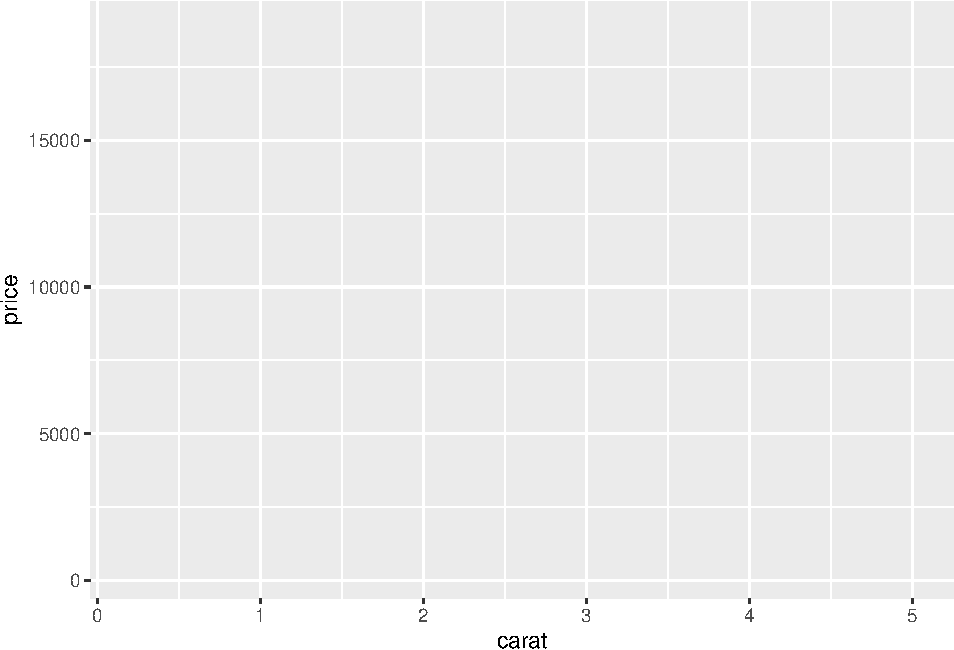
\includegraphics{Introduction-to-R,-Rstudio,-and-ggplot2_files/figure-latex/unnamed-chunk-4-1.pdf}

\begin{Shaded}
\begin{Highlighting}[]
\CommentTok{# geom_points() adds a new layer to a plot by drawing points to produce a scatter plot }
\KeywordTok{ggplot}\NormalTok{(}\DataTypeTok{data =} \NormalTok{diamonds, }\KeywordTok{aes}\NormalTok{(}\DataTypeTok{x =} \NormalTok{carat, }\DataTypeTok{y =} \NormalTok{price)) +}\StringTok{ }\KeywordTok{geom_point}\NormalTok{()}
\end{Highlighting}
\end{Shaded}

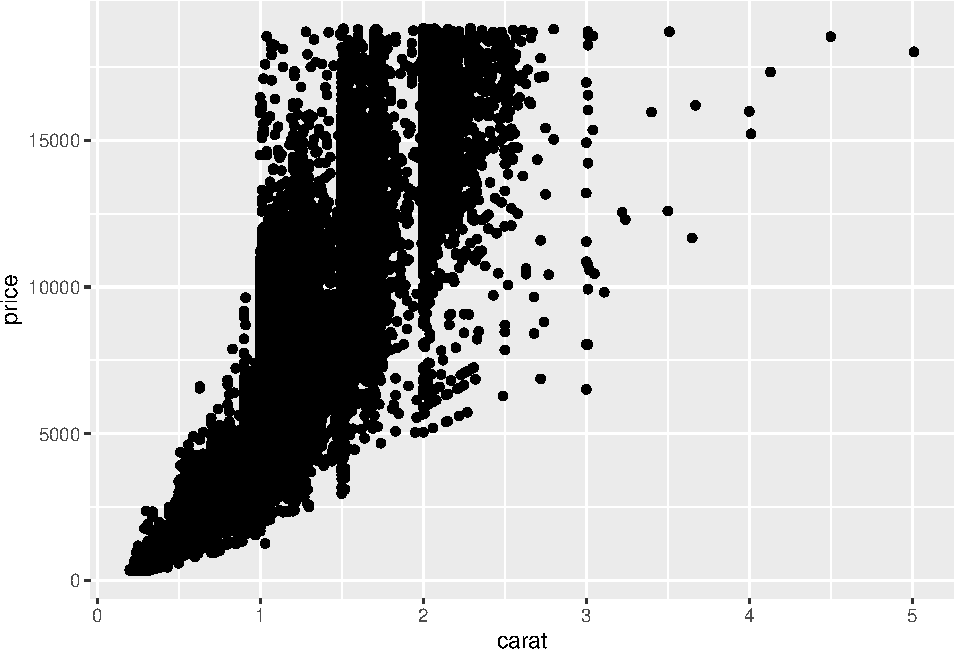
\includegraphics{Introduction-to-R,-Rstudio,-and-ggplot2_files/figure-latex/unnamed-chunk-5-1.pdf}

\begin{Shaded}
\begin{Highlighting}[]
\CommentTok{# geom_smooth() adds an additional layer to the plot by drawing a smoothed line to capture the trend in the scatterplot}
\KeywordTok{ggplot}\NormalTok{(}\DataTypeTok{data =} \NormalTok{diamonds, }\KeywordTok{aes}\NormalTok{(}\DataTypeTok{x =} \NormalTok{carat, }\DataTypeTok{y =} \NormalTok{price)) +}\StringTok{ }\KeywordTok{geom_point}\NormalTok{() +}\StringTok{ }\KeywordTok{geom_smooth}\NormalTok{()}
\end{Highlighting}
\end{Shaded}

\begin{verbatim}
## `geom_smooth()` using method = 'gam' and formula 'y ~ s(x, bs = "cs")'
\end{verbatim}

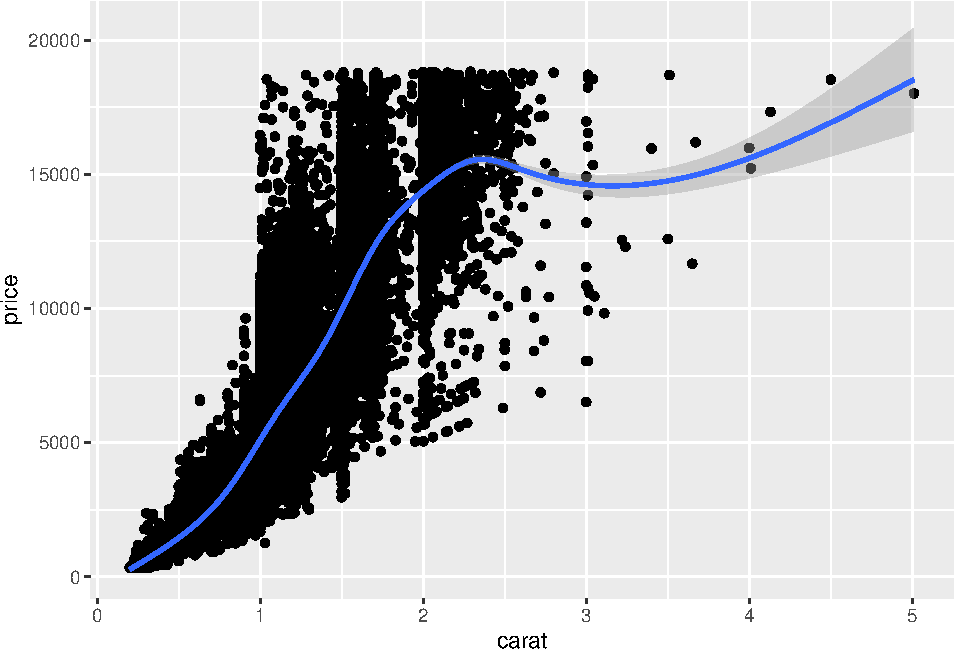
\includegraphics{Introduction-to-R,-Rstudio,-and-ggplot2_files/figure-latex/unnamed-chunk-6-1.pdf}

\section{Exercise}\label{exercise}

\begin{itemize}
\item
  typing \texttt{mtcars} in your console will display the content of the
  \texttt{mtcars} dataset. How can we display the help document for the
  \texttt{mtcars} data?
\item
  type \texttt{head(mtcars)}. What did \texttt{head()} do? Check the
  help document of \texttt{head()} (\texttt{mtcar} is a dataframe in
  base R, whereas the \texttt{diamonds} is a tibble in
  \texttt{tidyverse}).
\item
  Using the \texttt{mtcars} data, plot the scatter plot between
  \texttt{mpg} (miles per gallon: y axis) and \texttt{disp}
  (displacement: x axis) with a smoothed line.
\end{itemize}

\section{Aesthetic mappings}\label{aesthetic-mappings}

\begin{itemize}
\item
  ``A set of aesthetic mappings describe how \textbf{variables in the
  data} are mapped to \textbf{aesthetic properties} of the layer''
  \citep{ggplot2}
\item
  ``To describe the way that \textbf{variables in the data} are mapped
  to \textbf{things that we can perceive on the plot (the
  ``aesthetics'')}, we use the \texttt{aes} function. The \texttt{aes}
  function takes a list of aesthetic-variable pairs like these:
  \texttt{aes(x\ =\ weight,\ y\ =\ height,\ colour\ =\ age)}. Here we
  are mapping x-position to \texttt{weight}, y-position to
  \texttt{height} and colour to \texttt{age}. The first two arguments
  can be left without names, in which case they correspond to the x and
  y variables.'' \citep{ggplot2}
\end{itemize}

\begin{Shaded}
\begin{Highlighting}[]
\CommentTok{# color = color maps the variable 'color` in the dataset to the color aesthetics of points to encode further information in the graphic. }
\KeywordTok{ggplot}\NormalTok{(}\DataTypeTok{data =} \NormalTok{diamonds, }\KeywordTok{aes}\NormalTok{(}\DataTypeTok{x =} \NormalTok{carat, }\DataTypeTok{y =} \NormalTok{price, }\DataTypeTok{color =} \NormalTok{color)) +}\StringTok{ }\KeywordTok{geom_point}\NormalTok{()}
\end{Highlighting}
\end{Shaded}

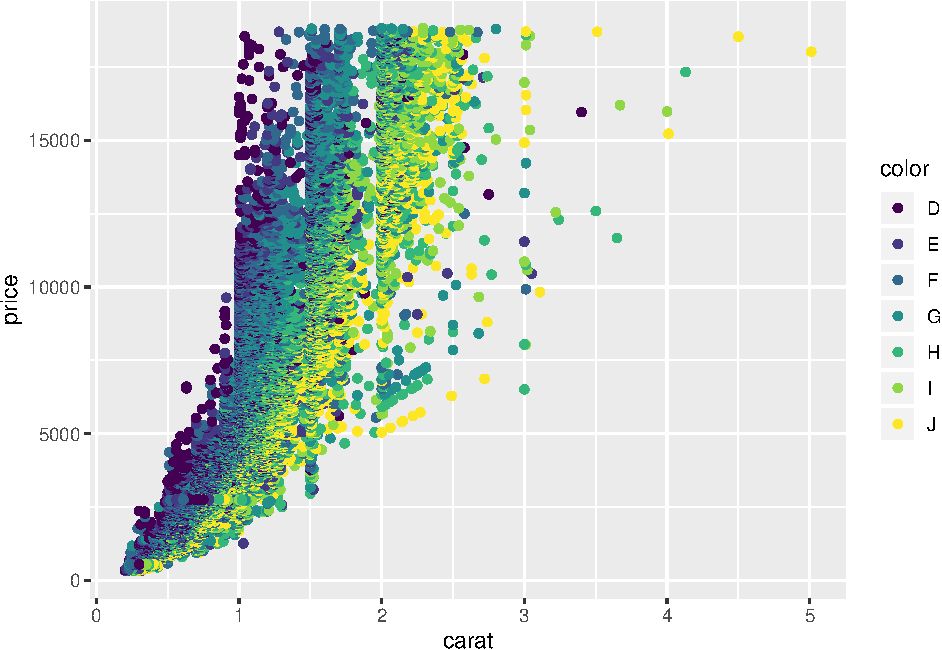
\includegraphics{Introduction-to-R,-Rstudio,-and-ggplot2_files/figure-latex/unnamed-chunk-7-1.pdf}

\begin{Shaded}
\begin{Highlighting}[]
\CommentTok{# shape = cut maps the variable 'cut` in the dataset to the shape aesthetics of points to encode further information in the graphic. }
\CommentTok{# the graphic is not so informative because points are overplotted. Sometimes, facetting may handle overplotting }
\KeywordTok{ggplot}\NormalTok{(}\DataTypeTok{data =} \NormalTok{diamonds, }\KeywordTok{aes}\NormalTok{(}\DataTypeTok{x =} \NormalTok{carat, }\DataTypeTok{y =} \NormalTok{price, }\DataTypeTok{shape =} \NormalTok{cut)) +}\StringTok{ }\KeywordTok{geom_point}\NormalTok{()}
\end{Highlighting}
\end{Shaded}

\begin{verbatim}
## Warning: Using shapes for an ordinal variable is not advised
\end{verbatim}

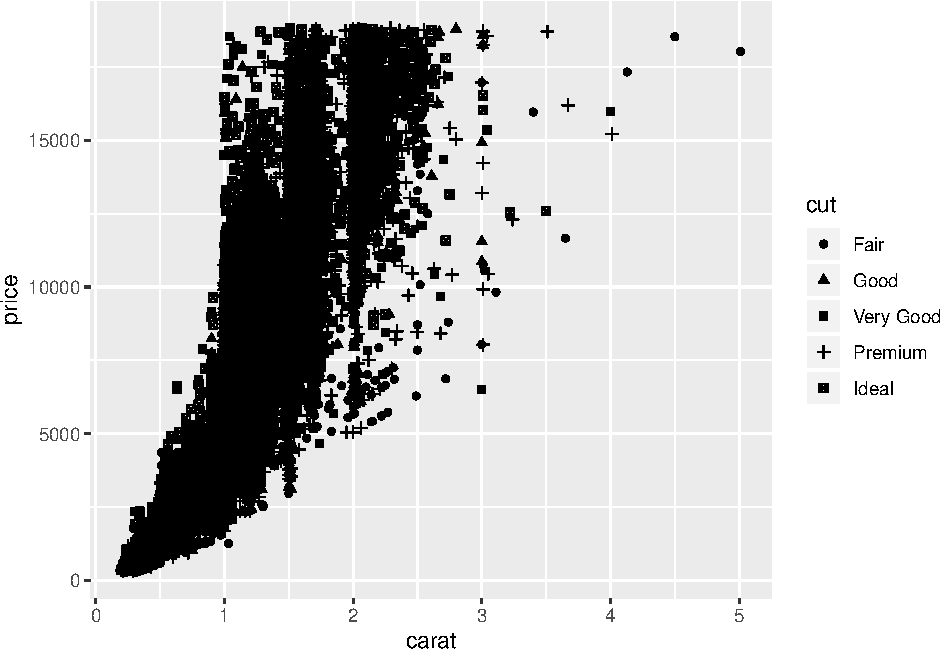
\includegraphics{Introduction-to-R,-Rstudio,-and-ggplot2_files/figure-latex/unnamed-chunk-8-1.pdf}

\begin{Shaded}
\begin{Highlighting}[]
\KeywordTok{ggplot}\NormalTok{(}\DataTypeTok{data =} \NormalTok{diamonds, }\KeywordTok{aes}\NormalTok{(}\DataTypeTok{x =} \NormalTok{carat, }\DataTypeTok{y =} \NormalTok{price)) +}\StringTok{ }\KeywordTok{geom_point}\NormalTok{(}\DataTypeTok{color =} \StringTok{"blue"}\NormalTok{)}
\end{Highlighting}
\end{Shaded}

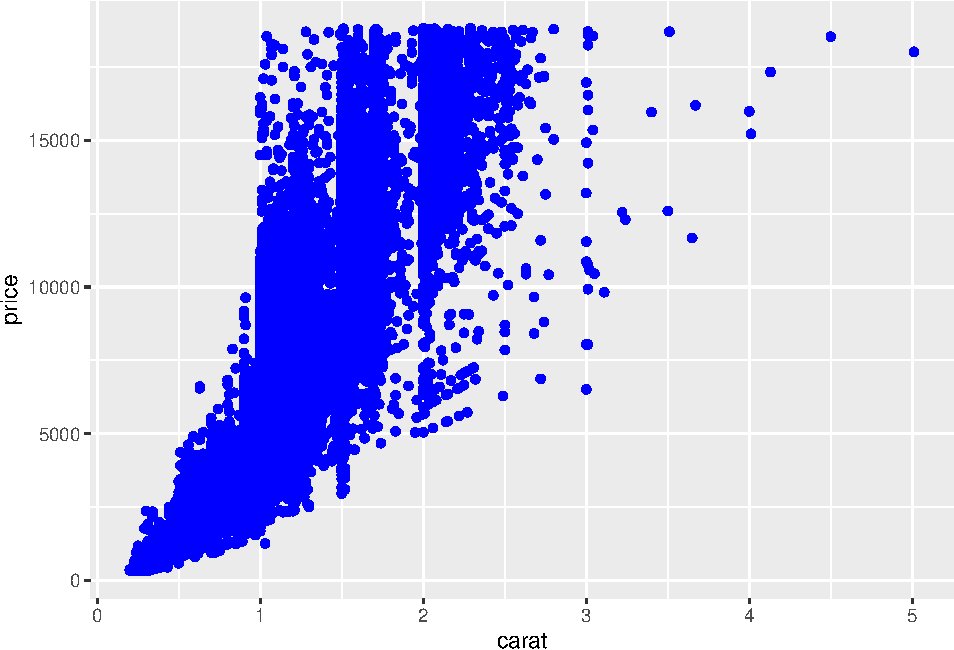
\includegraphics{Introduction-to-R,-Rstudio,-and-ggplot2_files/figure-latex/unnamed-chunk-9-1.pdf}

\section{Exercise}\label{exercise-1}

\begin{itemize}
\item
  \texttt{mpg} is similar to \texttt{mtcars} but is a built-in tibble in
  \texttt{ggplot2}. 1) Plot \texttt{hwy} (mile per gallon: y axis)
  against \texttt{displ} (engine displancement: x axis), 2) Given the
  plot from 1), map the \texttt{class} variable to color, shape, alpha,
  and size aesthetics.
\item
  Explain what happens.
\end{itemize}

\begin{Shaded}
\begin{Highlighting}[]
\KeywordTok{ggplot}\NormalTok{(}\DataTypeTok{data =} \NormalTok{mpg, }\DataTypeTok{mapping =} \KeywordTok{aes}\NormalTok{(}\DataTypeTok{x =} \NormalTok{displ, }\DataTypeTok{y =} \NormalTok{hwy, }\DataTypeTok{color=}\NormalTok{drv)) +}\StringTok{ }\KeywordTok{geom_point}\NormalTok{() +}\StringTok{ }\KeywordTok{geom_smooth}\NormalTok{(}\DataTypeTok{method=}\StringTok{"lm"}\NormalTok{)}
\end{Highlighting}
\end{Shaded}

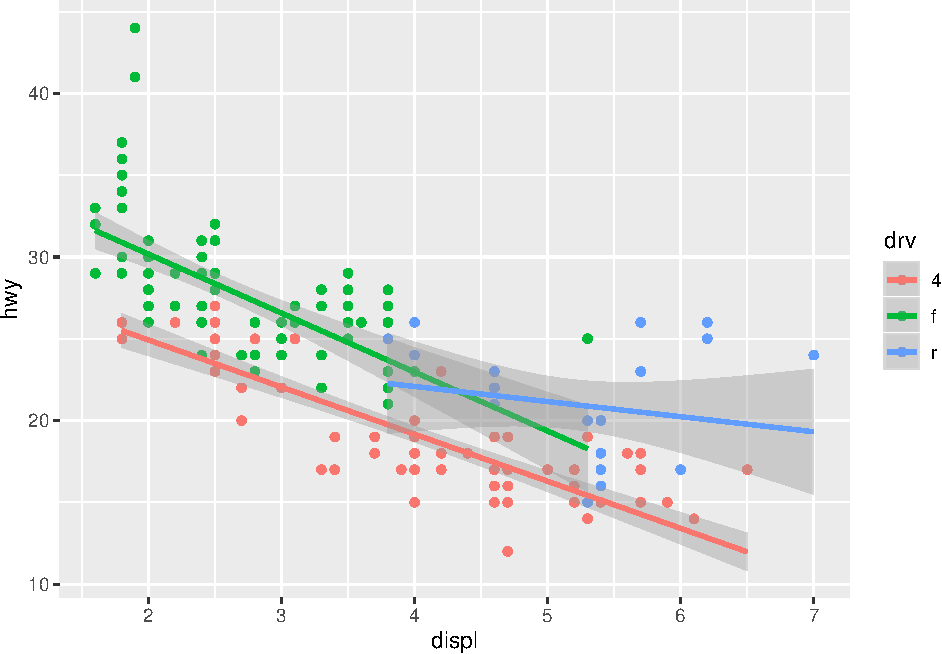
\includegraphics{Introduction-to-R,-Rstudio,-and-ggplot2_files/figure-latex/unnamed-chunk-10-1.pdf}

\begin{itemize}
\tightlist
\item
  This is what happens when mapping \texttt{hyw}, \texttt{displ}, and
  \texttt{cyl} to \texttt{x}, \texttt{y}, and \texttt{color} aesthetics.
  R creates a new dataset that contains all the data to be displayed on
  the plot.
\end{itemize}

\begin{longtable}[]{@{}lll@{}}
\toprule
x & y & color\tabularnewline
\midrule
\endhead
1.8 & 29 & 4\tabularnewline
1.8 & 29 & 4\tabularnewline
2.0 & 31 & 4\tabularnewline
2.0 & 30 & 4\tabularnewline
2.8 & 26 & 6\tabularnewline
2.8 & 26 & 6\tabularnewline
3.1 & 27 & 6\tabularnewline
1.8 & 26 & 4\tabularnewline
1.8 & 25 & 4\tabularnewline
2.0 & 28 & 4\tabularnewline
\bottomrule
\end{longtable}

\section{Scales}\label{scales}

\begin{itemize}
\item
  In the previous table, computers don't know how to display colors
  based on 4, 6, \ldots{} Computers need a a hexadecimal code for colors
  such as \texttt{FF6C91}. The mapping from the data to the final values
  that computers can use to display aesthetics is called a scale.
\item
  ``The scales map values in the data space to values in an aesthetic
  space, whether it be colour, or size, or shape. Scales draw a legend
  or axes, which provide an inverse mapping to make it possible to read
  the original data values from the graph.'' \citep{ggplot2}
\item
  \texttt{scale\_x\_continuous()} and \texttt{scale\_y\_continuous()}
  are the default scales for continuous x and y aesthetics:
  \url{https://ggplot2.tidyverse.org/reference/scale_continuous.html}.
\end{itemize}

\begin{Shaded}
\begin{Highlighting}[]
\NormalTok{p1 <-}\StringTok{ }\KeywordTok{ggplot}\NormalTok{(mpg, }\KeywordTok{aes}\NormalTok{(displ, hwy)) +}\StringTok{ }\KeywordTok{geom_point}\NormalTok{()}
\NormalTok{p1}
\end{Highlighting}
\end{Shaded}

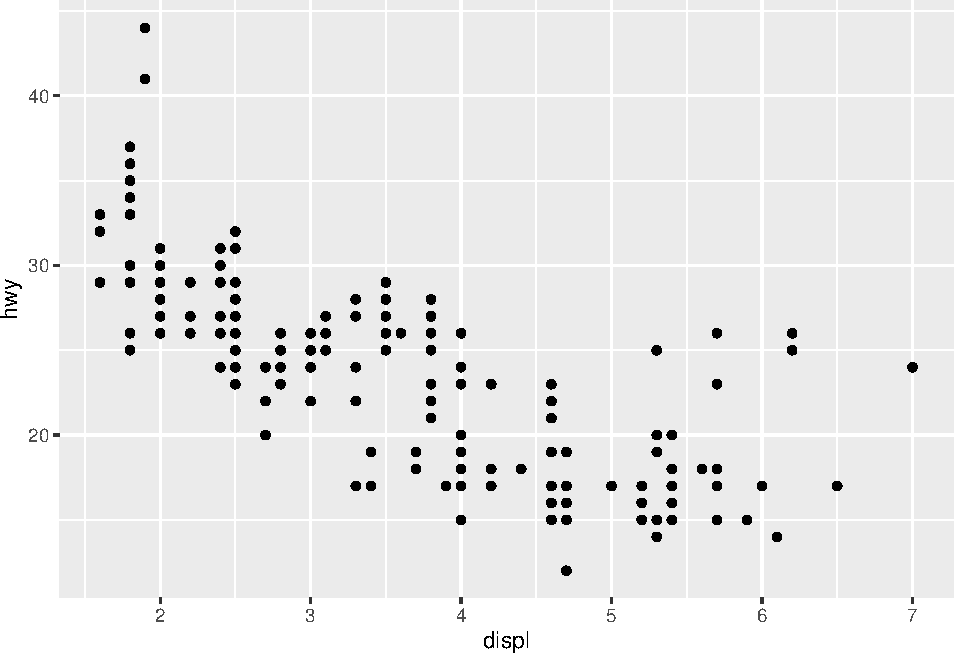
\includegraphics{Introduction-to-R,-Rstudio,-and-ggplot2_files/figure-latex/unnamed-chunk-11-1.pdf}

\begin{Shaded}
\begin{Highlighting}[]
\CommentTok{# change the axis labels}
\NormalTok{p1 +}\StringTok{ }\KeywordTok{scale_x_continuous}\NormalTok{(}\StringTok{"Engine displacement (L)"}\NormalTok{) +}
\StringTok{  }\KeywordTok{scale_y_continuous}\NormalTok{(}\StringTok{"Highway MPG"}\NormalTok{)}
\end{Highlighting}
\end{Shaded}

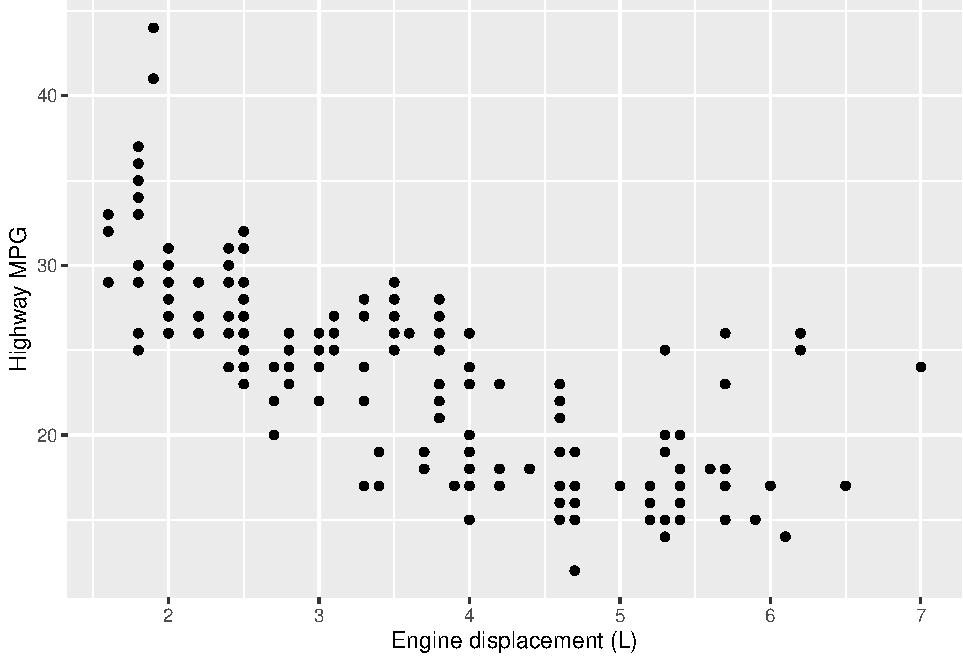
\includegraphics{Introduction-to-R,-Rstudio,-and-ggplot2_files/figure-latex/unnamed-chunk-12-1.pdf}

\begin{Shaded}
\begin{Highlighting}[]
\CommentTok{# also use the short-cut labs()}
\NormalTok{p1 +}\StringTok{ }\KeywordTok{labs}\NormalTok{(}\DataTypeTok{x =} \StringTok{"Engine displacement (L)"}\NormalTok{, }\DataTypeTok{y =} \StringTok{"Highway MPG"}\NormalTok{)}
\end{Highlighting}
\end{Shaded}

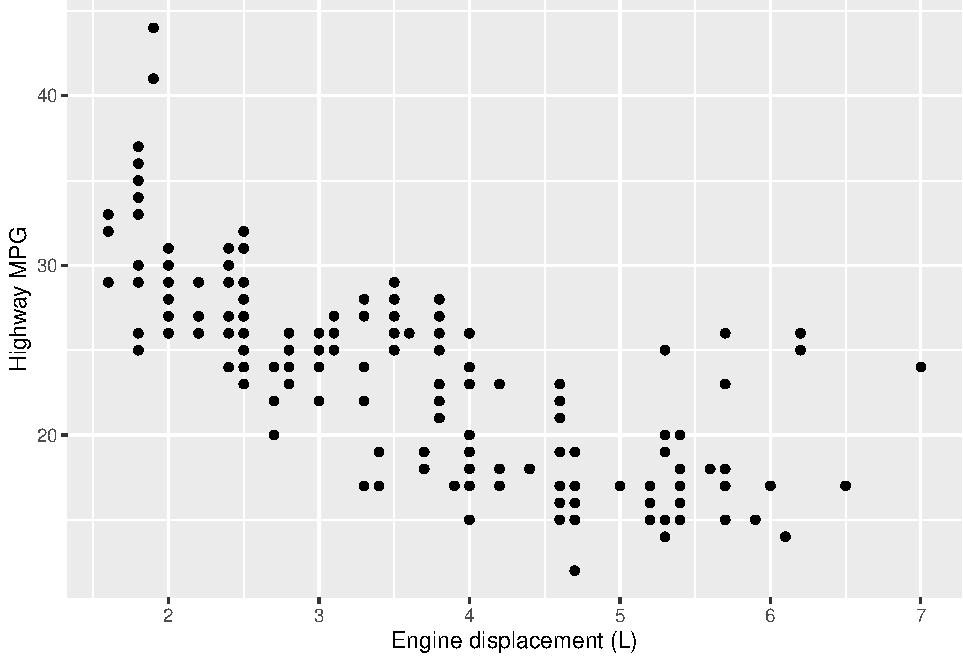
\includegraphics{Introduction-to-R,-Rstudio,-and-ggplot2_files/figure-latex/unnamed-chunk-13-1.pdf}

\begin{Shaded}
\begin{Highlighting}[]
\CommentTok{# modify the axis limits}
\NormalTok{p1 +}\StringTok{ }\KeywordTok{scale_x_continuous}\NormalTok{(}\DataTypeTok{limits =} \KeywordTok{c}\NormalTok{(}\DecValTok{2}\NormalTok{, }\DecValTok{6}\NormalTok{))}
\end{Highlighting}
\end{Shaded}

\begin{verbatim}
## Warning: Removed 27 rows containing missing values (geom_point).
\end{verbatim}

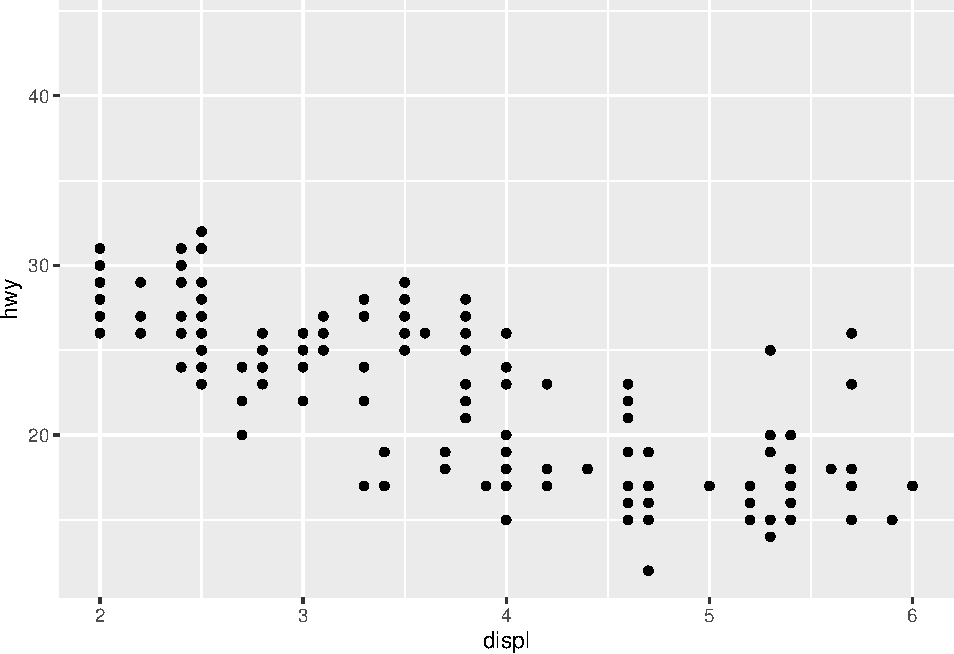
\includegraphics{Introduction-to-R,-Rstudio,-and-ggplot2_files/figure-latex/unnamed-chunk-14-1.pdf}

\begin{Shaded}
\begin{Highlighting}[]
\CommentTok{# use the short hand functions `xlim()` and `ylim()`}
\NormalTok{p1 +}\StringTok{ }\KeywordTok{xlim}\NormalTok{(}\DecValTok{2}\NormalTok{, }\DecValTok{6}\NormalTok{)}
\end{Highlighting}
\end{Shaded}

\begin{verbatim}
## Warning: Removed 27 rows containing missing values (geom_point).
\end{verbatim}

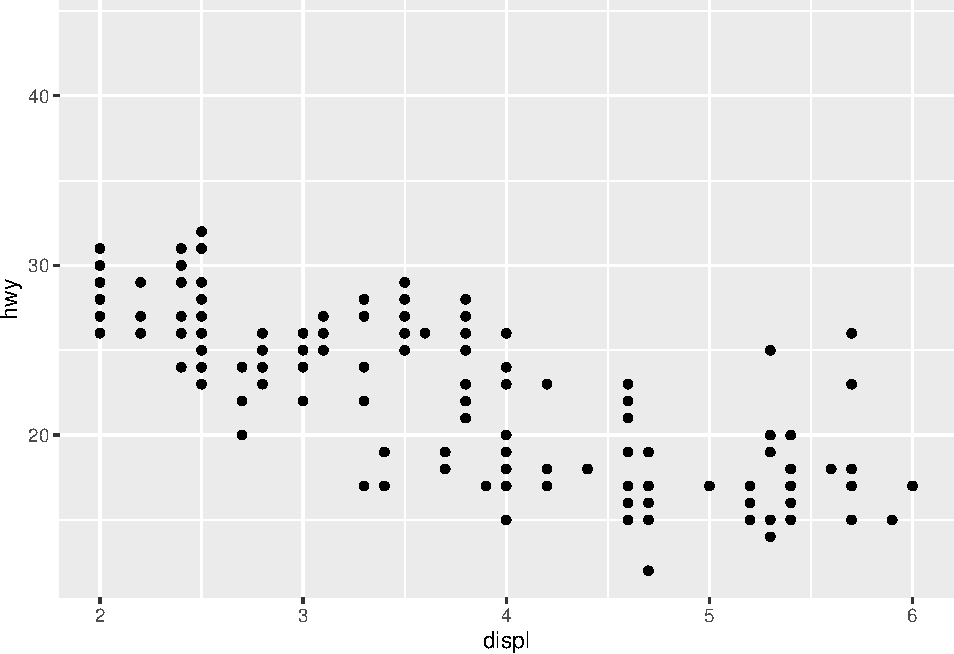
\includegraphics{Introduction-to-R,-Rstudio,-and-ggplot2_files/figure-latex/unnamed-chunk-15-1.pdf}

\begin{Shaded}
\begin{Highlighting}[]
\CommentTok{#  choose where the ticks appear}
\NormalTok{p1 +}\StringTok{ }\KeywordTok{scale_x_continuous}\NormalTok{(}\DataTypeTok{breaks =} \KeywordTok{c}\NormalTok{(}\DecValTok{2}\NormalTok{, }\DecValTok{4}\NormalTok{, }\DecValTok{6}\NormalTok{))}
\end{Highlighting}
\end{Shaded}

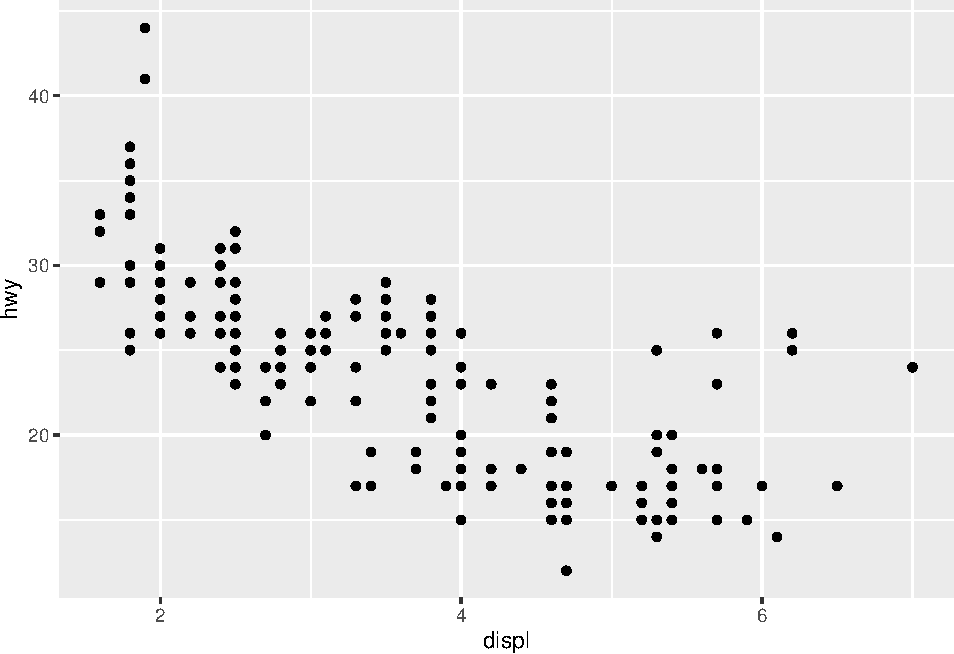
\includegraphics{Introduction-to-R,-Rstudio,-and-ggplot2_files/figure-latex/unnamed-chunk-16-1.pdf}

\begin{Shaded}
\begin{Highlighting}[]
\CommentTok{#  choose your own labels}
\NormalTok{p1 +}\StringTok{ }\KeywordTok{scale_x_continuous}\NormalTok{(}\DataTypeTok{breaks =} \KeywordTok{c}\NormalTok{(}\DecValTok{2}\NormalTok{, }\DecValTok{4}\NormalTok{, }\DecValTok{6}\NormalTok{), }\DataTypeTok{label =} \KeywordTok{c}\NormalTok{(}\StringTok{"two"}\NormalTok{, }\StringTok{"four"}\NormalTok{, }\StringTok{"six"}\NormalTok{))}
\end{Highlighting}
\end{Shaded}

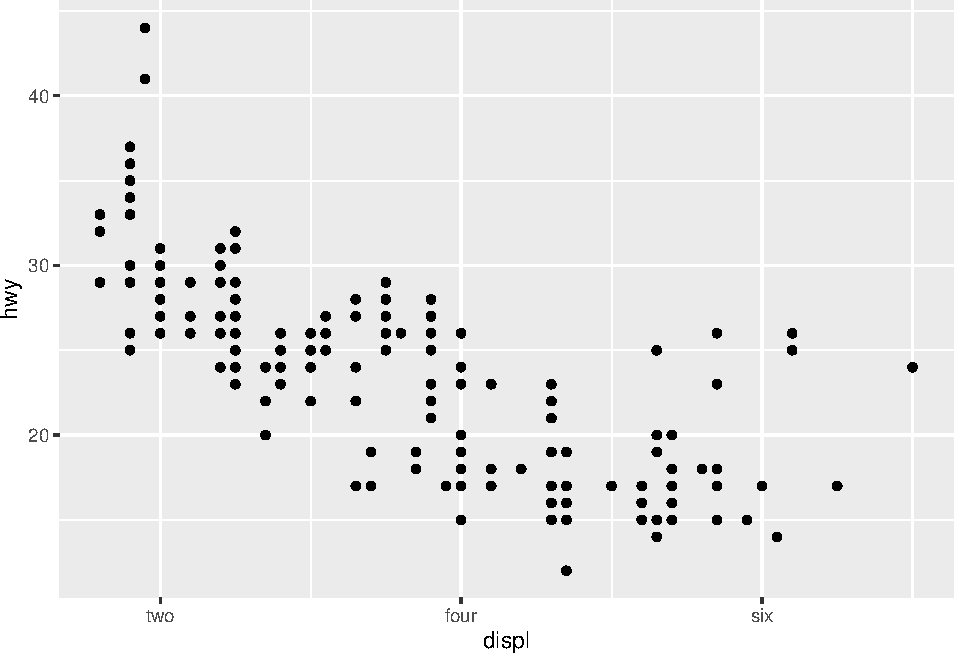
\includegraphics{Introduction-to-R,-Rstudio,-and-ggplot2_files/figure-latex/unnamed-chunk-17-1.pdf}

\begin{Shaded}
\begin{Highlighting}[]
\KeywordTok{ggplot}\NormalTok{(}\DataTypeTok{data =} \NormalTok{mpg, }\DataTypeTok{mapping =} \KeywordTok{aes}\NormalTok{(}\DataTypeTok{x =} \NormalTok{displ, }\DataTypeTok{y =} \NormalTok{hwy, }\DataTypeTok{color=}\NormalTok{drv)) +}\StringTok{ }\KeywordTok{geom_point}\NormalTok{() +}\StringTok{ }\KeywordTok{geom_smooth}\NormalTok{(}\DataTypeTok{method=}\StringTok{"lm"}\NormalTok{) +}\StringTok{ }\KeywordTok{labs}\NormalTok{(}\DataTypeTok{title =}\StringTok{"MPG vs Engine size"}\NormalTok{, }\DataTypeTok{x =} \StringTok{"Engine size"}\NormalTok{, }\DataTypeTok{y =} \StringTok{"MPG"}\NormalTok{)}
\end{Highlighting}
\end{Shaded}

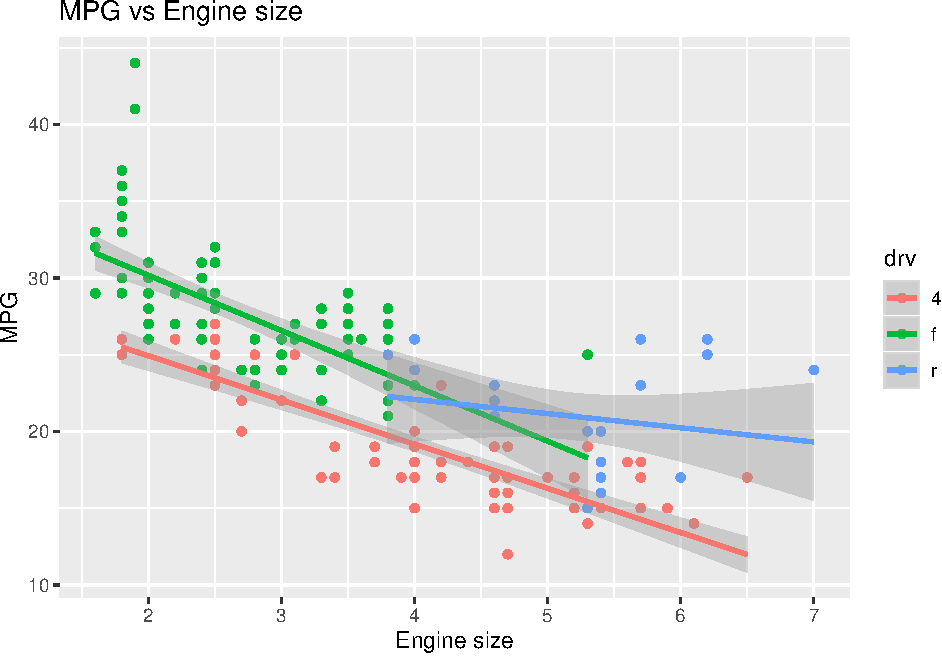
\includegraphics{Introduction-to-R,-Rstudio,-and-ggplot2_files/figure-latex/unnamed-chunk-18-1.pdf}

\begin{Shaded}
\begin{Highlighting}[]
\CommentTok{# Create your own discrete scale}
\KeywordTok{ggplot}\NormalTok{(}\DataTypeTok{data =} \NormalTok{mpg, }\DataTypeTok{mapping =} \KeywordTok{aes}\NormalTok{(}\DataTypeTok{x =} \NormalTok{displ, }\DataTypeTok{y =} \NormalTok{hwy, }\DataTypeTok{color=}\NormalTok{drv)) +}\StringTok{ }\KeywordTok{geom_point}\NormalTok{() +}\StringTok{ }\KeywordTok{geom_smooth}\NormalTok{(}\DataTypeTok{method=}\StringTok{"lm"}\NormalTok{) +}\StringTok{ }\KeywordTok{labs}\NormalTok{(}\DataTypeTok{title =}\StringTok{"MPG vs Engine size"}\NormalTok{, }\DataTypeTok{x =} \StringTok{"Engine size"}\NormalTok{, }\DataTypeTok{y =} \StringTok{"MPG"}\NormalTok{) +}\StringTok{ }\KeywordTok{scale_colour_manual}\NormalTok{(}\DataTypeTok{name =} \StringTok{"Drive"}\NormalTok{, }\DataTypeTok{values =} \KeywordTok{c}\NormalTok{(}\StringTok{"lightpink"}\NormalTok{, }\StringTok{"darkseagreen"}\NormalTok{, }\StringTok{"lightblue"}\NormalTok{))}
\end{Highlighting}
\end{Shaded}

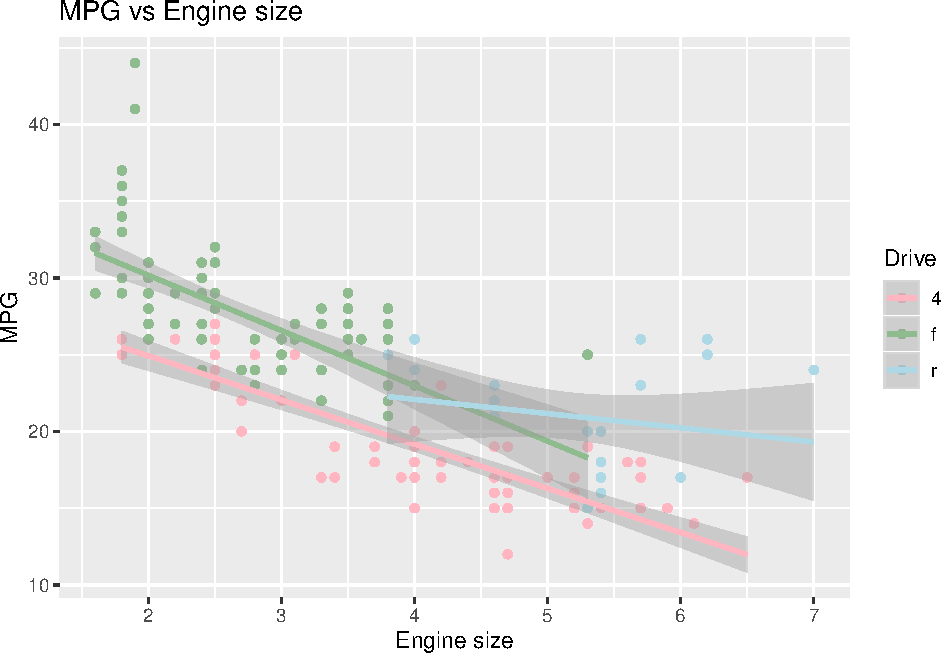
\includegraphics{Introduction-to-R,-Rstudio,-and-ggplot2_files/figure-latex/unnamed-chunk-19-1.pdf}

\begin{Shaded}
\begin{Highlighting}[]
\KeywordTok{ggplot}\NormalTok{(}\DataTypeTok{data =} \NormalTok{mpg, }\DataTypeTok{mapping =} \KeywordTok{aes}\NormalTok{(}\DataTypeTok{x =} \NormalTok{displ, }\DataTypeTok{y =} \NormalTok{hwy, }\DataTypeTok{color=}\NormalTok{cty)) +}\StringTok{ }\KeywordTok{geom_point}\NormalTok{() }
\end{Highlighting}
\end{Shaded}

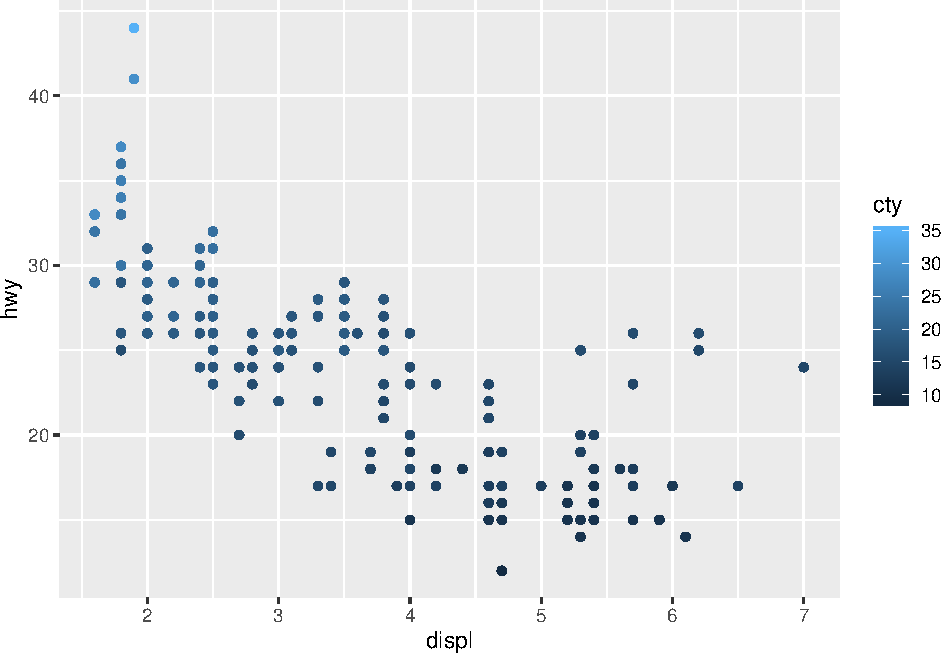
\includegraphics{Introduction-to-R,-Rstudio,-and-ggplot2_files/figure-latex/unnamed-chunk-20-1.pdf}

\begin{Shaded}
\begin{Highlighting}[]
\KeywordTok{ggplot}\NormalTok{(}\DataTypeTok{data =} \NormalTok{mpg, }\DataTypeTok{mapping =} \KeywordTok{aes}\NormalTok{(}\DataTypeTok{x =} \NormalTok{displ, }\DataTypeTok{y =} \NormalTok{hwy, }\DataTypeTok{color=}\NormalTok{cty)) +}\StringTok{ }\KeywordTok{geom_point}\NormalTok{() +}\StringTok{ }\KeywordTok{scale_colour_gradient}\NormalTok{(}\DataTypeTok{name =} \StringTok{"City MPG"}\NormalTok{, }\DataTypeTok{low =} \StringTok{"red"}\NormalTok{, }\DataTypeTok{high =} \StringTok{"blue"}\NormalTok{)}
\end{Highlighting}
\end{Shaded}

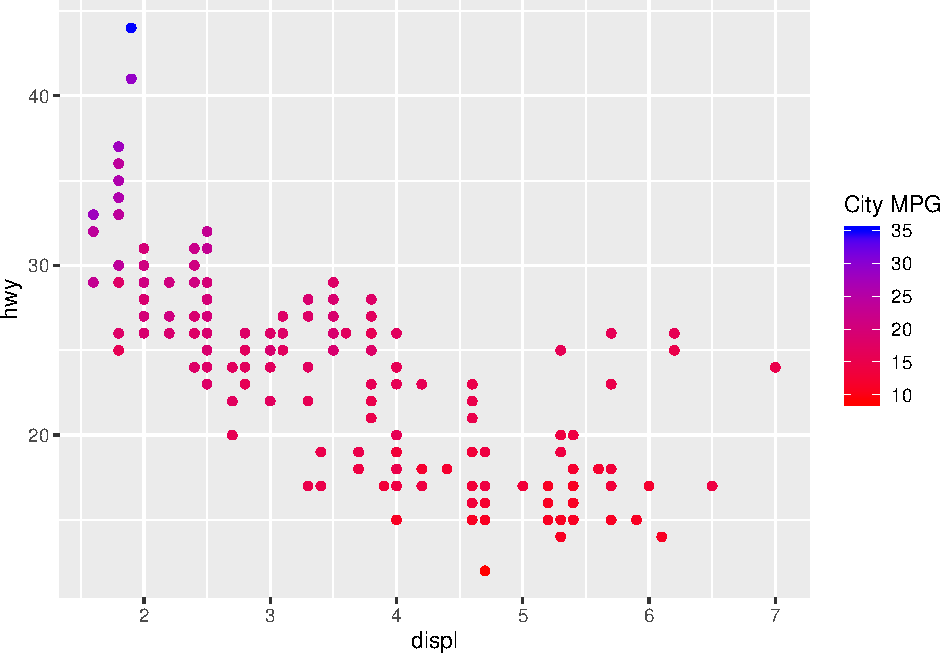
\includegraphics{Introduction-to-R,-Rstudio,-and-ggplot2_files/figure-latex/unnamed-chunk-21-1.pdf}

\begin{itemize}
\item
  For more details about scales, see
  \url{https://ggplot2.tidyverse.org/reference/}.
\item
  Colors in R: \url{http://www.sthda.com/english/wiki/colors-in-r}
\end{itemize}

\section{\texorpdfstring{Statistical transformations (\textbf{stats} for
short)}{Statistical transformations (stats for short)}}\label{statistical-transformations-stats-for-short}

\begin{Shaded}
\begin{Highlighting}[]
\CommentTok{# historam shows the distribution of a single variable. }
\CommentTok{# where does count come from? }
\KeywordTok{ggplot}\NormalTok{(}\DataTypeTok{data =} \NormalTok{diamonds, }\KeywordTok{aes}\NormalTok{(}\DataTypeTok{x =} \NormalTok{carat)) +}\StringTok{ }\KeywordTok{geom_histogram}\NormalTok{()}
\end{Highlighting}
\end{Shaded}

\begin{verbatim}
## `stat_bin()` using `bins = 30`. Pick better value with `binwidth`.
\end{verbatim}

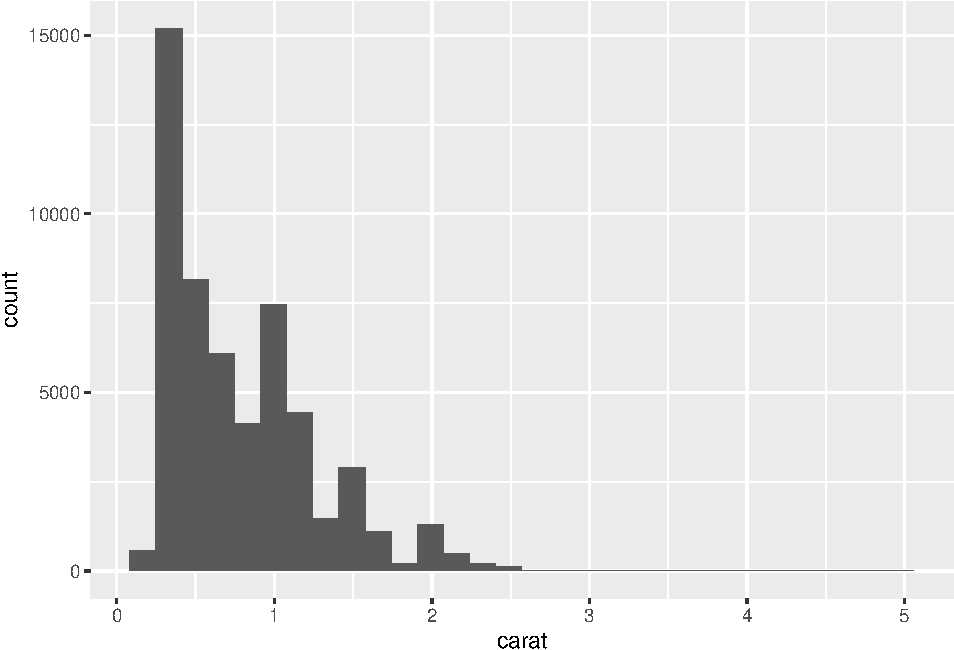
\includegraphics{Introduction-to-R,-Rstudio,-and-ggplot2_files/figure-latex/unnamed-chunk-22-1.pdf}

\begin{itemize}
\item
  ``Statistical transformations, \textbf{stats} for short, summarise
  data in many useful ways. For example, binning and counting
  observations to create a histogram, or summarising a 2d relationship
  with a linear model. Stats are optional, but very useful.''
  \citep{ggplot2}
\item
  How \texttt{geom\_histogram()} works?

  \begin{itemize}
  \tightlist
  \item
    ``A stat takes a dataset as input and returns a dataset as output,
    and so a stat can add new variables to the original dataset. It is
    possible to map aesthetics to these new variables. For example,
    \texttt{stat\_bin}, the statistic used to make histograms, produces
    the following variables:

    \begin{itemize}
    \tightlist
    \item
      \texttt{count}, the number of observations in each bin
    \item
      \texttt{density}, the density of observations in each bin
      (percentage of total / bar width)
    \item
      \texttt{x}, the centre of the bin" \citep{ggplot2}
    \end{itemize}
  \item
    ``These generated variables can be used instead of the variables
    present in the original dataset. For example, the default histogram
    geom assigns the height of the bars to the number of observations
    (\texttt{count}), but if you'd prefer a more traditional histogram,
    you can use the density (\texttt{density}). The following example
    shows a density histogram of carat from the diamonds dataset.''
    \citep{ggplot2}
  \end{itemize}
\end{itemize}

\begin{Shaded}
\begin{Highlighting}[]
\CommentTok{# The names of generated variables must be surrounded with ..}
 \KeywordTok{ggplot}\NormalTok{(diamonds, }\KeywordTok{aes}\NormalTok{(carat)) +}\StringTok{ }\KeywordTok{geom_histogram}\NormalTok{(}\KeywordTok{aes}\NormalTok{(}\DataTypeTok{y =} \NormalTok{..density..), }\DataTypeTok{binwidth =} \FloatTok{0.1}\NormalTok{)}
\end{Highlighting}
\end{Shaded}

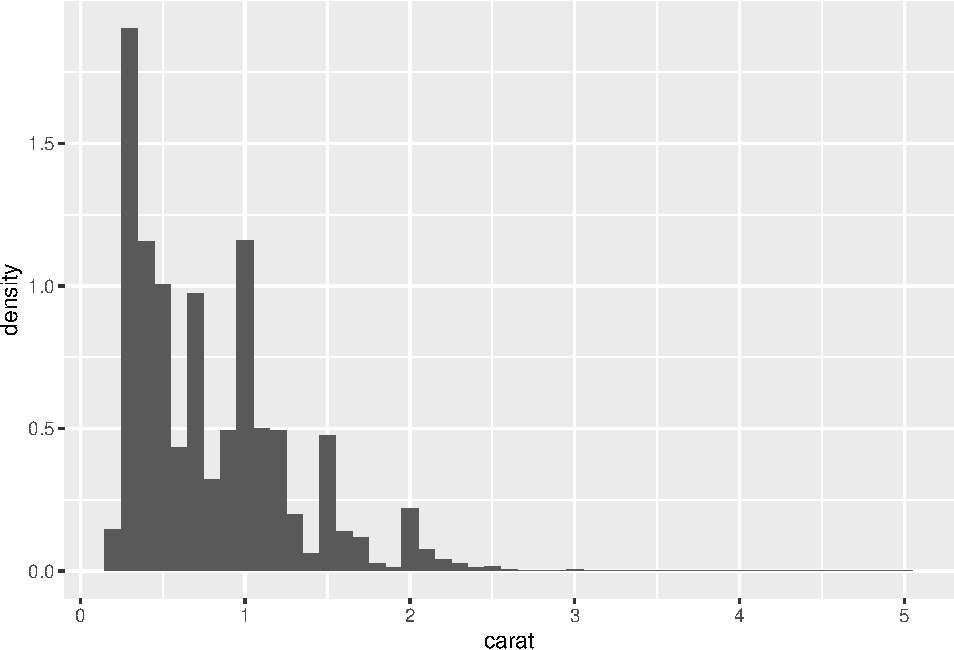
\includegraphics{Introduction-to-R,-Rstudio,-and-ggplot2_files/figure-latex/unnamed-chunk-23-1.pdf}

\begin{itemize}
\item
  Every \textbf{geom} has a default \textbf{stats}.
\item
  Position adjustments

  \begin{itemize}
  \tightlist
  \item
    Position adjustments determine how to arrange \textbf{geoms} that
    would otherwise occupy the same space.
  \end{itemize}
\end{itemize}

\begin{Shaded}
\begin{Highlighting}[]
\CommentTok{# The discrete analogue of histogram is the bar plot}
\NormalTok{s <-}\StringTok{ }\KeywordTok{ggplot}\NormalTok{(mpg, }\KeywordTok{aes}\NormalTok{(fl, }\DataTypeTok{fill =} \NormalTok{drv))}
\end{Highlighting}
\end{Shaded}

\begin{Shaded}
\begin{Highlighting}[]
\NormalTok{s +}\StringTok{ }\KeywordTok{geom_bar}\NormalTok{()}
\end{Highlighting}
\end{Shaded}

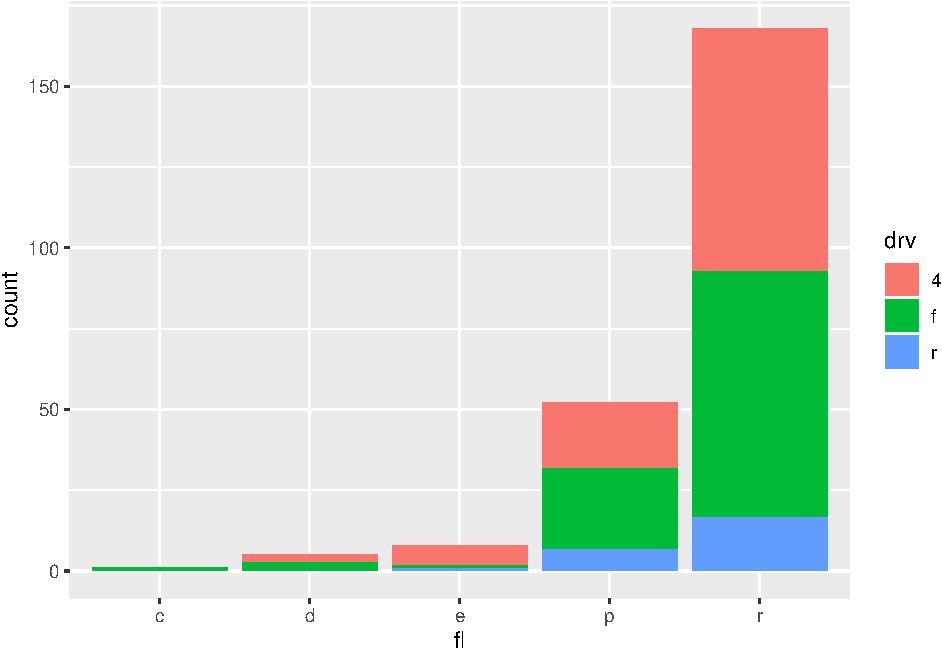
\includegraphics{Introduction-to-R,-Rstudio,-and-ggplot2_files/figure-latex/unnamed-chunk-25-1.pdf}

\begin{Shaded}
\begin{Highlighting}[]
\CommentTok{# Stack elements on top of one another}
\NormalTok{s +}\StringTok{ }\KeywordTok{geom_bar}\NormalTok{(}\DataTypeTok{position =} \StringTok{"stack"}\NormalTok{)}
\end{Highlighting}
\end{Shaded}

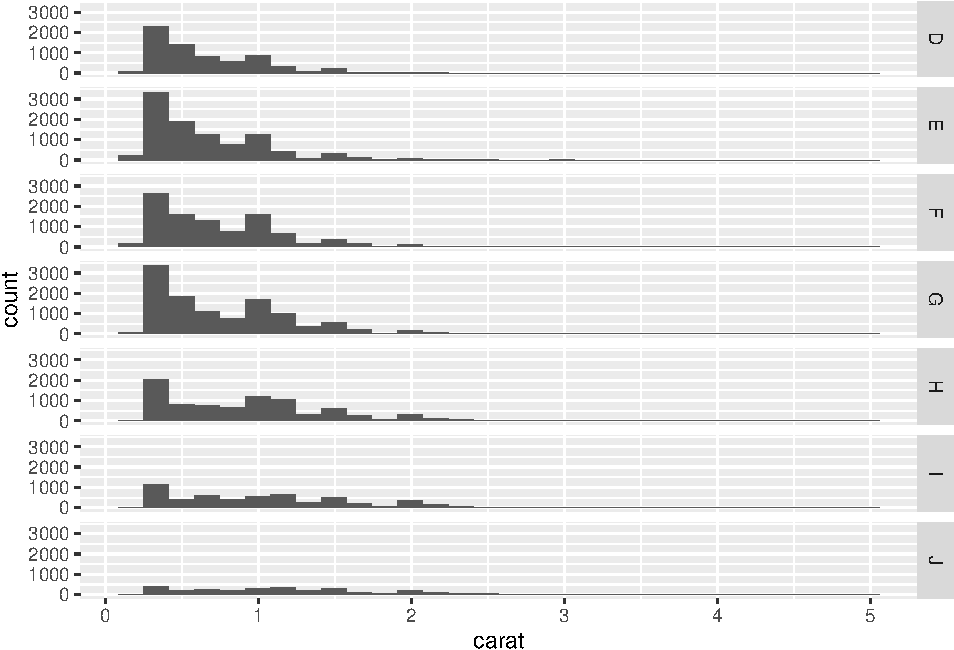
\includegraphics{Introduction-to-R,-Rstudio,-and-ggplot2_files/figure-latex/unnamed-chunk-26-1.pdf}

\begin{Shaded}
\begin{Highlighting}[]
\CommentTok{# Arrange elements side by side}
\NormalTok{s +}\StringTok{ }\KeywordTok{geom_bar}\NormalTok{(}\DataTypeTok{position =} \StringTok{"dodge"}\NormalTok{)}
\end{Highlighting}
\end{Shaded}

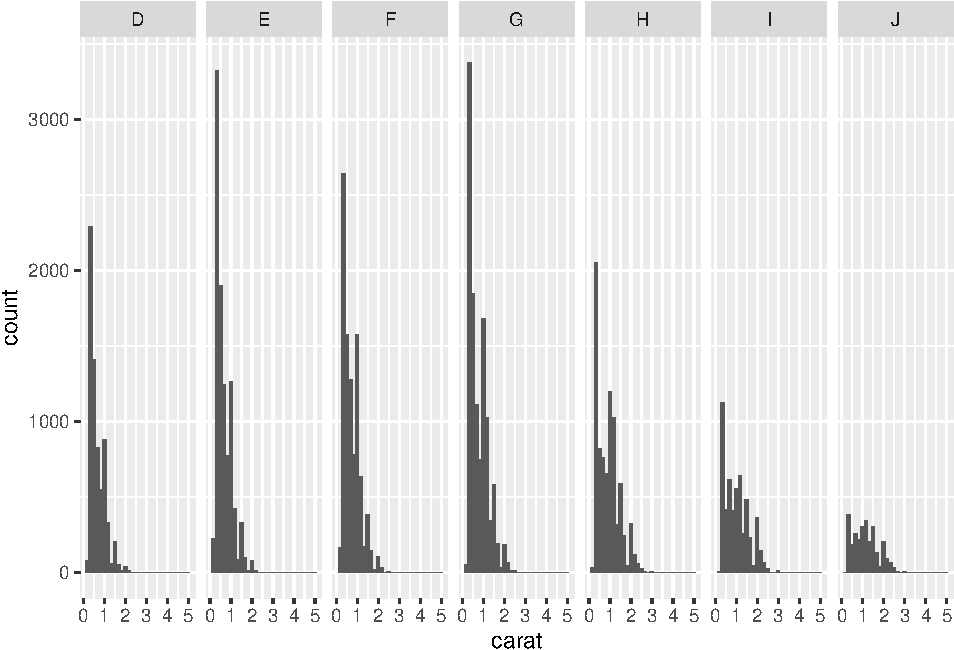
\includegraphics{Introduction-to-R,-Rstudio,-and-ggplot2_files/figure-latex/unnamed-chunk-27-1.pdf}

\begin{Shaded}
\begin{Highlighting}[]
\CommentTok{# Stack elements on top of one another,normalize height}
\NormalTok{s +}\StringTok{ }\KeywordTok{geom_bar}\NormalTok{(}\DataTypeTok{position =} \StringTok{"fill"}\NormalTok{)}
\end{Highlighting}
\end{Shaded}

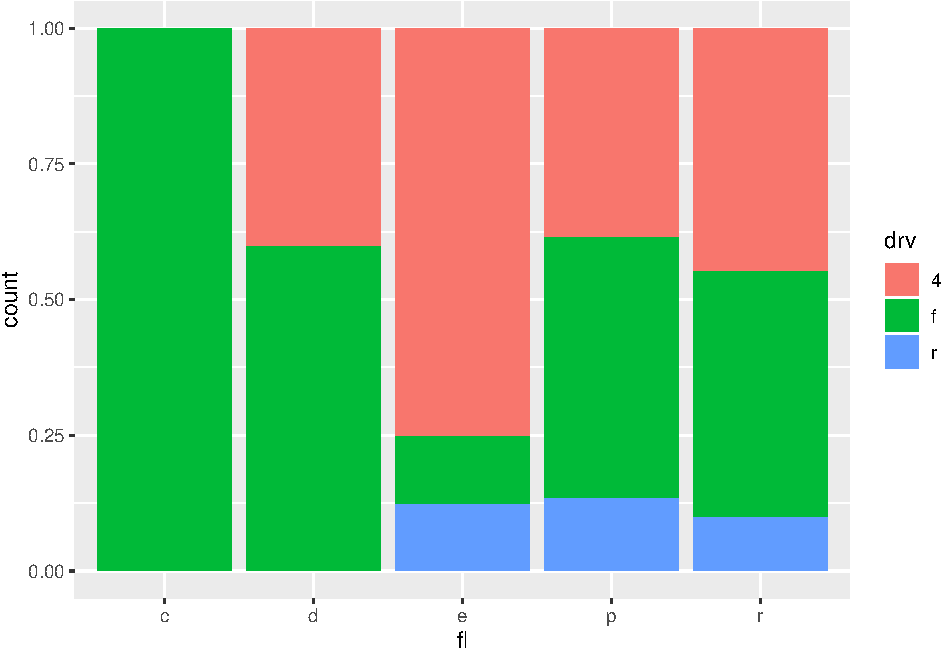
\includegraphics{Introduction-to-R,-Rstudio,-and-ggplot2_files/figure-latex/unnamed-chunk-28-1.pdf}

\section{A faceting}\label{a-faceting}

\begin{itemize}
\item
  ``A faceting specification describes how to break up the data into
  \textbf{subsets} and how to display those subsets as \textbf{small
  multiples}. This is also known as \textbf{conditioning} or
  latticing/trellising.'' \citep{ggplot2}
\item
  ``There are two types of faceting provided by ggplot2:
  \texttt{facet\_grid} and \texttt{facet\_wrap}. Facet grid produces a
  2d grid of panels defined by variables which form the rows and
  columns, while facet wrap produces a 1d ribbon of panels that is
  wrapped into 2d'' \citep{ggplot2}
\end{itemize}

\begin{Shaded}
\begin{Highlighting}[]
\CommentTok{# facet into rows}
\KeywordTok{ggplot}\NormalTok{(}\DataTypeTok{data =} \NormalTok{diamonds, }\KeywordTok{aes}\NormalTok{(}\DataTypeTok{x =} \NormalTok{carat)) +}\StringTok{ }\KeywordTok{geom_histogram}\NormalTok{() +}\StringTok{ }\KeywordTok{facet_grid}\NormalTok{(color ~}\StringTok{ }\NormalTok{.)}
\end{Highlighting}
\end{Shaded}

\begin{verbatim}
## `stat_bin()` using `bins = 30`. Pick better value with `binwidth`.
\end{verbatim}

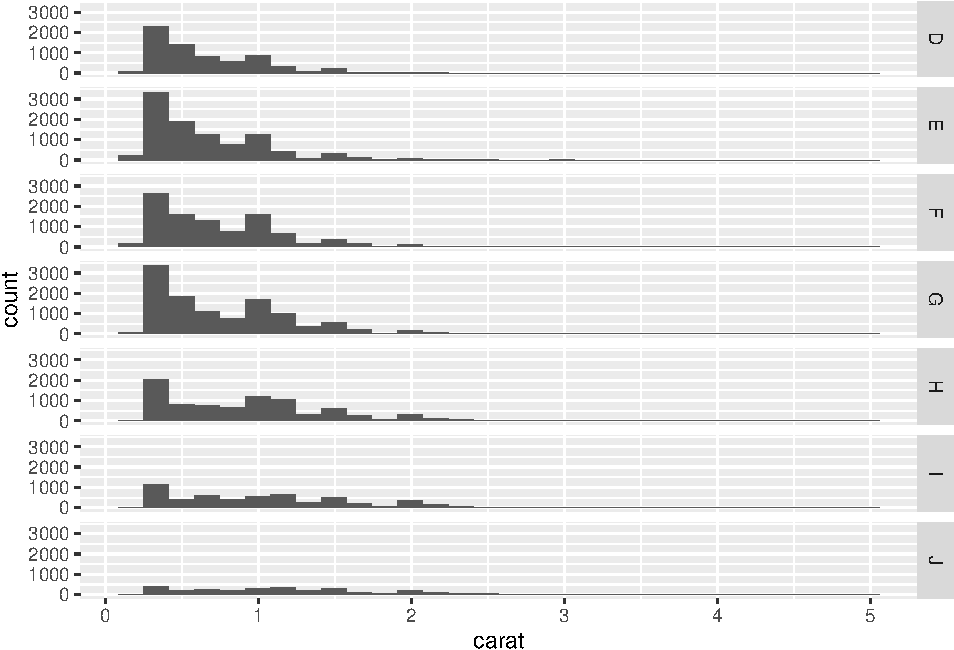
\includegraphics{Introduction-to-R,-Rstudio,-and-ggplot2_files/figure-latex/unnamed-chunk-29-1.pdf}

\begin{Shaded}
\begin{Highlighting}[]
\CommentTok{# facet into columns}
\KeywordTok{ggplot}\NormalTok{(}\DataTypeTok{data =} \NormalTok{diamonds, }\KeywordTok{aes}\NormalTok{(}\DataTypeTok{x =} \NormalTok{carat)) +}\StringTok{ }\KeywordTok{geom_histogram}\NormalTok{() +}\StringTok{ }\KeywordTok{facet_grid}\NormalTok{(. ~}\StringTok{ }\NormalTok{color)}
\end{Highlighting}
\end{Shaded}

\begin{verbatim}
## `stat_bin()` using `bins = 30`. Pick better value with `binwidth`.
\end{verbatim}

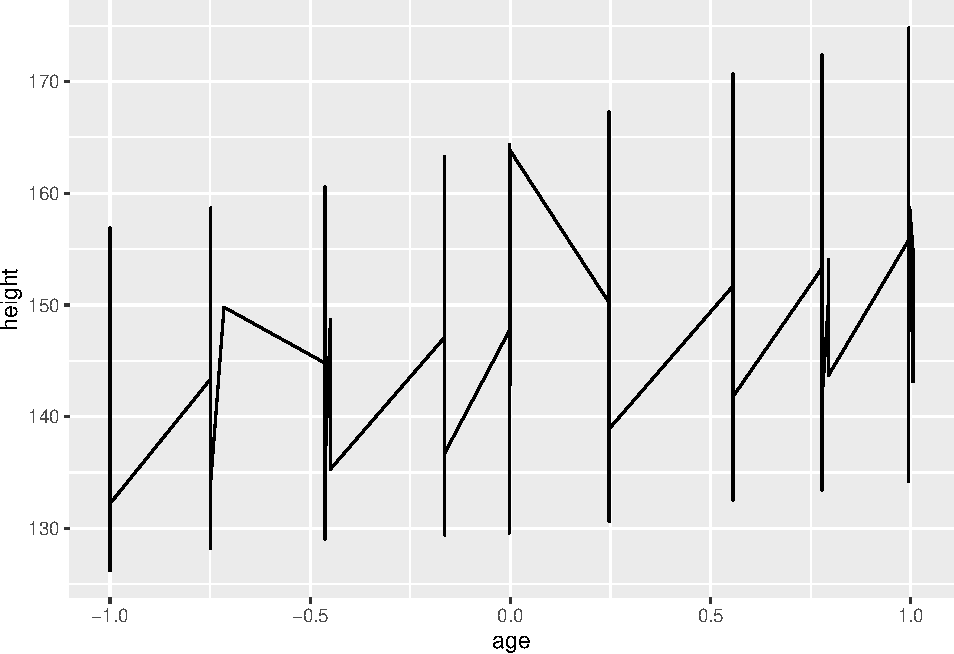
\includegraphics{Introduction-to-R,-Rstudio,-and-ggplot2_files/figure-latex/unnamed-chunk-30-1.pdf}

\section{Exercise}\label{exercise-2}

\begin{itemize}
\item
  Using \texttt{mpg} data, plot \texttt{hwy} (y) vs \texttt{cty} (x).
\item
  facet into rows using \texttt{cyl}.
\item
  facet into columns using \texttt{cyl}.
\item
  facet into rows using \texttt{cyl} and columns using \texttt{year}
\end{itemize}

\section{Grouping}\label{grouping}

\begin{itemize}
\item
  ``In many situations, you want to \textbf{separate your data into
  groups}, but render them in the same way. When looking at the data in
  aggregate you want to be able to distinguish individual subjects, but
  not identify them. This is common in \textbf{longitudinal studies}
  with many subjects, where the plots are often descriptively called
  spaghetti plots.'' \citep{ggplot2}
\item
  \texttt{Oxboys} is a dataset in the \texttt{nlme} package.
  \texttt{Oxboys} includes the height of a selection of boys from
  Oxford, England versus a standardized age.
\end{itemize}

\begin{Shaded}
\begin{Highlighting}[]
\KeywordTok{library}\NormalTok{(nlme)}
\end{Highlighting}
\end{Shaded}

\begin{Shaded}
\begin{Highlighting}[]
\CommentTok{# age = a numeric vector giving the standardized age }
\KeywordTok{head}\NormalTok{(Oxboys)}
\end{Highlighting}
\end{Shaded}

\begin{verbatim}
## Grouped Data: height ~ age | Subject
##   Subject     age height Occasion
## 1       1 -1.0000  140.5        1
## 2       1 -0.7479  143.4        2
## 3       1 -0.4630  144.8        3
## 4       1 -0.1643  147.1        4
## 5       1 -0.0027  147.7        5
## 6       1  0.2466  150.2        6
\end{verbatim}

\begin{Shaded}
\begin{Highlighting}[]
\KeywordTok{ggplot}\NormalTok{(Oxboys, }\KeywordTok{aes}\NormalTok{(age, height)) +}\StringTok{ }\KeywordTok{geom_line}\NormalTok{()}
\end{Highlighting}
\end{Shaded}

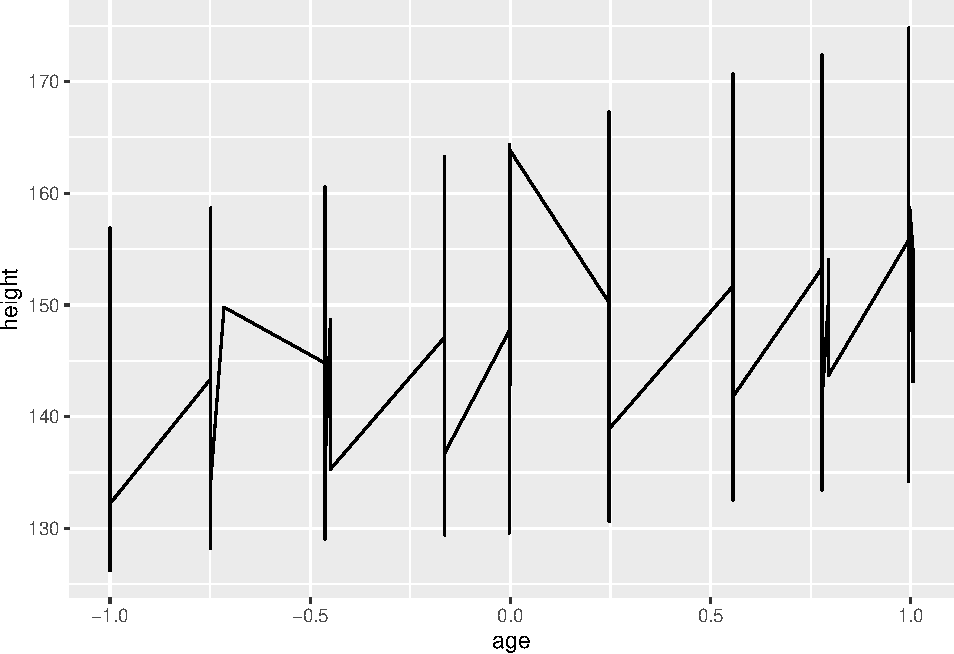
\includegraphics{Introduction-to-R,-Rstudio,-and-ggplot2_files/figure-latex/unnamed-chunk-33-1.pdf}

\begin{Shaded}
\begin{Highlighting}[]
\KeywordTok{ggplot}\NormalTok{(Oxboys, }\KeywordTok{aes}\NormalTok{(age, height, }\DataTypeTok{group =} \NormalTok{Subject)) +}\StringTok{ }\KeywordTok{geom_line}\NormalTok{()}
\end{Highlighting}
\end{Shaded}

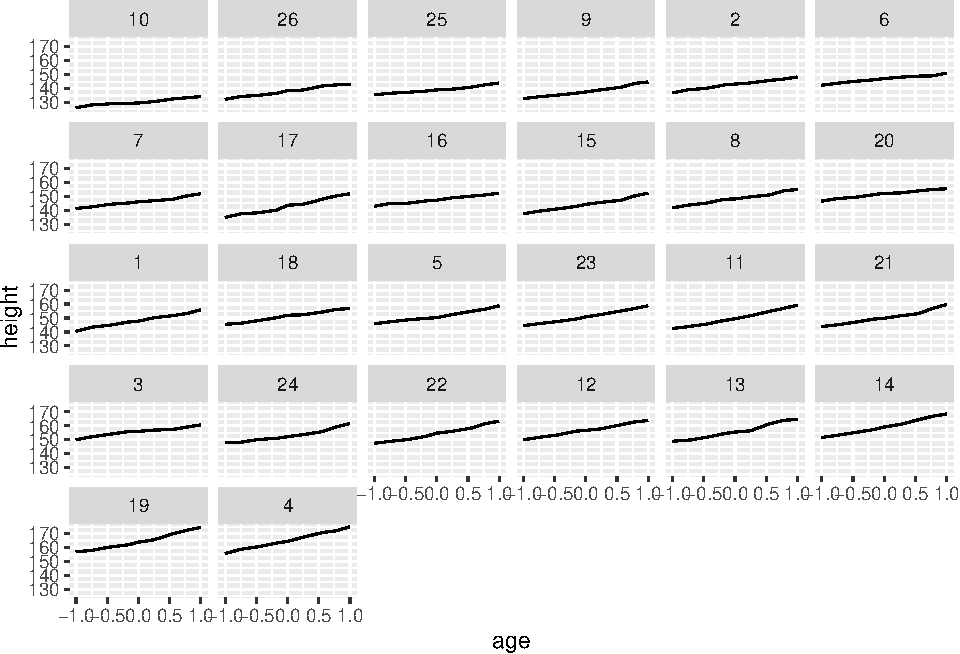
\includegraphics{Introduction-to-R,-Rstudio,-and-ggplot2_files/figure-latex/unnamed-chunk-34-1.pdf}

\begin{Shaded}
\begin{Highlighting}[]
\CommentTok{# In many cases, this is not what we want}
\KeywordTok{ggplot}\NormalTok{(Oxboys, }\KeywordTok{aes}\NormalTok{(age, height, }\DataTypeTok{group =} \NormalTok{Subject)) +}\StringTok{ }\KeywordTok{geom_line}\NormalTok{() +}\StringTok{ }\KeywordTok{geom_smooth}\NormalTok{()}
\end{Highlighting}
\end{Shaded}

\begin{verbatim}
## `geom_smooth()` using method = 'loess' and formula 'y ~ x'
\end{verbatim}

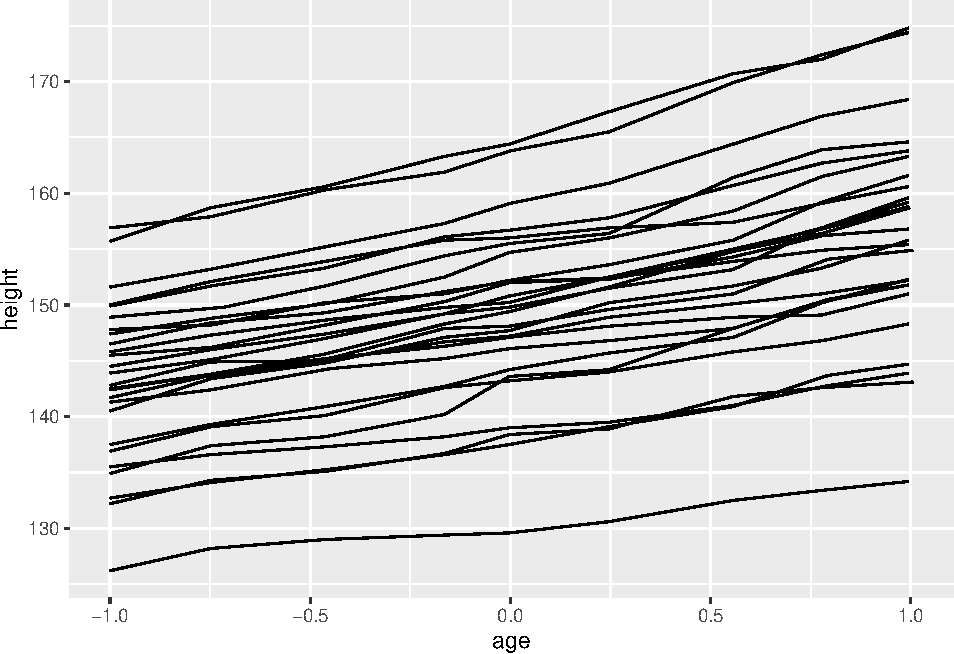
\includegraphics{Introduction-to-R,-Rstudio,-and-ggplot2_files/figure-latex/unnamed-chunk-35-1.pdf}

\begin{Shaded}
\begin{Highlighting}[]
\CommentTok{# group = 1 override the default grouping }
\KeywordTok{ggplot}\NormalTok{(Oxboys, }\KeywordTok{aes}\NormalTok{(age, height, }\DataTypeTok{group =} \NormalTok{Subject)) +}\StringTok{ }\KeywordTok{geom_line}\NormalTok{() +}\StringTok{ }\KeywordTok{geom_smooth}\NormalTok{(}\KeywordTok{aes}\NormalTok{(}\DataTypeTok{group =} \DecValTok{1}\NormalTok{))}
\end{Highlighting}
\end{Shaded}

\begin{verbatim}
## `geom_smooth()` using method = 'loess' and formula 'y ~ x'
\end{verbatim}

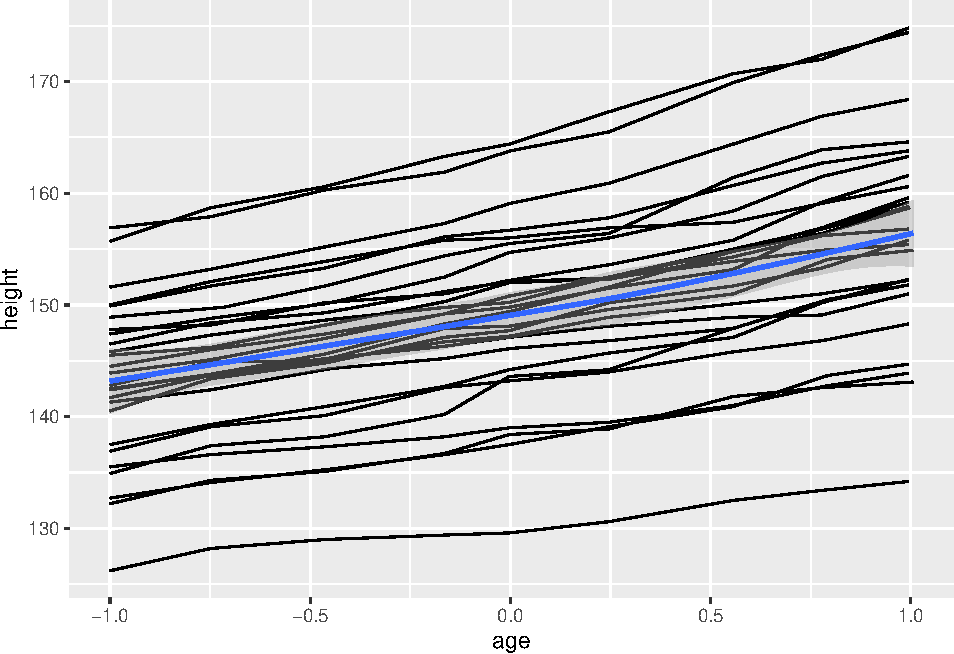
\includegraphics{Introduction-to-R,-Rstudio,-and-ggplot2_files/figure-latex/unnamed-chunk-36-1.pdf}

\begin{Shaded}
\begin{Highlighting}[]
\CommentTok{# facet is also useful for visualizing longitudinal data}
\KeywordTok{ggplot}\NormalTok{(Oxboys, }\KeywordTok{aes}\NormalTok{(age, height)) +}\StringTok{ }\KeywordTok{geom_line}\NormalTok{() +}\StringTok{ }\KeywordTok{facet_wrap}\NormalTok{(~Subject)}
\end{Highlighting}
\end{Shaded}

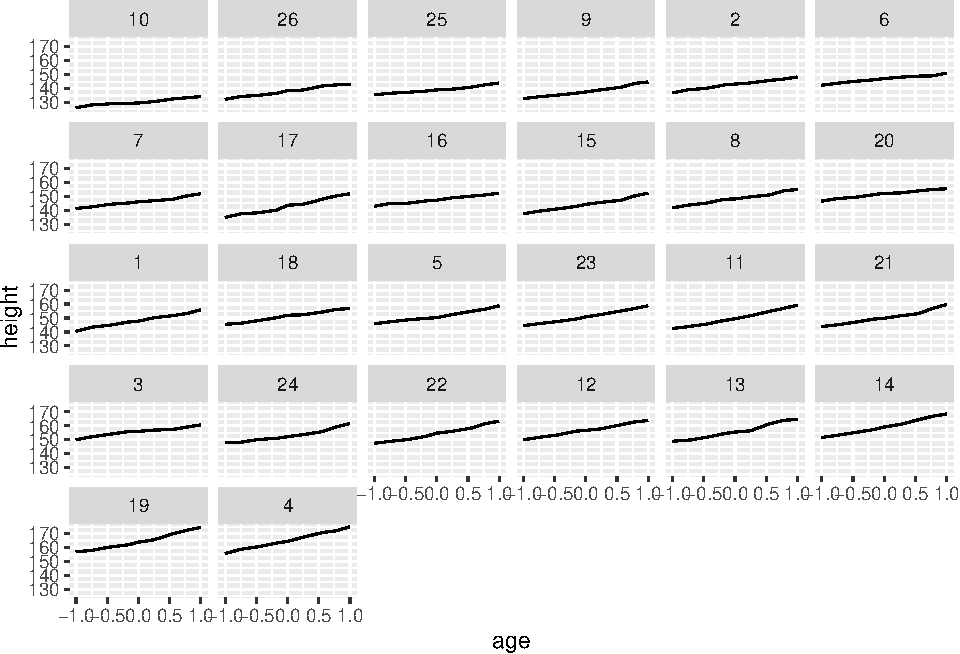
\includegraphics{Introduction-to-R,-Rstudio,-and-ggplot2_files/figure-latex/unnamed-chunk-37-1.pdf}

\section{Themes}\label{themes}

``Themes are a powerful way to \textbf{customize} the non-data
components of your plots: i.e.~titles, labels, fonts, background,
gridlines, and legends.'' More details are available at
\url{https://ggplot2.tidyverse.org/reference/theme.html}

\begin{Shaded}
\begin{Highlighting}[]
\KeywordTok{ggplot}\NormalTok{(mpg, }\KeywordTok{aes}\NormalTok{(}\DataTypeTok{x =} \NormalTok{hwy, }\DataTypeTok{y =} \NormalTok{cty)) +}\StringTok{ }\KeywordTok{geom_point}\NormalTok{() }
\end{Highlighting}
\end{Shaded}

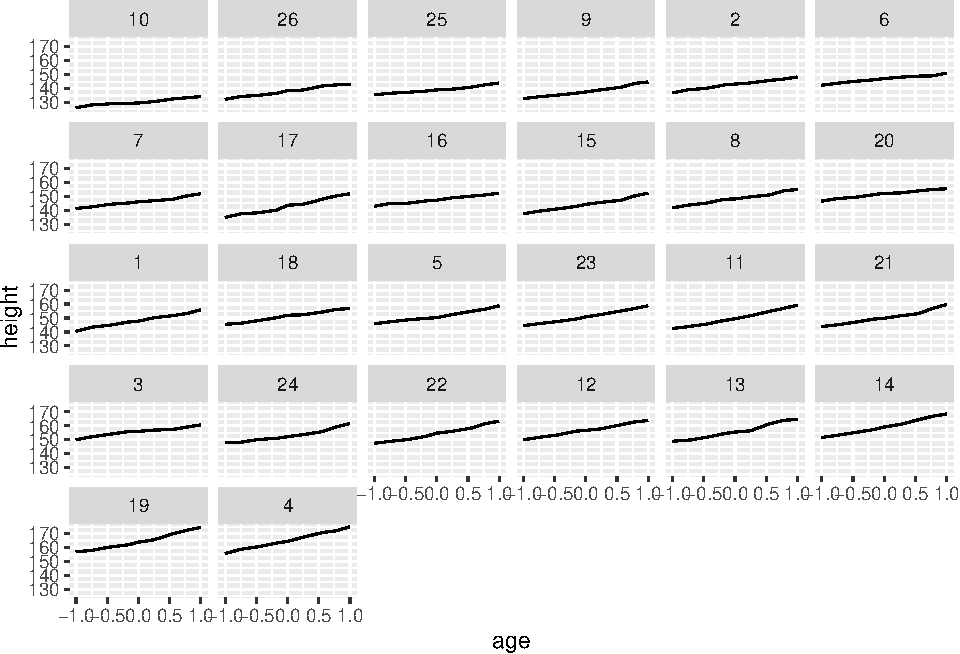
\includegraphics{Introduction-to-R,-Rstudio,-and-ggplot2_files/figure-latex/unnamed-chunk-38-1.pdf}

\begin{Shaded}
\begin{Highlighting}[]
\KeywordTok{ggplot}\NormalTok{(mpg, }\KeywordTok{aes}\NormalTok{(}\DataTypeTok{x =} \NormalTok{hwy, }\DataTypeTok{y =} \NormalTok{cty)) +}\StringTok{ }\KeywordTok{geom_point}\NormalTok{() +}\StringTok{ }\KeywordTok{theme}\NormalTok{(}\DataTypeTok{panel.background =} \KeywordTok{element_rect}\NormalTok{(}\DataTypeTok{fill =} \StringTok{"white"}\NormalTok{, }\DataTypeTok{colour =} \StringTok{"grey50"}\NormalTok{))}
\end{Highlighting}
\end{Shaded}

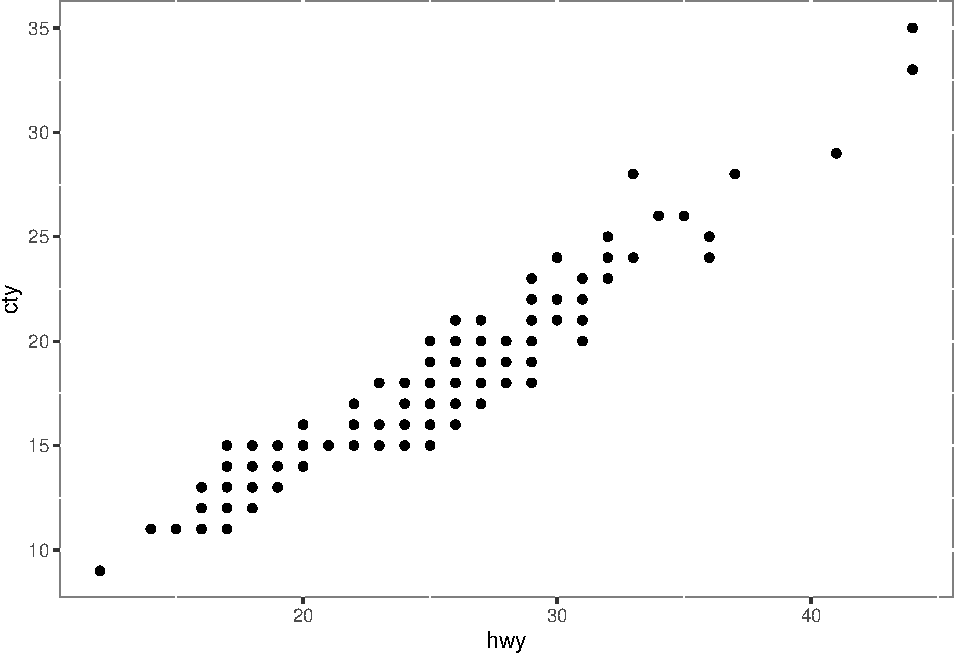
\includegraphics{Introduction-to-R,-Rstudio,-and-ggplot2_files/figure-latex/unnamed-chunk-39-1.pdf}

\begin{Shaded}
\begin{Highlighting}[]
\KeywordTok{ggplot}\NormalTok{(mpg, }\KeywordTok{aes}\NormalTok{(}\DataTypeTok{x =} \NormalTok{hwy, }\DataTypeTok{y =} \NormalTok{cty)) +}\StringTok{ }\KeywordTok{geom_point}\NormalTok{() +}\StringTok{ }\KeywordTok{theme_classic}\NormalTok{()}
\end{Highlighting}
\end{Shaded}

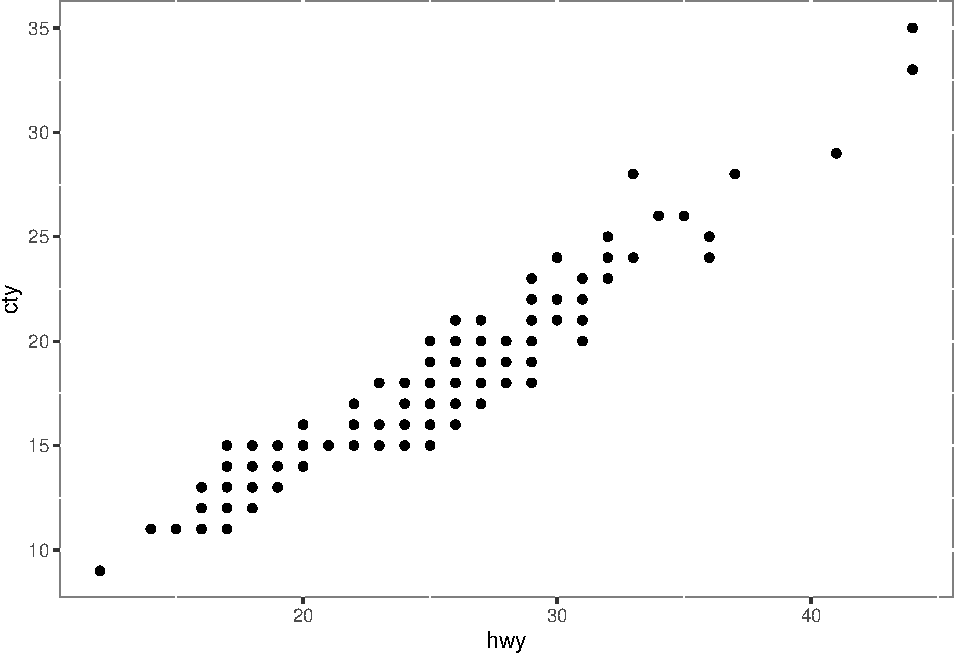
\includegraphics{Introduction-to-R,-Rstudio,-and-ggplot2_files/figure-latex/unnamed-chunk-40-1.pdf}

\section{Save a ggplot}\label{save-a-ggplot}

\begin{itemize}
\tightlist
\item
  \texttt{ggsave()} is a convenient function for saving a plot. It
  defaults to saving the \textbf{last plot} that you displayed.
\end{itemize}

\begin{Shaded}
\begin{Highlighting}[]
\KeywordTok{ggsave}\NormalTok{(}\StringTok{"mtcars.pdf"}\NormalTok{)}
\end{Highlighting}
\end{Shaded}

\begin{verbatim}
## Saving 6.5 x 4.5 in image
\end{verbatim}

\section{More resources}\label{more-resources}

\begin{itemize}
\tightlist
\item
  \texttt{ggplot2} Reference:
  \url{https://ggplot2.tidyverse.org/reference/index.html}
\item
  Many R galleries (e.g., \url{https://www.r-graph-gallery.com})
\item
  Google
\end{itemize}

\chapter{Descriptive Statistics}\label{descriptive-statistics}

\section{R functions for descriptive
statistics}\label{r-functions-for-descriptive-statistics}

\begin{Shaded}
\begin{Highlighting}[]
\CommentTok{# compute mean}
\CommentTok{# we use $ to access `price` variable in the `diamonds` dataset }
\KeywordTok{mean}\NormalTok{(diamonds$price)}
\end{Highlighting}
\end{Shaded}

\begin{verbatim}
## [1] 3932.8
\end{verbatim}

\begin{Shaded}
\begin{Highlighting}[]
\CommentTok{# compute median}
\KeywordTok{median}\NormalTok{(diamonds$price)}
\end{Highlighting}
\end{Shaded}

\begin{verbatim}
## [1] 2401
\end{verbatim}

\begin{Shaded}
\begin{Highlighting}[]
\CommentTok{# compute variance}
\KeywordTok{var}\NormalTok{(diamonds$price)}
\end{Highlighting}
\end{Shaded}

\begin{verbatim}
## [1] 15915629
\end{verbatim}

\begin{Shaded}
\begin{Highlighting}[]
\CommentTok{# compute standard deviation}
\KeywordTok{sd}\NormalTok{(diamonds$price)}
\end{Highlighting}
\end{Shaded}

\begin{verbatim}
## [1] 3989.44
\end{verbatim}

\begin{Shaded}
\begin{Highlighting}[]
\CommentTok{# summary of a data frame}
\KeywordTok{summary}\NormalTok{(diamonds)}
\end{Highlighting}
\end{Shaded}

\begin{verbatim}
##      carat               cut        color        clarity     
##  Min.   :0.2000   Fair     : 1610   D: 6775   SI1    :13065  
##  1st Qu.:0.4000   Good     : 4906   E: 9797   VS2    :12258  
##  Median :0.7000   Very Good:12082   F: 9542   SI2    : 9194  
##  Mean   :0.7979   Premium  :13791   G:11292   VS1    : 8171  
##  3rd Qu.:1.0400   Ideal    :21551   H: 8304   VVS2   : 5066  
##  Max.   :5.0100                     I: 5422   VVS1   : 3655  
##                                     J: 2808   (Other): 2531  
##      depth           table           price             x         
##  Min.   :43.00   Min.   :43.00   Min.   :  326   Min.   : 0.000  
##  1st Qu.:61.00   1st Qu.:56.00   1st Qu.:  950   1st Qu.: 4.710  
##  Median :61.80   Median :57.00   Median : 2401   Median : 5.700  
##  Mean   :61.75   Mean   :57.46   Mean   : 3933   Mean   : 5.731  
##  3rd Qu.:62.50   3rd Qu.:59.00   3rd Qu.: 5324   3rd Qu.: 6.540  
##  Max.   :79.00   Max.   :95.00   Max.   :18823   Max.   :10.740  
##                                                                  
##        y                z         
##  Min.   : 0.000   Min.   : 0.000  
##  1st Qu.: 4.720   1st Qu.: 2.910  
##  Median : 5.710   Median : 3.530  
##  Mean   : 5.735   Mean   : 3.539  
##  3rd Qu.: 6.540   3rd Qu.: 4.040  
##  Max.   :58.900   Max.   :31.800  
## 
\end{verbatim}

\section{qplot()}\label{qplot}

\texttt{qplot()}, short for \textbf{quick plot} is a function in the
\texttt{ggplot2} package. qplot makes it easy to produce complex plots,
often requiring several lines of code using other plotting systems,
\textbf{in one line}.

\section{Scatterplots}\label{scatterplots}

\begin{Shaded}
\begin{Highlighting}[]
\KeywordTok{ggplot}\NormalTok{(}\DataTypeTok{data =} \NormalTok{mpg, }\KeywordTok{aes}\NormalTok{(}\DataTypeTok{x =} \NormalTok{displ, }\DataTypeTok{y =} \NormalTok{hwy)) +}\StringTok{ }\KeywordTok{geom_point}\NormalTok{()}
\end{Highlighting}
\end{Shaded}

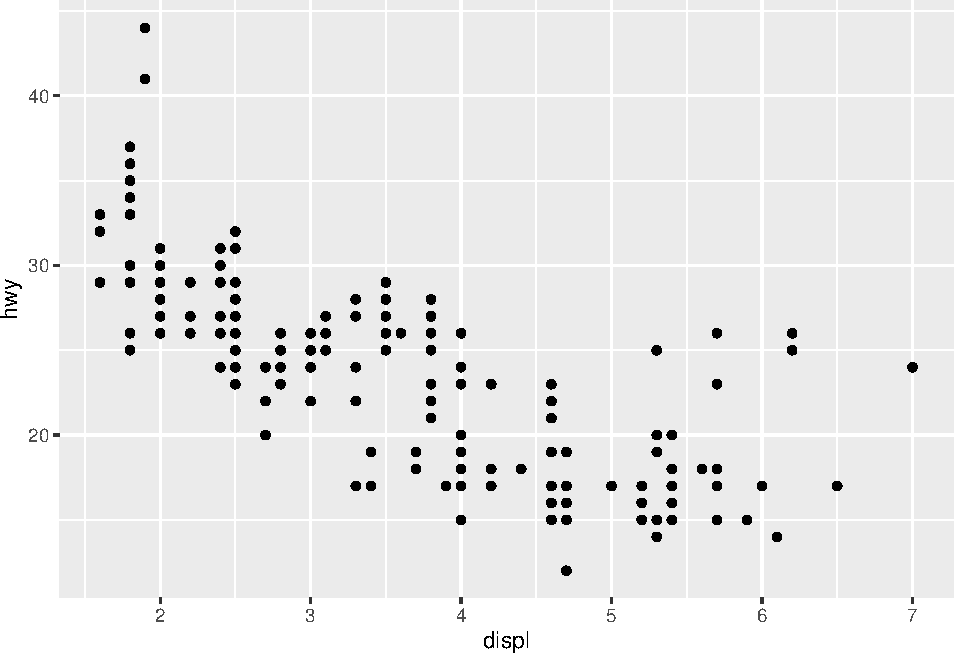
\includegraphics{Introduction-to-R,-Rstudio,-and-ggplot2_files/figure-latex/unnamed-chunk-47-1.pdf}

\begin{Shaded}
\begin{Highlighting}[]
\KeywordTok{qplot}\NormalTok{(displ, hwy, }\DataTypeTok{data =} \NormalTok{mpg)}
\end{Highlighting}
\end{Shaded}

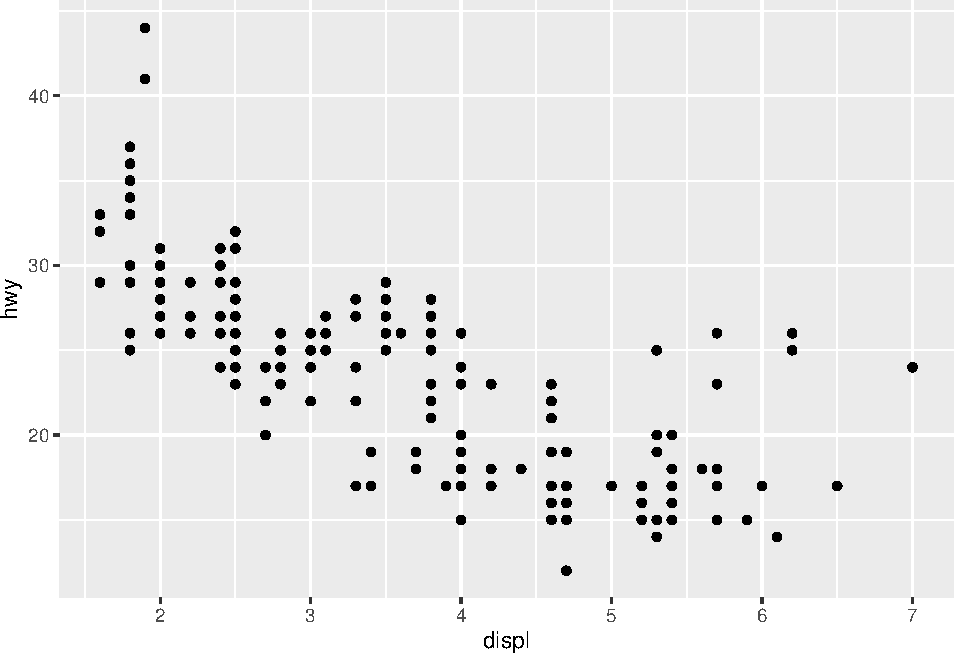
\includegraphics{Introduction-to-R,-Rstudio,-and-ggplot2_files/figure-latex/unnamed-chunk-48-1.pdf}

\begin{Shaded}
\begin{Highlighting}[]
\KeywordTok{ggplot}\NormalTok{(}\DataTypeTok{data =} \NormalTok{mpg, }\KeywordTok{aes}\NormalTok{(}\DataTypeTok{x =} \NormalTok{displ, }\DataTypeTok{y =} \NormalTok{hwy, }\DataTypeTok{color =} \NormalTok{class)) +}\StringTok{ }\KeywordTok{geom_point}\NormalTok{()}
\end{Highlighting}
\end{Shaded}

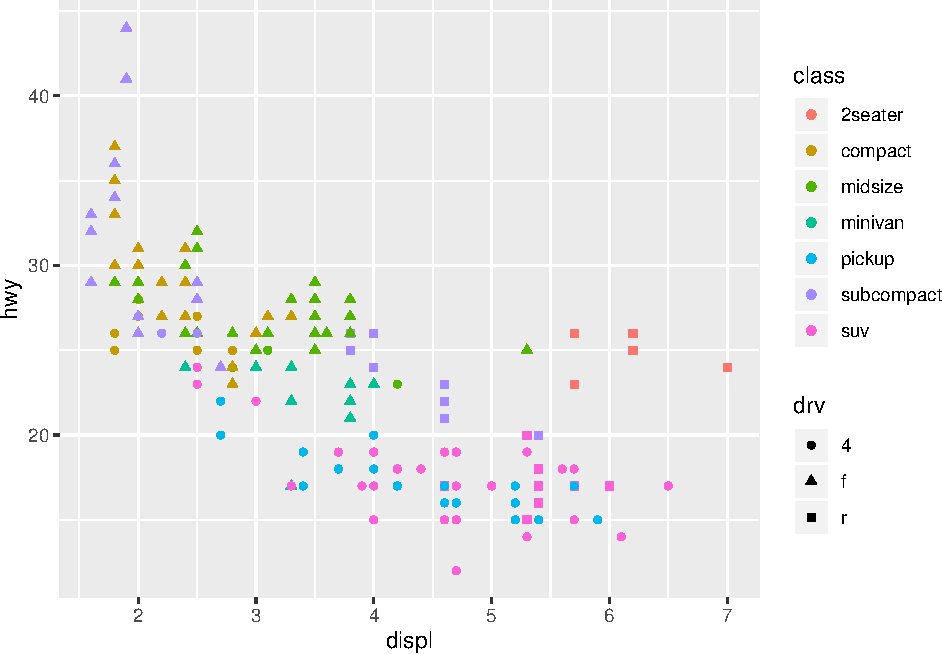
\includegraphics{Introduction-to-R,-Rstudio,-and-ggplot2_files/figure-latex/unnamed-chunk-49-1.pdf}

\begin{Shaded}
\begin{Highlighting}[]
\KeywordTok{qplot}\NormalTok{(displ, hwy, }\DataTypeTok{data =} \NormalTok{mpg, }\DataTypeTok{color =} \NormalTok{class)}
\end{Highlighting}
\end{Shaded}

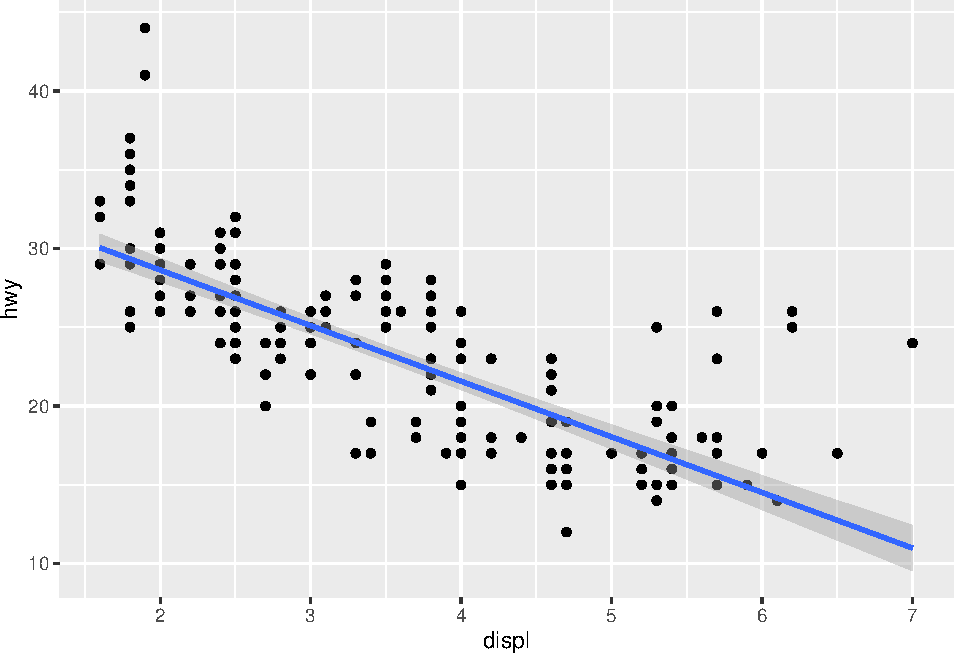
\includegraphics{Introduction-to-R,-Rstudio,-and-ggplot2_files/figure-latex/unnamed-chunk-50-1.pdf}

\begin{Shaded}
\begin{Highlighting}[]
\KeywordTok{ggplot}\NormalTok{(}\DataTypeTok{data =} \NormalTok{mpg, }\KeywordTok{aes}\NormalTok{(}\DataTypeTok{x =} \NormalTok{displ, }\DataTypeTok{y =} \NormalTok{hwy, }\DataTypeTok{color =} \NormalTok{class, }\DataTypeTok{shape =} \NormalTok{drv)) +}\StringTok{ }\KeywordTok{geom_point}\NormalTok{()}
\end{Highlighting}
\end{Shaded}

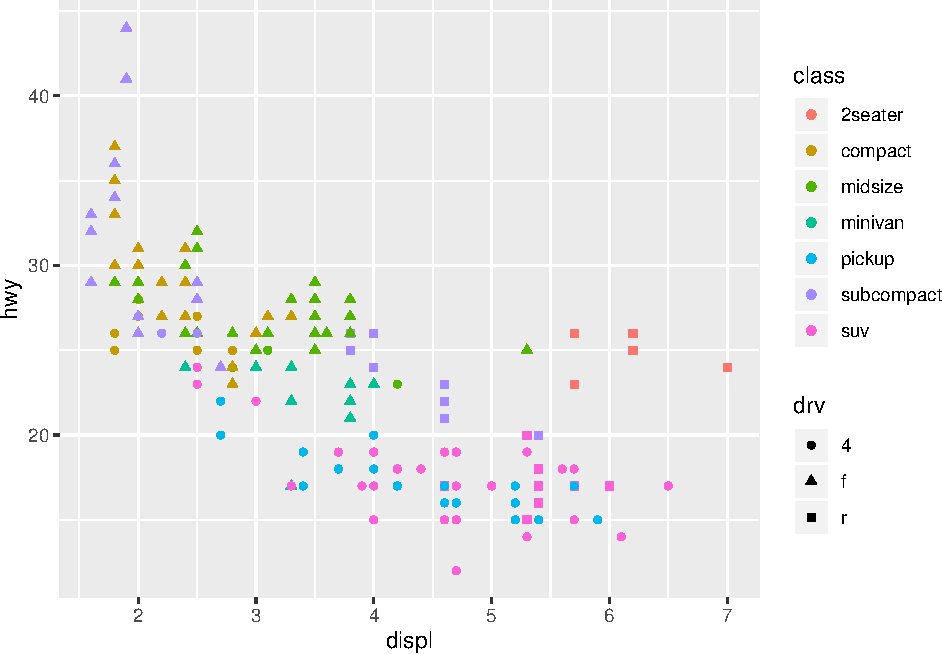
\includegraphics{Introduction-to-R,-Rstudio,-and-ggplot2_files/figure-latex/unnamed-chunk-51-1.pdf}

\begin{Shaded}
\begin{Highlighting}[]
\KeywordTok{qplot}\NormalTok{(displ, hwy, }\DataTypeTok{data =} \NormalTok{mpg, }\DataTypeTok{color =} \NormalTok{class, }\DataTypeTok{shape =} \NormalTok{drv)}
\end{Highlighting}
\end{Shaded}

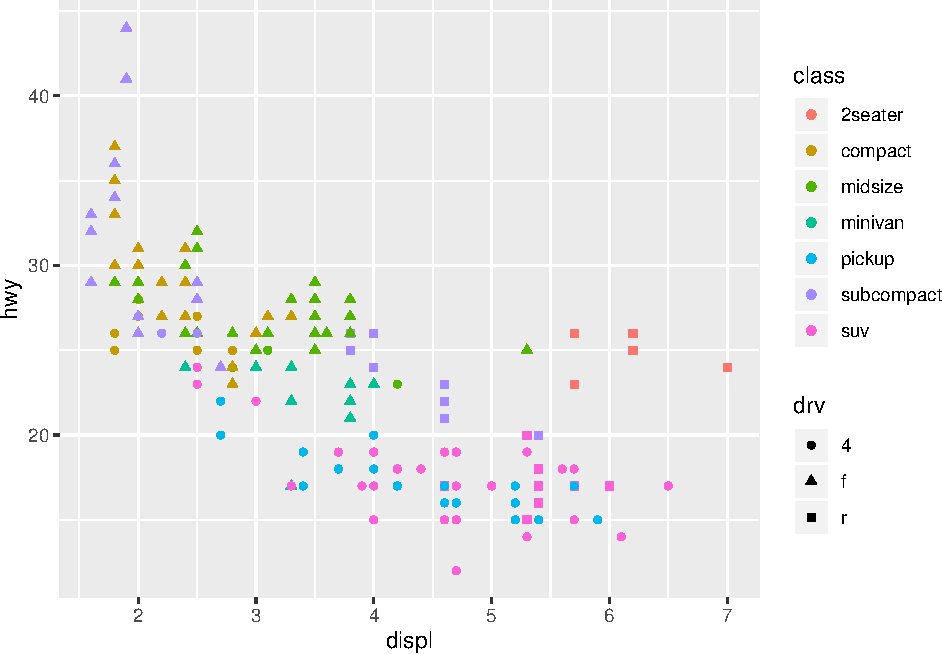
\includegraphics{Introduction-to-R,-Rstudio,-and-ggplot2_files/figure-latex/unnamed-chunk-52-1.pdf}

\begin{Shaded}
\begin{Highlighting}[]
\KeywordTok{ggplot}\NormalTok{(}\DataTypeTok{data =} \NormalTok{mpg, }\KeywordTok{aes}\NormalTok{(}\DataTypeTok{x =} \NormalTok{displ, }\DataTypeTok{y =} \NormalTok{hwy)) +}\StringTok{ }\KeywordTok{geom_point}\NormalTok{() +}\StringTok{ }\KeywordTok{geom_smooth}\NormalTok{(}\DataTypeTok{method =} \StringTok{"lm"}\NormalTok{)}
\end{Highlighting}
\end{Shaded}

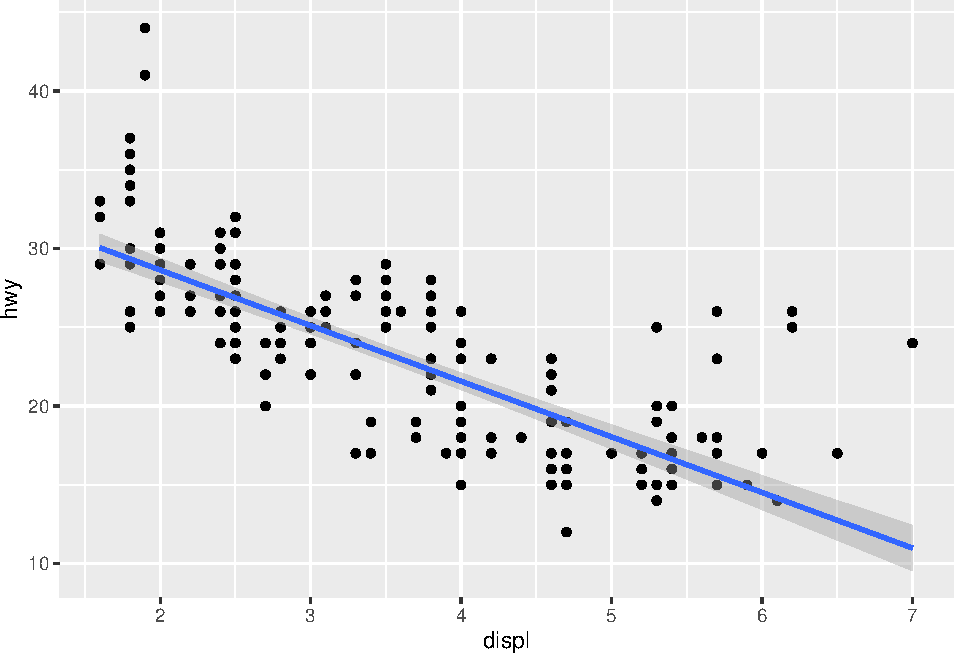
\includegraphics{Introduction-to-R,-Rstudio,-and-ggplot2_files/figure-latex/unnamed-chunk-53-1.pdf}

\begin{Shaded}
\begin{Highlighting}[]
\KeywordTok{qplot}\NormalTok{(displ, hwy, }\DataTypeTok{data =} \NormalTok{mpg, }\DataTypeTok{geom =} \KeywordTok{c}\NormalTok{(}\StringTok{"point"}\NormalTok{, }\StringTok{"smooth"}\NormalTok{)) }
\end{Highlighting}
\end{Shaded}

\begin{verbatim}
## `geom_smooth()` using method = 'loess' and formula 'y ~ x'
\end{verbatim}

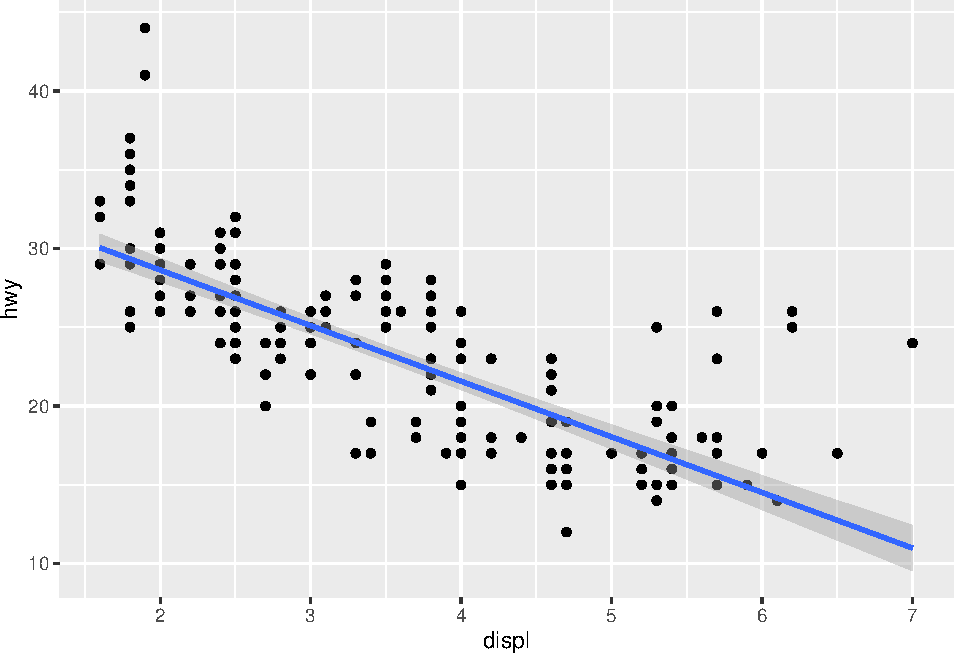
\includegraphics{Introduction-to-R,-Rstudio,-and-ggplot2_files/figure-latex/unnamed-chunk-54-1.pdf}

\section{Histogram}\label{histogram}

\begin{Shaded}
\begin{Highlighting}[]
\KeywordTok{ggplot}\NormalTok{(}\DataTypeTok{data =} \NormalTok{diamonds, }\KeywordTok{aes}\NormalTok{(}\DataTypeTok{x =} \NormalTok{carat)) +}\StringTok{ }\KeywordTok{geom_histogram}\NormalTok{()}
\end{Highlighting}
\end{Shaded}

\begin{verbatim}
## `stat_bin()` using `bins = 30`. Pick better value with `binwidth`.
\end{verbatim}

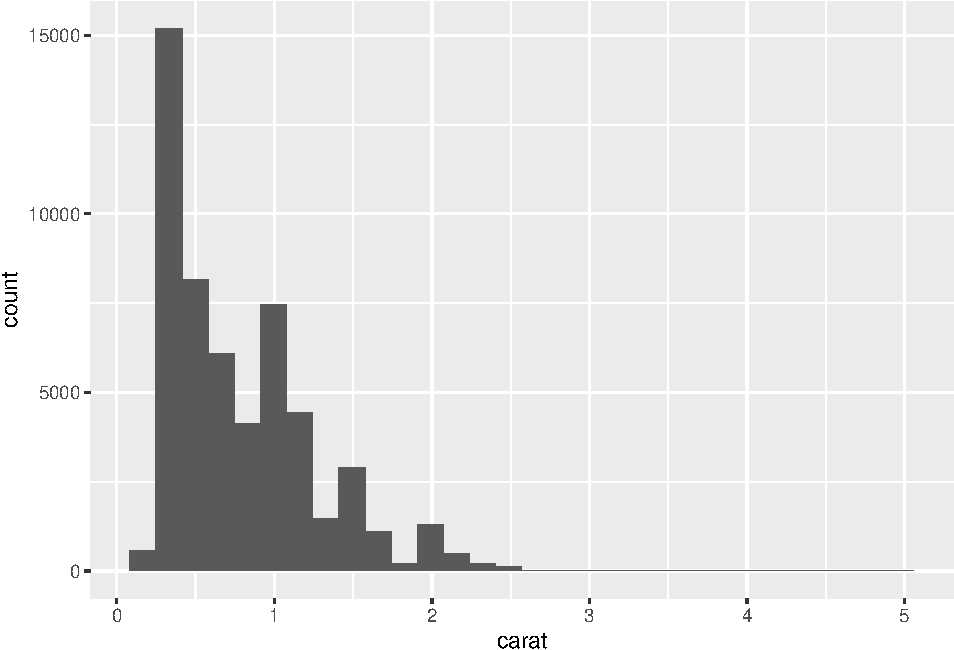
\includegraphics{Introduction-to-R,-Rstudio,-and-ggplot2_files/figure-latex/unnamed-chunk-55-1.pdf}

\begin{Shaded}
\begin{Highlighting}[]
\KeywordTok{qplot}\NormalTok{(carat, }\DataTypeTok{data =} \NormalTok{diamonds, }\DataTypeTok{geom =} \StringTok{"histogram"}\NormalTok{)}
\end{Highlighting}
\end{Shaded}

\begin{verbatim}
## `stat_bin()` using `bins = 30`. Pick better value with `binwidth`.
\end{verbatim}

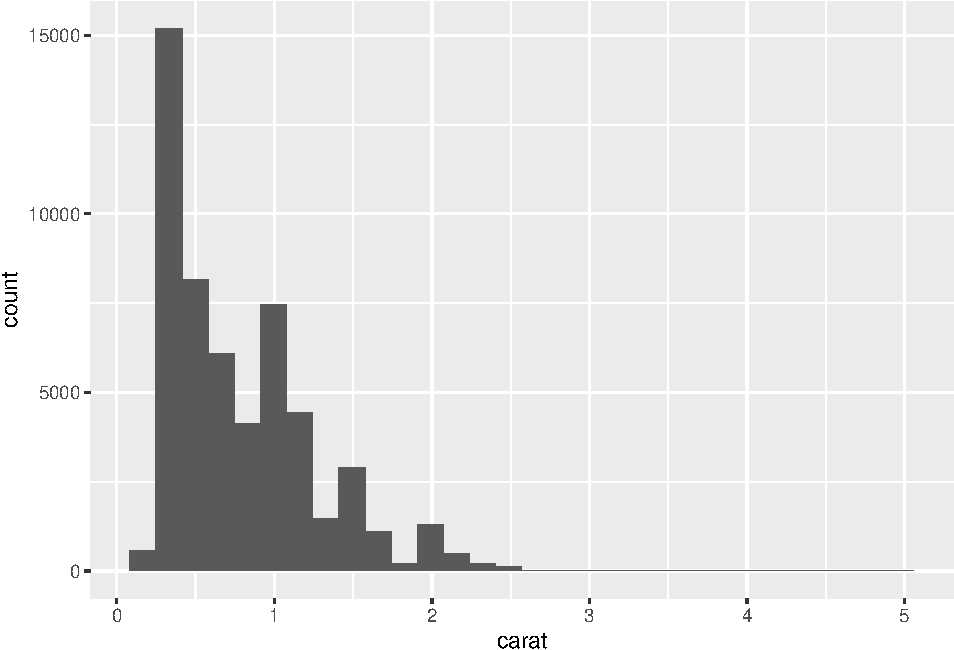
\includegraphics{Introduction-to-R,-Rstudio,-and-ggplot2_files/figure-latex/unnamed-chunk-56-1.pdf}

\begin{Shaded}
\begin{Highlighting}[]
\KeywordTok{ggplot}\NormalTok{(}\DataTypeTok{data =} \NormalTok{diamonds, }\KeywordTok{aes}\NormalTok{(}\DataTypeTok{x =} \NormalTok{carat)) +}\StringTok{ }\KeywordTok{geom_histogram}\NormalTok{(}\DataTypeTok{binwidth =} \FloatTok{0.05}\NormalTok{) +}\StringTok{ }\KeywordTok{xlim}\NormalTok{(}\KeywordTok{c}\NormalTok{(}\DecValTok{0}\NormalTok{,}\DecValTok{3}\NormalTok{))}
\end{Highlighting}
\end{Shaded}

\begin{verbatim}
## Warning: Removed 32 rows containing non-finite values (stat_bin).
\end{verbatim}

\begin{verbatim}
## Warning: Removed 2 rows containing missing values (geom_bar).
\end{verbatim}

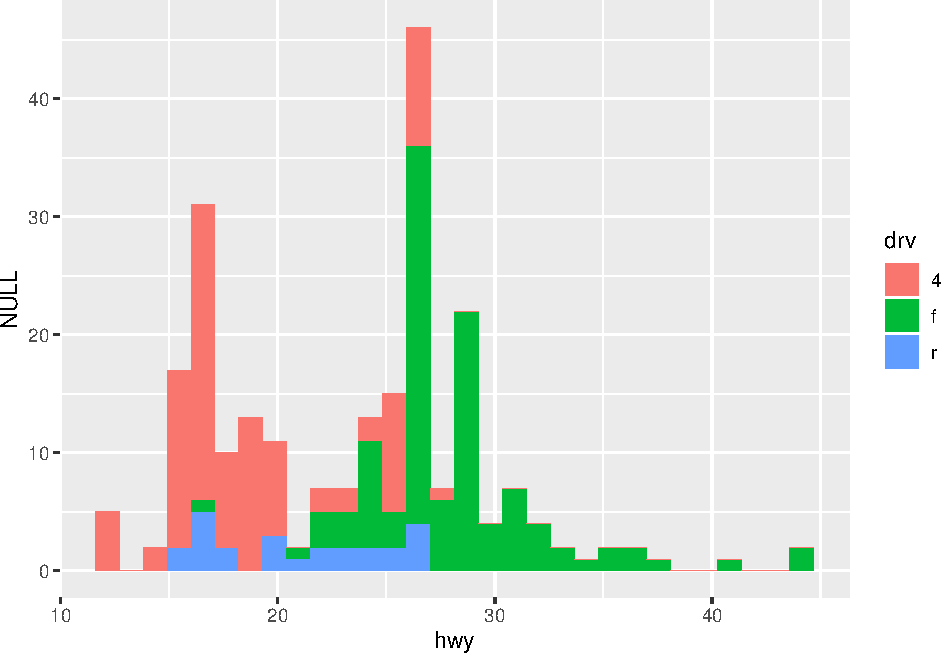
\includegraphics{Introduction-to-R,-Rstudio,-and-ggplot2_files/figure-latex/unnamed-chunk-57-1.pdf}

\begin{Shaded}
\begin{Highlighting}[]
\KeywordTok{qplot}\NormalTok{(carat, }\DataTypeTok{data =} \NormalTok{diamonds, }\DataTypeTok{geom =} \StringTok{"histogram"}\NormalTok{, }\DataTypeTok{binwidth =} \FloatTok{0.05}\NormalTok{, }\DataTypeTok{xlim =} \KeywordTok{c}\NormalTok{(}\DecValTok{0}\NormalTok{,}\DecValTok{3}\NormalTok{))}
\end{Highlighting}
\end{Shaded}

\begin{verbatim}
## Warning: Removed 32 rows containing non-finite values (stat_bin).
\end{verbatim}

\begin{verbatim}
## Warning: Removed 2 rows containing missing values (geom_bar).
\end{verbatim}

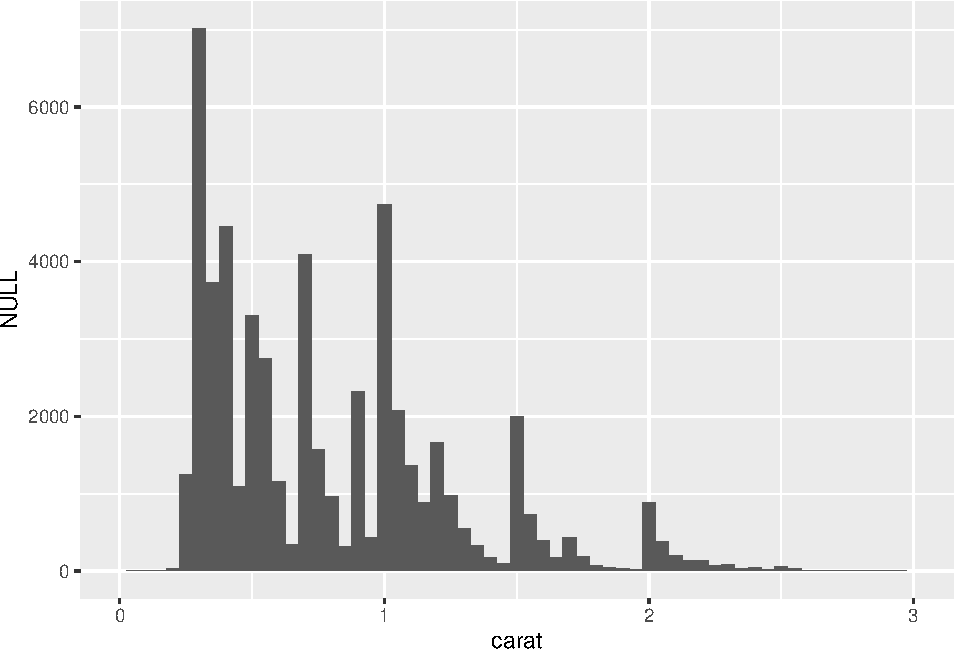
\includegraphics{Introduction-to-R,-Rstudio,-and-ggplot2_files/figure-latex/unnamed-chunk-58-1.pdf}

\begin{Shaded}
\begin{Highlighting}[]
\KeywordTok{ggplot}\NormalTok{(}\DataTypeTok{data =} \NormalTok{mpg, }\KeywordTok{aes}\NormalTok{(}\DataTypeTok{x =} \NormalTok{hwy, }\DataTypeTok{fill =} \NormalTok{drv)) +}\StringTok{ }\KeywordTok{geom_histogram}\NormalTok{() }
\end{Highlighting}
\end{Shaded}

\begin{verbatim}
## `stat_bin()` using `bins = 30`. Pick better value with `binwidth`.
\end{verbatim}

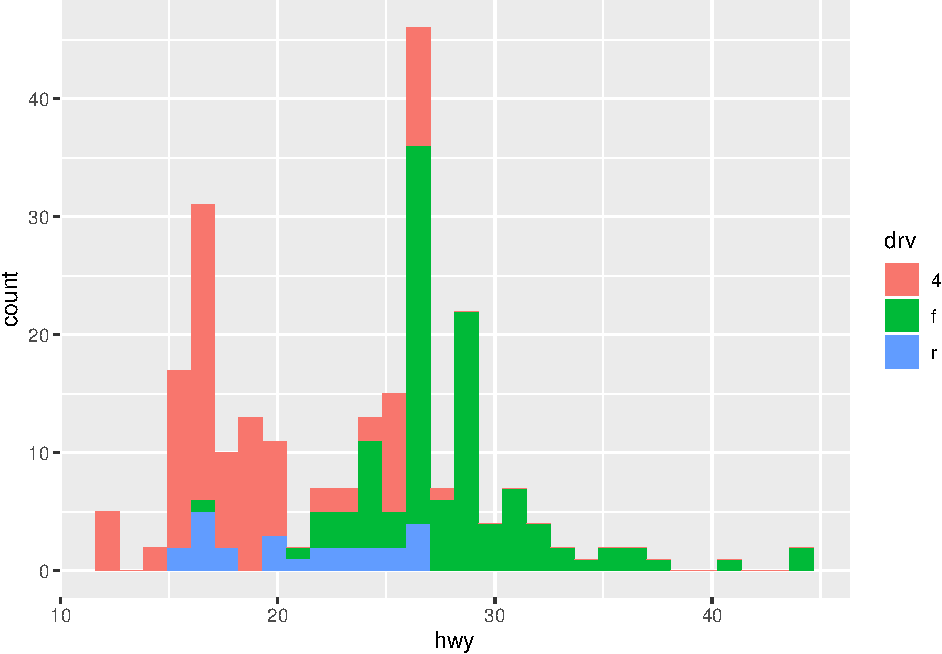
\includegraphics{Introduction-to-R,-Rstudio,-and-ggplot2_files/figure-latex/unnamed-chunk-59-1.pdf}

\begin{Shaded}
\begin{Highlighting}[]
\KeywordTok{qplot}\NormalTok{(hwy, }\DataTypeTok{data =} \NormalTok{mpg, }\DataTypeTok{geom =} \StringTok{"histogram"}\NormalTok{, }\DataTypeTok{fill =} \NormalTok{drv)}
\end{Highlighting}
\end{Shaded}

\begin{verbatim}
## `stat_bin()` using `bins = 30`. Pick better value with `binwidth`.
\end{verbatim}

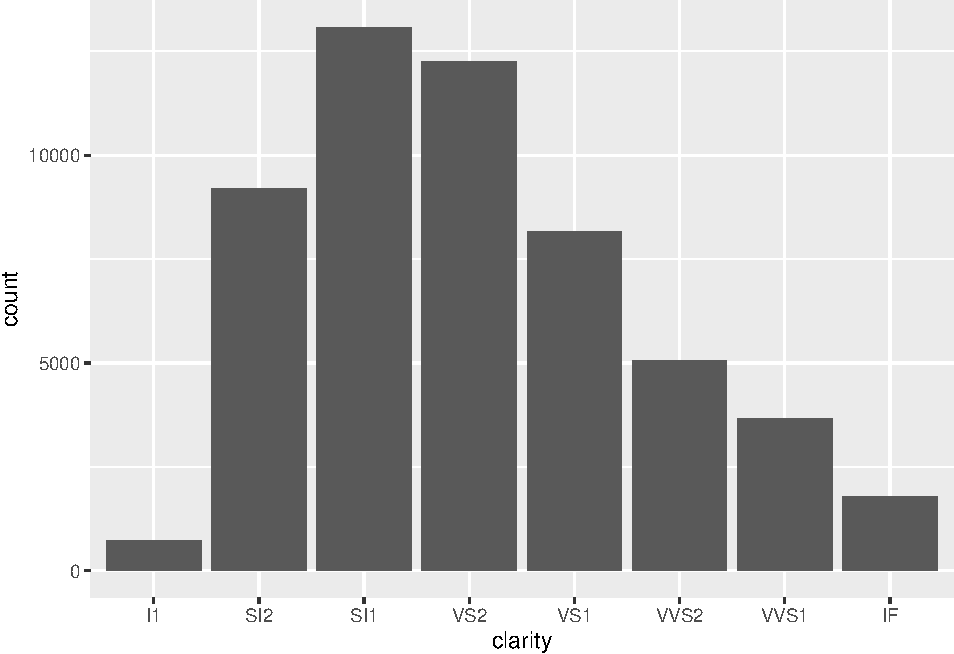
\includegraphics{Introduction-to-R,-Rstudio,-and-ggplot2_files/figure-latex/unnamed-chunk-60-1.pdf}

\section{Density plots}\label{density-plots}

\begin{Shaded}
\begin{Highlighting}[]
\KeywordTok{ggplot}\NormalTok{(}\DataTypeTok{data =} \NormalTok{diamonds, }\KeywordTok{aes}\NormalTok{(}\DataTypeTok{x =} \NormalTok{carat, }\DataTypeTok{color =} \NormalTok{color)) +}\StringTok{ }\KeywordTok{geom_density}\NormalTok{() }
\end{Highlighting}
\end{Shaded}

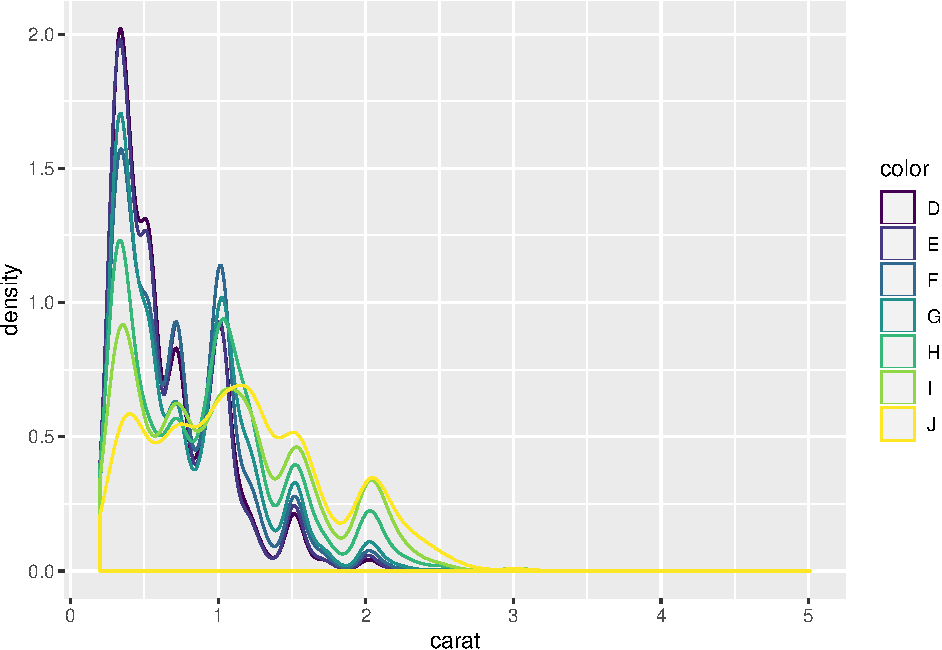
\includegraphics{Introduction-to-R,-Rstudio,-and-ggplot2_files/figure-latex/unnamed-chunk-61-1.pdf}

\begin{Shaded}
\begin{Highlighting}[]
\KeywordTok{qplot}\NormalTok{(carat, }\DataTypeTok{data =} \NormalTok{diamonds, }\DataTypeTok{geom =} \StringTok{"density"}\NormalTok{, }\DataTypeTok{color =} \NormalTok{color)}
\end{Highlighting}
\end{Shaded}

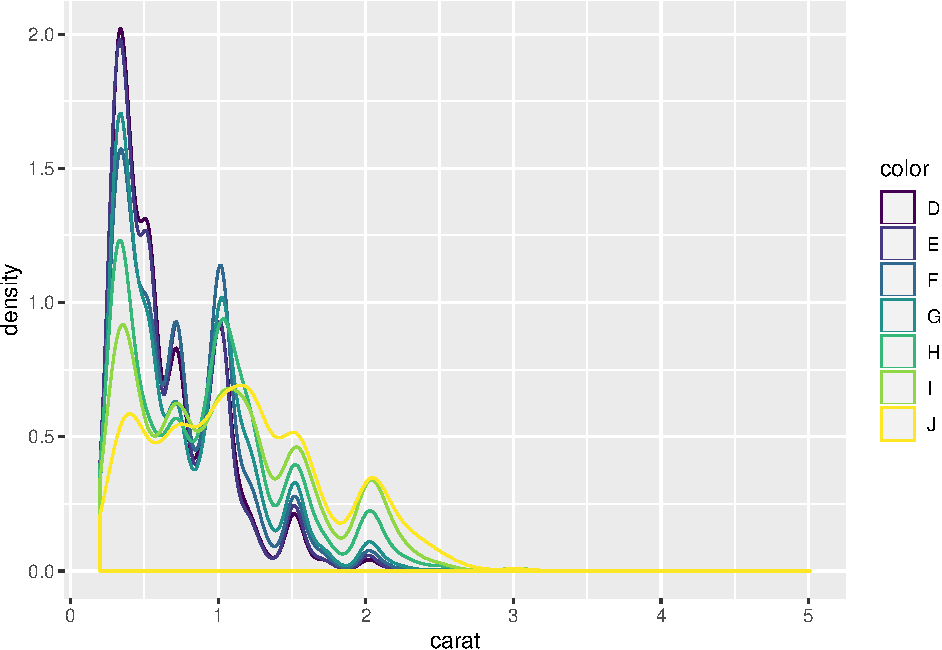
\includegraphics{Introduction-to-R,-Rstudio,-and-ggplot2_files/figure-latex/unnamed-chunk-62-1.pdf}

\section{Barplots}\label{barplots}

\begin{Shaded}
\begin{Highlighting}[]
\KeywordTok{ggplot}\NormalTok{(}\DataTypeTok{data =} \NormalTok{diamonds, }\KeywordTok{aes}\NormalTok{(}\DataTypeTok{x =} \NormalTok{clarity)) +}\StringTok{ }\KeywordTok{geom_bar}\NormalTok{() }
\end{Highlighting}
\end{Shaded}

\includegraphics{Introduction-to-R,-Rstudio,-and-ggplot2_files/figure-latex/unnamed-chunk-63-1.pdf}

\begin{Shaded}
\begin{Highlighting}[]
\KeywordTok{qplot}\NormalTok{(clarity, }\DataTypeTok{data =} \NormalTok{diamonds, }\DataTypeTok{geom =} \StringTok{"bar"}\NormalTok{)}
\end{Highlighting}
\end{Shaded}

\includegraphics{Introduction-to-R,-Rstudio,-and-ggplot2_files/figure-latex/unnamed-chunk-64-1.pdf}

\begin{Shaded}
\begin{Highlighting}[]
\KeywordTok{ggplot}\NormalTok{(}\DataTypeTok{data =} \NormalTok{diamonds, }\KeywordTok{aes}\NormalTok{(}\DataTypeTok{x =} \NormalTok{clarity, }\DataTypeTok{fill =} \NormalTok{cut)) +}\StringTok{ }\KeywordTok{geom_bar}\NormalTok{() }
\end{Highlighting}
\end{Shaded}

\includegraphics{Introduction-to-R,-Rstudio,-and-ggplot2_files/figure-latex/unnamed-chunk-65-1.pdf}

\begin{Shaded}
\begin{Highlighting}[]
\KeywordTok{qplot}\NormalTok{(clarity, }\DataTypeTok{data =} \NormalTok{diamonds, }\DataTypeTok{geom =} \StringTok{"bar"}\NormalTok{, }\DataTypeTok{fill =} \NormalTok{cut)}
\end{Highlighting}
\end{Shaded}

\includegraphics{Introduction-to-R,-Rstudio,-and-ggplot2_files/figure-latex/unnamed-chunk-66-1.pdf}

\section{Boxplots}\label{boxplots}

\begin{Shaded}
\begin{Highlighting}[]
\KeywordTok{ggplot}\NormalTok{(}\DataTypeTok{data =} \NormalTok{diamonds, }\KeywordTok{aes}\NormalTok{(}\DataTypeTok{y =} \NormalTok{price)) +}\StringTok{ }\KeywordTok{geom_boxplot}\NormalTok{() }
\end{Highlighting}
\end{Shaded}

\includegraphics{Introduction-to-R,-Rstudio,-and-ggplot2_files/figure-latex/unnamed-chunk-67-1.pdf}

\begin{Shaded}
\begin{Highlighting}[]
\KeywordTok{qplot}\NormalTok{(}\DataTypeTok{y =} \NormalTok{price, }\DataTypeTok{data =} \NormalTok{diamonds, }\DataTypeTok{geom =} \StringTok{"boxplot"}\NormalTok{)}
\end{Highlighting}
\end{Shaded}

\includegraphics{Introduction-to-R,-Rstudio,-and-ggplot2_files/figure-latex/unnamed-chunk-68-1.pdf}

\begin{Shaded}
\begin{Highlighting}[]
\KeywordTok{ggplot}\NormalTok{(}\DataTypeTok{data =} \NormalTok{diamonds, }\KeywordTok{aes}\NormalTok{(}\DataTypeTok{x =} \NormalTok{cut, }\DataTypeTok{y =} \NormalTok{price)) +}\StringTok{ }\KeywordTok{geom_boxplot}\NormalTok{() }
\end{Highlighting}
\end{Shaded}

\includegraphics{Introduction-to-R,-Rstudio,-and-ggplot2_files/figure-latex/unnamed-chunk-69-1.pdf}

\section{Faceting}\label{faceting}

\begin{Shaded}
\begin{Highlighting}[]
\KeywordTok{ggplot}\NormalTok{(}\DataTypeTok{data =} \NormalTok{diamonds, }\KeywordTok{aes}\NormalTok{(}\DataTypeTok{x =} \NormalTok{carat, }\DataTypeTok{y =} \NormalTok{price)) +}\StringTok{ }\KeywordTok{geom_point}\NormalTok{() +}\StringTok{ }\KeywordTok{facet_grid}\NormalTok{(cut ~}\StringTok{ }\NormalTok{color)}
\end{Highlighting}
\end{Shaded}

\includegraphics{Introduction-to-R,-Rstudio,-and-ggplot2_files/figure-latex/unnamed-chunk-70-1.pdf}

\begin{Shaded}
\begin{Highlighting}[]
\KeywordTok{qplot}\NormalTok{(carat, price, }\DataTypeTok{data =} \NormalTok{diamonds, }\DataTypeTok{facets =} \NormalTok{cut ~}\StringTok{ }\NormalTok{color)}
\end{Highlighting}
\end{Shaded}

\includegraphics{Introduction-to-R,-Rstudio,-and-ggplot2_files/figure-latex/unnamed-chunk-71-1.pdf}

\section{\texorpdfstring{The \texttt{corrplot}
Package}{The corrplot Package}}\label{the-corrplot-package}

\begin{itemize}
\tightlist
\item
  \url{https://cran.r-project.org/web/packages/corrplot/vignettes/corrplot-intro.html}
\item
  ``The corrplot package is a graphical display of a \textbf{correlation
  matrix}, confidence interval. It also contains some algorithms to do
  matrix reordering. In addition, corrplot is good at details, including
  choosing color, text labels, color labels, layout, etc.''
\end{itemize}

\begin{Shaded}
\begin{Highlighting}[]
\KeywordTok{library}\NormalTok{(corrplot)}
\end{Highlighting}
\end{Shaded}

\begin{Shaded}
\begin{Highlighting}[]
\KeywordTok{corrplot.mixed}\NormalTok{(}\KeywordTok{cor}\NormalTok{(mtcars))}
\end{Highlighting}
\end{Shaded}

\includegraphics{Introduction-to-R,-Rstudio,-and-ggplot2_files/figure-latex/unnamed-chunk-73-1.pdf}

\chapter{Exercise}\label{exercise-3}

\begin{itemize}
\tightlist
\item
  Exercise 1: \texttt{midwest} is a dataset in \texttt{ggplot2}, and
  contains demographic information of midwest counties. Replicate the
  following scatterplot as close as you can. The variable for the
  x-axis, y-axis, color aesthetic, size aesthetic are \texttt{area},
  \texttt{poptotal}, \texttt{state}, and \texttt{popdensity}.
\end{itemize}

\begin{figure}[htbp]
\centering
\includegraphics{practice1.png}
\caption{}
\end{figure}

\begin{itemize}
\tightlist
\item
  Excercise 2: Replicate the following barplot using the \texttt{mpg}
  dataset. Use
  \texttt{theme(axis.text.x\ =\ element\_text(angle=65,\ vjust=0.6))}.
  Check why we need this theme by plotting with and without this theme.
  You also need \texttt{width\ =\ 0.5} option in a geom to have more
  space between bar.
\end{itemize}

\begin{figure}[htbp]
\centering
\includegraphics{practice2.png}
\caption{}
\end{figure}

\chapter{Base R}\label{base-r}

\section{Topics}\label{topics}

\begin{itemize}
\tightlist
\item
  R Objects and Variables
\item
  Data Structure
\item
  Sub-Setting
\item
  Functions
\item
  Control Flow (if, for, while)
\end{itemize}

\section{Further reading}\label{further-reading}

\begin{itemize}
\tightlist
\item
  Wickham, H. (2014). Advanced R. Chapman and Hall/CRC
  (\url{http://adv-r.had.co.nz})

  \begin{itemize}
  \tightlist
  \item
    This is a nice book to read after you become comfortable in base R
    (not required in this course)
  \end{itemize}
\end{itemize}

\section{Interaction with R}\label{interaction-with-r}

\begin{itemize}
\tightlist
\item
  R Console: for easy interactive exploration of ideas
\item
  R Script file (.R): for sequence of R commands
\item
  R markdown (.Rmd): for reproducible and dynamic reports
\end{itemize}

\section{R Objects and Variables}\label{r-objects-and-variables}

\begin{itemize}
\tightlist
\item
  \textbf{Everything in R is stored as an object}, which is associated
  with a variable name.
\item
  An object is a technical terminology defined in \textbf{Object
  Oriented Programming (OOP)}. (OOP is an important concept but not in
  this class)
\item
  A variable name can be assigned to an object using the
  \textbf{assignment operator}.
\end{itemize}

\begin{Shaded}
\begin{Highlighting}[]
\CommentTok{# store a number to a variable named `a`}
\NormalTok{a <-}\StringTok{ }\FloatTok{0.2}
\end{Highlighting}
\end{Shaded}

\begin{Shaded}
\begin{Highlighting}[]
\CommentTok{# print a}
\NormalTok{a}
\end{Highlighting}
\end{Shaded}

\begin{verbatim}
## [1] 0.2
\end{verbatim}

\begin{Shaded}
\begin{Highlighting}[]
\CommentTok{# store a vector to a variable named `b`}
\NormalTok{b <-}\StringTok{ }\KeywordTok{c}\NormalTok{(}\DecValTok{1}\NormalTok{,}\DecValTok{4}\NormalTok{,}\DecValTok{9}\NormalTok{)}
\end{Highlighting}
\end{Shaded}

\begin{Shaded}
\begin{Highlighting}[]
\CommentTok{# print b}
\NormalTok{b}
\end{Highlighting}
\end{Shaded}

\begin{verbatim}
## [1] 1 4 9
\end{verbatim}

\begin{Shaded}
\begin{Highlighting}[]
\NormalTok{z <-}\StringTok{ }\DecValTok{5}
\NormalTok{i <-}\StringTok{ }\NormalTok{(z *}\StringTok{ }\DecValTok{2} \NormalTok{+}\StringTok{ }\DecValTok{45}\NormalTok{)/}\DecValTok{2}
\NormalTok{i}
\end{Highlighting}
\end{Shaded}

\begin{verbatim}
## [1] 27.5
\end{verbatim}

\begin{itemize}
\tightlist
\item
  We can think of the assignment operation as ``\textbf{evaluate}
  whatever is given on the \textbf{right side} of the operator, and
  assign (store) the result (an object of some type) of this evaluation
  in the variable whose name is given on the \textbf{left side}
\end{itemize}

\section{Data Structure}\label{data-structure}

\begin{itemize}
\tightlist
\item
  R has \textbf{base data structures}.
\item
  Almost all other objects are built upon base data structures.
\item
  R base data structures can be organized by their dimensionality:
\end{itemize}

\begin{longtable}[]{@{}lll@{}}
\toprule
Dimension & Homogeneous & Heterogeneous\tabularnewline
\midrule
\endhead
1D & Atomic vector & List\tabularnewline
2D & Matrix & Data frame\tabularnewline
nD & Array &\tabularnewline
\bottomrule
\end{longtable}

\begin{figure}[htbp]
\centering
\includegraphics{datastructure.png}
\caption{}
\end{figure}

\section{Vectors Come in Two
Flavours}\label{vectors-come-in-two-flavours}

\begin{itemize}
\tightlist
\item
  Atomic vectors (homogeneous)

  \begin{itemize}
  \tightlist
  \item
    All elements of an atomic vector \textbf{must be the same type}.
  \item
    There are \textbf{6 types} of an atomic vector

    \begin{itemize}
    \tightlist
    \item
      \textbf{Logical} (TRUE or FALSE), \textbf{integer},
      \textbf{double}, and \textbf{character} (+ rarely used
      \textbf{complex} and \textbf{raw})
    \end{itemize}
  \item
    Atomic vectors are usually created with \texttt{c()}, short for
    combine:

    \begin{itemize}
    \tightlist
    \item
      \texttt{a\ \textless{}-\ c(TRUE,\ FALSE,\ T,\ F)} \# logical
    \item
      \texttt{a\ \textless{}-\ c(1L,\ 6L,\ 5L)} \# integer
    \item
      \texttt{a\ \textless{}-\ c(1,\ 2.5,\ 3.8)} \# double
    \item
      \texttt{a\ \textless{}-\ c("apple",\ "orange")} \# character
    \end{itemize}
  \end{itemize}
\item
  Lists (heterogeneous)

  \begin{itemize}
  \tightlist
  \item
    Lists are different from atomic vectors because their elements can
    be of any type.
  \item
    List are created by \texttt{list()}
  \item
    \texttt{\textgreater{}\ x\ \textless{}-\ list(1:3,\ "a",\ c(TRUE,\ FALSE))}
  \end{itemize}
\end{itemize}

\section{A Vector Has Three
Properties}\label{a-vector-has-three-properties}

\begin{itemize}
\tightlist
\item
  \textbf{Type}: \texttt{typeof()} returns the type of an object.
\end{itemize}

\begin{Shaded}
\begin{Highlighting}[]
\KeywordTok{typeof}\NormalTok{(}\KeywordTok{c}\NormalTok{(}\DecValTok{1}\NormalTok{,}\DecValTok{2}\NormalTok{,}\DecValTok{3}\NormalTok{))}
\end{Highlighting}
\end{Shaded}

\begin{verbatim}
## [1] "double"
\end{verbatim}

\begin{itemize}
\tightlist
\item
  \textbf{Length}: \texttt{length()} returns the number of elements in a
  vector
\end{itemize}

\begin{Shaded}
\begin{Highlighting}[]
\KeywordTok{length}\NormalTok{(}\KeywordTok{c}\NormalTok{(}\DecValTok{1}\NormalTok{,}\DecValTok{2}\NormalTok{,}\DecValTok{3}\NormalTok{))}
\end{Highlighting}
\end{Shaded}

\begin{verbatim}
## [1] 3
\end{verbatim}

\begin{itemize}
\tightlist
\item
  \textbf{Attributes}: \texttt{attributes()} returns additional
  arbitrary metadata
\end{itemize}

\begin{Shaded}
\begin{Highlighting}[]
\KeywordTok{attributes}\NormalTok{(}\KeywordTok{c}\NormalTok{(}\DecValTok{1}\NormalTok{,}\DecValTok{2}\NormalTok{,}\DecValTok{3}\NormalTok{))}
\end{Highlighting}
\end{Shaded}

\begin{verbatim}
## NULL
\end{verbatim}

\section{Attributes}\label{attributes}

\begin{itemize}
\tightlist
\item
  All objects can have attributes to store \textbf{metadata} about the
  object.
\item
  Attributes can be considered as a \textbf{named list}.
\item
  Attributes can be accessed individually with \texttt{attr()} or all at
  once with \texttt{attributes()}.
\item
  Names are attributes of a vector. You can name a vector in two ways:
\end{itemize}

\begin{Shaded}
\begin{Highlighting}[]
\NormalTok{a <-}\StringTok{ }\KeywordTok{c}\NormalTok{(}\DataTypeTok{x=}\DecValTok{1}\NormalTok{,}\DataTypeTok{y=}\DecValTok{2}\NormalTok{,}\DataTypeTok{z=}\DecValTok{3}\NormalTok{)   }\CommentTok{# when creating}
\KeywordTok{names}\NormalTok{(a)}
\end{Highlighting}
\end{Shaded}

\begin{verbatim}
## [1] "x" "y" "z"
\end{verbatim}

\begin{Shaded}
\begin{Highlighting}[]
\KeywordTok{names}\NormalTok{(a) <-}\StringTok{ }\KeywordTok{c}\NormalTok{(}\StringTok{"l"}\NormalTok{, }\StringTok{"m"}\NormalTok{, }\StringTok{"n"}\NormalTok{)   }\CommentTok{# by modifying existing names}
\NormalTok{a}
\end{Highlighting}
\end{Shaded}

\begin{verbatim}
## l m n 
## 1 2 3
\end{verbatim}

\begin{Shaded}
\begin{Highlighting}[]
\KeywordTok{attributes}\NormalTok{(a)    }\CommentTok{# names are attributes}
\end{Highlighting}
\end{Shaded}

\begin{verbatim}
## $names
## [1] "l" "m" "n"
\end{verbatim}

\begin{Shaded}
\begin{Highlighting}[]
\KeywordTok{attributes}\NormalTok{(mtcars)}
\end{Highlighting}
\end{Shaded}

\begin{verbatim}
## $names
##  [1] "mpg"  "cyl"  "disp" "hp"   "drat" "wt"   "qsec" "vs"   "am"   "gear"
## [11] "carb"
## 
## $row.names
##  [1] "Mazda RX4"           "Mazda RX4 Wag"       "Datsun 710"         
##  [4] "Hornet 4 Drive"      "Hornet Sportabout"   "Valiant"            
##  [7] "Duster 360"          "Merc 240D"           "Merc 230"           
## [10] "Merc 280"            "Merc 280C"           "Merc 450SE"         
## [13] "Merc 450SL"          "Merc 450SLC"         "Cadillac Fleetwood" 
## [16] "Lincoln Continental" "Chrysler Imperial"   "Fiat 128"           
## [19] "Honda Civic"         "Toyota Corolla"      "Toyota Corona"      
## [22] "Dodge Challenger"    "AMC Javelin"         "Camaro Z28"         
## [25] "Pontiac Firebird"    "Fiat X1-9"           "Porsche 914-2"      
## [28] "Lotus Europa"        "Ford Pantera L"      "Ferrari Dino"       
## [31] "Maserati Bora"       "Volvo 142E"         
## 
## $class
## [1] "data.frame"
\end{verbatim}

\section{Type Coercion (Conversion)}\label{type-coercion-conversion}

\begin{itemize}
\tightlist
\item
  All elements of a vector must belong to the same base data type. If
  that is not true, R will automatically \textbf{force} it by type
  coercion.
\end{itemize}

\begin{Shaded}
\begin{Highlighting}[]
\NormalTok{v <-}\StringTok{ }\KeywordTok{c}\NormalTok{(}\DecValTok{4}\NormalTok{, }\DecValTok{7}\NormalTok{, }\FloatTok{23.5}\NormalTok{, }\FloatTok{76.2}\NormalTok{, }\DecValTok{80}\NormalTok{, }\StringTok{"rrt"}\NormalTok{)}
\NormalTok{v}
\end{Highlighting}
\end{Shaded}

\begin{verbatim}
## [1] "4"    "7"    "23.5" "76.2" "80"   "rrt"
\end{verbatim}

\begin{Shaded}
\begin{Highlighting}[]
\KeywordTok{typeof}\NormalTok{(v)}
\end{Highlighting}
\end{Shaded}

\begin{verbatim}
## [1] "character"
\end{verbatim}

\begin{itemize}
\tightlist
\item
  Functions can automatically convert data type.
\end{itemize}

\begin{Shaded}
\begin{Highlighting}[]
\KeywordTok{sum}\NormalTok{(}\KeywordTok{c}\NormalTok{(}\OtherTok{TRUE}\NormalTok{, }\OtherTok{FALSE}\NormalTok{, }\OtherTok{TRUE}\NormalTok{))}
\end{Highlighting}
\end{Shaded}

\begin{verbatim}
## [1] 2
\end{verbatim}

\begin{itemize}
\tightlist
\item
  You can \textbf{explicitly} convert data type with
  \texttt{as.character()}, \texttt{as.double()}, \texttt{as.integer()},
  and \texttt{as.logical()}.
\end{itemize}

\begin{Shaded}
\begin{Highlighting}[]
\NormalTok{a <-}\StringTok{ }\KeywordTok{c}\NormalTok{(}\DecValTok{1}\NormalTok{,}\DecValTok{2}\NormalTok{,}\DecValTok{3}\NormalTok{)}
\NormalTok{a}
\end{Highlighting}
\end{Shaded}

\begin{verbatim}
## [1] 1 2 3
\end{verbatim}

\begin{Shaded}
\begin{Highlighting}[]
\NormalTok{b <-}\StringTok{ }\KeywordTok{as.character}\NormalTok{(a)}
\NormalTok{b}
\end{Highlighting}
\end{Shaded}

\begin{verbatim}
## [1] "1" "2" "3"
\end{verbatim}

\section{NA represents missing}\label{na-represents-missing}

\begin{Shaded}
\begin{Highlighting}[]
\NormalTok{u <-}\StringTok{ }\KeywordTok{c}\NormalTok{(}\DecValTok{4}\NormalTok{, }\DecValTok{6}\NormalTok{, }\OtherTok{NA}\NormalTok{, }\DecValTok{2}\NormalTok{)}
\NormalTok{u}
\end{Highlighting}
\end{Shaded}

\begin{verbatim}
## [1]  4  6 NA  2
\end{verbatim}

\begin{Shaded}
\begin{Highlighting}[]
\NormalTok{k <-}\StringTok{ }\KeywordTok{c}\NormalTok{(}\OtherTok{TRUE}\NormalTok{, }\OtherTok{FALSE}\NormalTok{, }\OtherTok{FALSE}\NormalTok{, }\OtherTok{NA}\NormalTok{, }\OtherTok{TRUE}\NormalTok{)}
\NormalTok{k}
\end{Highlighting}
\end{Shaded}

\begin{verbatim}
## [1]  TRUE FALSE FALSE    NA  TRUE
\end{verbatim}

\section{Indexing a Vector}\label{indexing-a-vector}

\begin{itemize}
\tightlist
\item
  You can access a particular element of a vector through an
  \textbf{index} between \textbf{square brackets} or \textbf{indexing
  (subsetting) operator}.
\end{itemize}

\begin{Shaded}
\begin{Highlighting}[]
\NormalTok{a <-}\StringTok{ }\KeywordTok{c}\NormalTok{(}\DecValTok{1}\NormalTok{,}\DecValTok{2}\NormalTok{,}\DecValTok{3}\NormalTok{,}\DecValTok{4}\NormalTok{,}\DecValTok{5}\NormalTok{,}\DecValTok{6}\NormalTok{,}\DecValTok{7}\NormalTok{)}
\end{Highlighting}
\end{Shaded}

\begin{Shaded}
\begin{Highlighting}[]
\NormalTok{a[}\DecValTok{3}\NormalTok{]}
\end{Highlighting}
\end{Shaded}

\begin{verbatim}
## [1] 3
\end{verbatim}

\begin{Shaded}
\begin{Highlighting}[]
\NormalTok{a[}\KeywordTok{c}\NormalTok{(}\DecValTok{1}\NormalTok{,}\DecValTok{3}\NormalTok{,}\DecValTok{5}\NormalTok{)]}
\end{Highlighting}
\end{Shaded}

\begin{verbatim}
## [1] 1 3 5
\end{verbatim}

\begin{Shaded}
\begin{Highlighting}[]
\CommentTok{# create a vector}
\DecValTok{2}\NormalTok{:}\DecValTok{4}
\end{Highlighting}
\end{Shaded}

\begin{verbatim}
## [1] 2 3 4
\end{verbatim}

\begin{Shaded}
\begin{Highlighting}[]
\CommentTok{# same with a[c(2,3,4)]}
\NormalTok{a[}\DecValTok{2}\NormalTok{:}\DecValTok{4}\NormalTok{]}
\end{Highlighting}
\end{Shaded}

\begin{verbatim}
## [1] 2 3 4
\end{verbatim}

\section{Factors}\label{factors}

\begin{itemize}
\tightlist
\item
  A factor is \textbf{a vector} that can contain \textbf{only predefined
  values}, and is used to store \textbf{categorical data}.
\item
  Factors are built on \textbf{integer vectors} using two attributes

  \begin{itemize}
  \tightlist
  \item
    the \textbf{\texttt{class()}}, ``factor'', which make factors behave
    differently from regular integer vectors, and
  \item
    the \textbf{\texttt{levels()}}, which set the set of predefined
    values that x might have taken.
  \end{itemize}
\end{itemize}

\begin{Shaded}
\begin{Highlighting}[]
\NormalTok{x <-}\StringTok{ }\KeywordTok{factor}\NormalTok{(}\KeywordTok{c}\NormalTok{(}\DecValTok{1}\NormalTok{,}\DecValTok{2}\NormalTok{,}\DecValTok{2}\NormalTok{,}\DecValTok{1}\NormalTok{,}\DecValTok{1}\NormalTok{,}\DecValTok{2}\NormalTok{), }\DataTypeTok{levels =} \KeywordTok{c}\NormalTok{(}\DecValTok{1}\NormalTok{,}\DecValTok{2}\NormalTok{), }\DataTypeTok{labels =} \KeywordTok{c}\NormalTok{(}\StringTok{"male"}\NormalTok{, }\StringTok{"female"}\NormalTok{))}
\end{Highlighting}
\end{Shaded}

\begin{Shaded}
\begin{Highlighting}[]
\NormalTok{x}
\end{Highlighting}
\end{Shaded}

\begin{verbatim}
## [1] male   female female male   male   female
## Levels: male female
\end{verbatim}

\begin{Shaded}
\begin{Highlighting}[]
\KeywordTok{class}\NormalTok{(x)}
\end{Highlighting}
\end{Shaded}

\begin{verbatim}
## [1] "factor"
\end{verbatim}

\begin{Shaded}
\begin{Highlighting}[]
\KeywordTok{levels}\NormalTok{(x)}
\end{Highlighting}
\end{Shaded}

\begin{verbatim}
## [1] "male"   "female"
\end{verbatim}

\begin{Shaded}
\begin{Highlighting}[]
\CommentTok{# access an object's attributes.}
\KeywordTok{attributes}\NormalTok{(x)}
\end{Highlighting}
\end{Shaded}

\begin{verbatim}
## $levels
## [1] "male"   "female"
## 
## $class
## [1] "factor"
\end{verbatim}

\begin{Shaded}
\begin{Highlighting}[]
\CommentTok{# the factor x can only take a pre-defined value (or level): male or female}
\CommentTok{# You can't assign values that are not in the levels}
\NormalTok{x[}\DecValTok{1}\NormalTok{] <-}\StringTok{ "female"}
\end{Highlighting}
\end{Shaded}

\begin{Shaded}
\begin{Highlighting}[]
\NormalTok{x}
\end{Highlighting}
\end{Shaded}

\begin{verbatim}
## [1] female female female male   male   female
## Levels: male female
\end{verbatim}

\section{Matrices and Arrays}\label{matrices-and-arrays}

\begin{itemize}
\tightlist
\item
  matrices and arrays are \textbf{implemented as vectors} with special
  attributes
\item
  Adding a \textbf{\texttt{dim()} attribute} to an atomic vector allows
  it to behave like a multi-dimensional array.
\end{itemize}

\begin{Shaded}
\begin{Highlighting}[]
\NormalTok{a <-}\StringTok{ }\DecValTok{1}\NormalTok{:}\DecValTok{6}
\end{Highlighting}
\end{Shaded}

\begin{Shaded}
\begin{Highlighting}[]
\NormalTok{a}
\end{Highlighting}
\end{Shaded}

\begin{verbatim}
## [1] 1 2 3 4 5 6
\end{verbatim}

\begin{Shaded}
\begin{Highlighting}[]
\CommentTok{# Get or set specific attributes of an object.}
\KeywordTok{attr}\NormalTok{(a, }\StringTok{"dim"}\NormalTok{) <-}\StringTok{ }\KeywordTok{c}\NormalTok{(}\DecValTok{3}\NormalTok{,}\DecValTok{2}\NormalTok{)}
\end{Highlighting}
\end{Shaded}

\begin{Shaded}
\begin{Highlighting}[]
\NormalTok{a}
\end{Highlighting}
\end{Shaded}

\begin{verbatim}
##      [,1] [,2]
## [1,]    1    4
## [2,]    2    5
## [3,]    3    6
\end{verbatim}

\begin{Shaded}
\begin{Highlighting}[]
\CommentTok{# by default, a matrix is filled by column}
\NormalTok{a <-}\StringTok{ }\KeywordTok{matrix}\NormalTok{(}\DecValTok{1}\NormalTok{:}\DecValTok{6}\NormalTok{, }\DataTypeTok{ncol=}\DecValTok{3}\NormalTok{, }\DataTypeTok{nrow=}\DecValTok{2}\NormalTok{)}
\NormalTok{a}
\end{Highlighting}
\end{Shaded}

\begin{verbatim}
##      [,1] [,2] [,3]
## [1,]    1    3    5
## [2,]    2    4    6
\end{verbatim}

\begin{Shaded}
\begin{Highlighting}[]
\NormalTok{a <-}\StringTok{ }\KeywordTok{matrix}\NormalTok{(}\DecValTok{1}\NormalTok{:}\DecValTok{6}\NormalTok{, }\DataTypeTok{ncol=}\DecValTok{3}\NormalTok{)}
\NormalTok{a}
\end{Highlighting}
\end{Shaded}

\begin{verbatim}
##      [,1] [,2] [,3]
## [1,]    1    3    5
## [2,]    2    4    6
\end{verbatim}

\begin{Shaded}
\begin{Highlighting}[]
\CommentTok{# a matrix can be filled by row using `byrow = TRUE`}
\NormalTok{a <-}\StringTok{ }\KeywordTok{matrix}\NormalTok{(}\DecValTok{1}\NormalTok{:}\DecValTok{6}\NormalTok{, }\DataTypeTok{ncol=}\DecValTok{3}\NormalTok{, }\DataTypeTok{nrow=}\DecValTok{2}\NormalTok{, }\DataTypeTok{byrow =} \OtherTok{TRUE}\NormalTok{)}
\NormalTok{a}
\end{Highlighting}
\end{Shaded}

\begin{verbatim}
##      [,1] [,2] [,3]
## [1,]    1    2    3
## [2,]    4    5    6
\end{verbatim}

\begin{Shaded}
\begin{Highlighting}[]
\KeywordTok{attributes}\NormalTok{(a)}
\end{Highlighting}
\end{Shaded}

\begin{verbatim}
## $dim
## [1] 2 3
\end{verbatim}

\begin{Shaded}
\begin{Highlighting}[]
\KeywordTok{dim}\NormalTok{(a)}
\end{Highlighting}
\end{Shaded}

\begin{verbatim}
## [1] 2 3
\end{verbatim}

\begin{Shaded}
\begin{Highlighting}[]
\NormalTok{b <-}\StringTok{ }\KeywordTok{array}\NormalTok{(}\DecValTok{1}\NormalTok{:}\DecValTok{12}\NormalTok{, }\KeywordTok{c}\NormalTok{(}\DecValTok{2}\NormalTok{,}\DecValTok{3}\NormalTok{,}\DecValTok{2}\NormalTok{))}
\NormalTok{b}
\end{Highlighting}
\end{Shaded}

\begin{verbatim}
## , , 1
## 
##      [,1] [,2] [,3]
## [1,]    1    3    5
## [2,]    2    4    6
## 
## , , 2
## 
##      [,1] [,2] [,3]
## [1,]    7    9   11
## [2,]    8   10   12
\end{verbatim}

\begin{Shaded}
\begin{Highlighting}[]
\KeywordTok{dim}\NormalTok{(b)}
\end{Highlighting}
\end{Shaded}

\begin{verbatim}
## [1] 2 3 2
\end{verbatim}

\begin{itemize}
\tightlist
\item
  \texttt{length()} generalises to \texttt{nrow()} and \texttt{ncol()}
  for matrices, and \texttt{dim()} for arrays.
\item
  \texttt{names()} generalises to \texttt{rownames()} and
  \texttt{colnames()} for matrices, and \texttt{dimnames()}, a list of
  character vectors, for arrays.
\end{itemize}

\begin{Shaded}
\begin{Highlighting}[]
\NormalTok{results <-}\StringTok{ }\KeywordTok{matrix}\NormalTok{(}\KeywordTok{c}\NormalTok{(}\DecValTok{10}\NormalTok{, }\DecValTok{30}\NormalTok{, }\DecValTok{40}\NormalTok{, }\DecValTok{50}\NormalTok{, }\DecValTok{43}\NormalTok{, }\DecValTok{56}\NormalTok{, }\DecValTok{21}\NormalTok{, }\DecValTok{30}\NormalTok{), }\DecValTok{2}\NormalTok{, }\DecValTok{4}\NormalTok{, }\DataTypeTok{byrow =} \OtherTok{TRUE}\NormalTok{)}
\KeywordTok{colnames}\NormalTok{(results) <-}\StringTok{ }\KeywordTok{c}\NormalTok{(}\StringTok{"1qrt"}\NormalTok{, }\StringTok{"2qrt"}\NormalTok{, }\StringTok{"3qrt"}\NormalTok{, }\StringTok{"4qrt"}\NormalTok{)}
\KeywordTok{rownames}\NormalTok{(results) <-}\StringTok{ }\KeywordTok{c}\NormalTok{(}\StringTok{"store1"}\NormalTok{, }\StringTok{"store2"}\NormalTok{)}
\NormalTok{results}
\end{Highlighting}
\end{Shaded}

\begin{verbatim}
##        1qrt 2qrt 3qrt 4qrt
## store1   10   30   40   50
## store2   43   56   21   30
\end{verbatim}

\section{Data Frames}\label{data-frames}

\begin{itemize}
\tightlist
\item
  A data frame is a \textbf{list} of \textbf{equal-length vectors}.
\item
  A data frame is the \textbf{most common way} of storing data in R.
\end{itemize}

\begin{Shaded}
\begin{Highlighting}[]
\NormalTok{df <-}\StringTok{ }\KeywordTok{data.frame}\NormalTok{(}\DataTypeTok{x=}\DecValTok{1}\NormalTok{:}\DecValTok{3}\NormalTok{, }\DataTypeTok{y=}\KeywordTok{c}\NormalTok{(}\StringTok{"a"}\NormalTok{, }\StringTok{"b"}\NormalTok{, }\StringTok{"c"}\NormalTok{))}
\NormalTok{df}
\end{Highlighting}
\end{Shaded}

\begin{verbatim}
##   x y
## 1 1 a
## 2 2 b
## 3 3 c
\end{verbatim}

\begin{Shaded}
\begin{Highlighting}[]
\CommentTok{# display the internal structure of an R object}
\KeywordTok{str}\NormalTok{(df) }
\end{Highlighting}
\end{Shaded}

\begin{verbatim}
## 'data.frame':    3 obs. of  2 variables:
##  $ x: int  1 2 3
##  $ y: Factor w/ 3 levels "a","b","c": 1 2 3
\end{verbatim}

\begin{itemize}
\tightlist
\item
  \texttt{data.frame()} converts strings into factors by default.

  \begin{itemize}
  \tightlist
  \item
    This default setting can cause serious problems in some cases.
  \item
    \texttt{stringAsFactors\ =\ FALSE} suppresses this default setting.
  \item
    Using \texttt{str()} to check data types is always a good practice.
  \end{itemize}
\end{itemize}

\begin{Shaded}
\begin{Highlighting}[]
\NormalTok{df <-}\StringTok{ }\KeywordTok{data.frame}\NormalTok{(}\DataTypeTok{x=}\DecValTok{1}\NormalTok{:}\DecValTok{3}\NormalTok{, }\DataTypeTok{y=}\KeywordTok{c}\NormalTok{(}\StringTok{"a"}\NormalTok{, }\StringTok{"b"}\NormalTok{, }\StringTok{"c"}\NormalTok{), }\DataTypeTok{stringsAsFactors =} \OtherTok{FALSE}\NormalTok{)}
\end{Highlighting}
\end{Shaded}

\begin{Shaded}
\begin{Highlighting}[]
\KeywordTok{str}\NormalTok{(df) }\CommentTok{# display the internal structure of an R object}
\end{Highlighting}
\end{Shaded}

\begin{verbatim}
## 'data.frame':    3 obs. of  2 variables:
##  $ x: int  1 2 3
##  $ y: chr  "a" "b" "c"
\end{verbatim}

\section{Operators}\label{operators}

\begin{itemize}
\tightlist
\item
  Arithmetic Operators
\end{itemize}

\begin{longtable}[]{@{}ll@{}}
\toprule
Operator & Description\tabularnewline
\midrule
\endhead
+ & addition\tabularnewline
- & subtraction\tabularnewline
* & multiplication\tabularnewline
/ & division\tabularnewline
\^{} or ** & exponentiation\tabularnewline
\bottomrule
\end{longtable}

\begin{itemize}
\tightlist
\item
  Logical Operators
\end{itemize}

\begin{longtable}[]{@{}ll@{}}
\toprule
Operator & Description\tabularnewline
\midrule
\endhead
\textless{} & less than\tabularnewline
\textless{}= & less than or equal to\tabularnewline
\textgreater{} & greater than\tabularnewline
\textgreater{}= & greater than equal to\tabularnewline
== & exactly equal to\tabularnewline
!= & not equal to\tabularnewline
!x & Not x\tabularnewline
x\textbar{}y & x OR y\tabularnewline
x\&Y & x AND y\tabularnewline
\bottomrule
\end{longtable}

\begin{Shaded}
\begin{Highlighting}[]
\DecValTok{1} \NormalTok{==}\StringTok{ }\DecValTok{2}
\end{Highlighting}
\end{Shaded}

\begin{verbatim}
## [1] FALSE
\end{verbatim}

\begin{Shaded}
\begin{Highlighting}[]
\StringTok{"a"} \NormalTok{!=}\StringTok{ "b"}
\end{Highlighting}
\end{Shaded}

\begin{verbatim}
## [1] TRUE
\end{verbatim}

\begin{Shaded}
\begin{Highlighting}[]
\NormalTok{(}\DecValTok{1} \NormalTok{==}\StringTok{ }\DecValTok{2}\NormalTok{) |}\StringTok{ }\NormalTok{(}\StringTok{"a"} \NormalTok{!=}\StringTok{ "b"}\NormalTok{)}
\end{Highlighting}
\end{Shaded}

\begin{verbatim}
## [1] TRUE
\end{verbatim}

\begin{Shaded}
\begin{Highlighting}[]
\NormalTok{(}\DecValTok{1} \NormalTok{==}\StringTok{ }\DecValTok{2}\NormalTok{) &}\StringTok{ }\NormalTok{(}\StringTok{"a"} \NormalTok{!=}\StringTok{ "b"}\NormalTok{)}
\end{Highlighting}
\end{Shaded}

\begin{verbatim}
## [1] FALSE
\end{verbatim}

\section{Subsetting a Vector}\label{subsetting-a-vector}

\begin{itemize}
\tightlist
\item
  Subsetting allows us to access the subset of an R object.
\item
  Subsetting (indexing) operator \texttt{{[}\ {]}} is used to subset a
  vector.
\item
  \textbf{Positive integers} return elements at the specified positions.
\end{itemize}

\begin{Shaded}
\begin{Highlighting}[]
\NormalTok{x <-}\StringTok{ }\KeywordTok{c}\NormalTok{(}\FloatTok{2.1}\NormalTok{, }\FloatTok{4.2}\NormalTok{, }\FloatTok{3.3}\NormalTok{, }\FloatTok{5.4}\NormalTok{)}
\NormalTok{x[}\KeywordTok{c}\NormalTok{(}\DecValTok{3}\NormalTok{,}\DecValTok{1}\NormalTok{)]}
\end{Highlighting}
\end{Shaded}

\begin{verbatim}
## [1] 3.3 2.1
\end{verbatim}

\begin{itemize}
\tightlist
\item
  \textbf{Negative integers} omit elements at the specified positions:
\end{itemize}

\begin{Shaded}
\begin{Highlighting}[]
\NormalTok{x[-}\KeywordTok{c}\NormalTok{(}\DecValTok{3}\NormalTok{,}\DecValTok{1}\NormalTok{)]}
\end{Highlighting}
\end{Shaded}

\begin{verbatim}
## [1] 4.2 5.4
\end{verbatim}

\begin{itemize}
\tightlist
\item
  \textbf{Logical vectors} select elements where the corresponding
  logical value is TRUE. This is probably the \textbf{most useful} type
  of subsetting because you write the expression that creates the
  logical vector.
\end{itemize}

\begin{Shaded}
\begin{Highlighting}[]
\NormalTok{x[}\KeywordTok{c}\NormalTok{(}\OtherTok{TRUE}\NormalTok{, }\OtherTok{TRUE}\NormalTok{, }\OtherTok{FALSE}\NormalTok{, }\OtherTok{FALSE}\NormalTok{)]}
\end{Highlighting}
\end{Shaded}

\begin{verbatim}
## [1] 2.1 4.2
\end{verbatim}

\begin{Shaded}
\begin{Highlighting}[]
\NormalTok{x >}\StringTok{ }\DecValTok{3}
\end{Highlighting}
\end{Shaded}

\begin{verbatim}
## [1] FALSE  TRUE  TRUE  TRUE
\end{verbatim}

\begin{Shaded}
\begin{Highlighting}[]
\CommentTok{# This is called a logical indexing, which is a very powerful tool.}
\NormalTok{x[x >}\StringTok{ }\DecValTok{3}\NormalTok{]   }
\end{Highlighting}
\end{Shaded}

\begin{verbatim}
## [1] 4.2 3.3 5.4
\end{verbatim}

\section{Subsetting a List}\label{subsetting-a-list}

\begin{itemize}
\tightlist
\item
  Subsetting a list works in the same way as subsetting an atomic
  vector. Using \texttt{{[}\ {]}} will always return a list;
  \texttt{{[}{[}\ {]}{]}} and \texttt{\$} let you pull out the
  components of the list.
\end{itemize}

\begin{Shaded}
\begin{Highlighting}[]
\NormalTok{my.lst <-}\StringTok{ }\KeywordTok{list}\NormalTok{(}\DataTypeTok{stud.id=}\DecValTok{34453}\NormalTok{,      }\CommentTok{# creat a list}
               \DataTypeTok{stud.name=}\StringTok{"John"}\NormalTok{, }
               \DataTypeTok{stud.marks=}\KeywordTok{c}\NormalTok{(}\FloatTok{14.3}\NormalTok{,}\DecValTok{12}\NormalTok{,}\DecValTok{15}\NormalTok{,}\DecValTok{19}\NormalTok{))}
\end{Highlighting}
\end{Shaded}

\begin{Shaded}
\begin{Highlighting}[]
\NormalTok{my.lst}
\end{Highlighting}
\end{Shaded}

\begin{verbatim}
## $stud.id
## [1] 34453
## 
## $stud.name
## [1] "John"
## 
## $stud.marks
## [1] 14.3 12.0 15.0 19.0
\end{verbatim}

\begin{Shaded}
\begin{Highlighting}[]
\CommentTok{# [ ] extracts a sub-list }
\NormalTok{my.lst[}\DecValTok{1}\NormalTok{]}
\end{Highlighting}
\end{Shaded}

\begin{verbatim}
## $stud.id
## [1] 34453
\end{verbatim}

\begin{Shaded}
\begin{Highlighting}[]
\KeywordTok{typeof}\NormalTok{(my.lst[}\DecValTok{1}\NormalTok{])}
\end{Highlighting}
\end{Shaded}

\begin{verbatim}
## [1] "list"
\end{verbatim}

\begin{Shaded}
\begin{Highlighting}[]
\CommentTok{# [[ ]] extracts the value of an individual element }
\NormalTok{my.lst[[}\DecValTok{1}\NormalTok{]]}
\end{Highlighting}
\end{Shaded}

\begin{verbatim}
## [1] 34453
\end{verbatim}

\begin{Shaded}
\begin{Highlighting}[]
\KeywordTok{typeof}\NormalTok{(my.lst[[}\DecValTok{1}\NormalTok{]])}
\end{Highlighting}
\end{Shaded}

\begin{verbatim}
## [1] "double"
\end{verbatim}

\begin{Shaded}
\begin{Highlighting}[]
\CommentTok{# In the case of lists with named elements}
\CommentTok{# $ extracts the value of an individual element }
\NormalTok{my.lst$stud.id}
\end{Highlighting}
\end{Shaded}

\begin{verbatim}
## [1] 34453
\end{verbatim}

\begin{Shaded}
\begin{Highlighting}[]
\KeywordTok{typeof}\NormalTok{(my.lst$stud.id)}
\end{Highlighting}
\end{Shaded}

\begin{verbatim}
## [1] "double"
\end{verbatim}

\section{Subsetting a Matrix and
Array}\label{subsetting-a-matrix-and-array}

\begin{itemize}
\tightlist
\item
  You can supply 1d index for each dimension.
\end{itemize}

\begin{Shaded}
\begin{Highlighting}[]
\NormalTok{a <-}\StringTok{ }\KeywordTok{matrix}\NormalTok{(}\DecValTok{1}\NormalTok{:}\DecValTok{9}\NormalTok{, }\DataTypeTok{nrow =} \DecValTok{3}\NormalTok{)}
\KeywordTok{colnames}\NormalTok{(a) <-}\StringTok{ }\KeywordTok{c}\NormalTok{(}\StringTok{"A"}\NormalTok{, }\StringTok{"B"}\NormalTok{, }\StringTok{"C"}\NormalTok{)}
\NormalTok{a}
\end{Highlighting}
\end{Shaded}

\begin{verbatim}
##      A B C
## [1,] 1 4 7
## [2,] 2 5 8
## [3,] 3 6 9
\end{verbatim}

\begin{Shaded}
\begin{Highlighting}[]
\NormalTok{a[}\KeywordTok{c}\NormalTok{(}\OtherTok{TRUE}\NormalTok{, }\OtherTok{FALSE}\NormalTok{, }\OtherTok{TRUE}\NormalTok{), }\KeywordTok{c}\NormalTok{(}\StringTok{"B"}\NormalTok{, }\StringTok{"A"}\NormalTok{)]}
\end{Highlighting}
\end{Shaded}

\begin{verbatim}
##      B A
## [1,] 4 1
## [2,] 6 3
\end{verbatim}

\begin{Shaded}
\begin{Highlighting}[]
\NormalTok{a[}\DecValTok{1}\NormalTok{, }\KeywordTok{c}\NormalTok{(}\DecValTok{2}\NormalTok{,}\DecValTok{3}\NormalTok{)]}
\end{Highlighting}
\end{Shaded}

\begin{verbatim}
## B C 
## 4 7
\end{verbatim}

\begin{Shaded}
\begin{Highlighting}[]
\CommentTok{# If you omit any dimension, you obtain full columns or rows}
\NormalTok{a[}\DecValTok{2}\NormalTok{,]}
\end{Highlighting}
\end{Shaded}

\begin{verbatim}
## A B C 
## 2 5 8
\end{verbatim}

\begin{Shaded}
\begin{Highlighting}[]
\NormalTok{a[,}\DecValTok{3}\NormalTok{]}
\end{Highlighting}
\end{Shaded}

\begin{verbatim}
## [1] 7 8 9
\end{verbatim}

\begin{Shaded}
\begin{Highlighting}[]
\NormalTok{a}
\end{Highlighting}
\end{Shaded}

\begin{verbatim}
##      A B C
## [1,] 1 4 7
## [2,] 2 5 8
## [3,] 3 6 9
\end{verbatim}

\begin{Shaded}
\begin{Highlighting}[]
\NormalTok{a >}\StringTok{ }\DecValTok{3}
\end{Highlighting}
\end{Shaded}

\begin{verbatim}
##          A    B    C
## [1,] FALSE TRUE TRUE
## [2,] FALSE TRUE TRUE
## [3,] FALSE TRUE TRUE
\end{verbatim}

\begin{Shaded}
\begin{Highlighting}[]
\NormalTok{a[a>}\DecValTok{3}\NormalTok{] <-}\StringTok{ }\OtherTok{NA}
\NormalTok{a}
\end{Highlighting}
\end{Shaded}

\begin{verbatim}
##      A  B  C
## [1,] 1 NA NA
## [2,] 2 NA NA
## [3,] 3 NA NA
\end{verbatim}

\section{Exercise}\label{exercise-4}

\begin{itemize}
\item
  \texttt{mtcars} is a fuel economy dataset. Subset the \texttt{mtcars}
  dataset such that you only keep \texttt{mpg}, \texttt{cyl}, and
  \texttt{gear} variables with 6 cylinders.
\item
  Subset the \texttt{mtcars} dataset such that you only keep
  \texttt{mpg}, \texttt{cyl}, \texttt{disp}, \texttt{hp}, \texttt{dart},
  \texttt{wt}, \texttt{qsec}, and \texttt{am} variables with 4 or 6
  cylinders.
\item
  Subset the \texttt{mtcars} dataset such that you only keep
  \texttt{mpg}, \texttt{cyl}, \texttt{disp}, \texttt{hp}, \texttt{dart},
  \texttt{wt}, \texttt{qsec}, and \texttt{am} variables with 4 or 6
  cylinders, and \texttt{mpg} larger than 20.
\end{itemize}

\section{Combine Matrices by Columns or
Rows}\label{combine-matrices-by-columns-or-rows}

\begin{Shaded}
\begin{Highlighting}[]
\CommentTok{# combine by columns}
\KeywordTok{cbind}\NormalTok{(a,a)   }
\end{Highlighting}
\end{Shaded}

\begin{verbatim}
##      A  B  C A  B  C
## [1,] 1 NA NA 1 NA NA
## [2,] 2 NA NA 2 NA NA
## [3,] 3 NA NA 3 NA NA
\end{verbatim}

\begin{Shaded}
\begin{Highlighting}[]
\CommentTok{# combine by rows}
\KeywordTok{rbind}\NormalTok{(a,a)   }
\end{Highlighting}
\end{Shaded}

\begin{verbatim}
##      A  B  C
## [1,] 1 NA NA
## [2,] 2 NA NA
## [3,] 3 NA NA
## [4,] 1 NA NA
## [5,] 2 NA NA
## [6,] 3 NA NA
\end{verbatim}

\section{Names of the Columns and Rows of
Matrices}\label{names-of-the-columns-and-rows-of-matrices}

\begin{Shaded}
\begin{Highlighting}[]
\KeywordTok{colnames}\NormalTok{(a) }
\end{Highlighting}
\end{Shaded}

\begin{verbatim}
## [1] "A" "B" "C"
\end{verbatim}

\begin{Shaded}
\begin{Highlighting}[]
\KeywordTok{rownames}\NormalTok{(a) <-}\StringTok{ }\KeywordTok{c}\NormalTok{(}\StringTok{"D"}\NormalTok{, }\StringTok{"E"}\NormalTok{, }\StringTok{"F"}\NormalTok{)}
\end{Highlighting}
\end{Shaded}

\begin{Shaded}
\begin{Highlighting}[]
\KeywordTok{rownames}\NormalTok{(a)}
\end{Highlighting}
\end{Shaded}

\begin{verbatim}
## [1] "D" "E" "F"
\end{verbatim}

\section{Functions}\label{functions}

\begin{itemize}
\tightlist
\item
  R functions are a special type of \textbf{R object} designed to carry
  out \textbf{some operation}.
\item
  R functions, like mathematical functions, are applied to some set of
  \textbf{arguments} and produce a \textbf{result}.
\item
  \textbf{output = function\_name(argument)}
\item
  In R, both the arguments that we provide when we call the function and
  the result of the function execution are \textbf{R objects} whose type
  will depend on the function.
\item
  R functions range from simple objects implementing some standard
  \textbf{calculation}, e.g.~calculating the square root of a number, to
  more complex functions that can obtain some \textbf{model} of a
  dataset, e.g.~a neural network.
\end{itemize}

\section{An Example of Functions}\label{an-example-of-functions}

\begin{Shaded}
\begin{Highlighting}[]
\CommentTok{# call (execute or run) the mean() function}
\KeywordTok{mean}\NormalTok{(}\KeywordTok{c}\NormalTok{(}\DecValTok{1}\NormalTok{,}\DecValTok{2}\NormalTok{,}\DecValTok{3}\NormalTok{,}\DecValTok{4}\NormalTok{))    }
\end{Highlighting}
\end{Shaded}

\begin{verbatim}
## [1] 2.5
\end{verbatim}

\begin{Shaded}
\begin{Highlighting}[]
\CommentTok{# a will store the object returned by the mean()}
\NormalTok{a <-}\StringTok{ }\KeywordTok{mean}\NormalTok{(}\KeywordTok{c}\NormalTok{(}\DecValTok{1}\NormalTok{,}\DecValTok{2}\NormalTok{,}\DecValTok{3}\NormalTok{,}\DecValTok{4}\NormalTok{))   }
\end{Highlighting}
\end{Shaded}

\begin{Shaded}
\begin{Highlighting}[]
\CommentTok{# mean() will not work with NA}
\KeywordTok{mean}\NormalTok{(}\KeywordTok{c}\NormalTok{(}\DecValTok{1}\NormalTok{,}\DecValTok{2}\NormalTok{,}\OtherTok{NA}\NormalTok{,}\DecValTok{4}\NormalTok{))     }
\end{Highlighting}
\end{Shaded}

\begin{verbatim}
## [1] NA
\end{verbatim}

\begin{Shaded}
\begin{Highlighting}[]
\CommentTok{# When na.rm = TRUE, NA will be removed before computation}
\KeywordTok{mean}\NormalTok{(}\KeywordTok{c}\NormalTok{(}\DecValTok{1}\NormalTok{,}\DecValTok{2}\NormalTok{,}\OtherTok{NA}\NormalTok{,}\DecValTok{4}\NormalTok{), }\DataTypeTok{na.rm =} \OtherTok{TRUE}\NormalTok{)    }
\end{Highlighting}
\end{Shaded}

\begin{verbatim}
## [1] 2.333333
\end{verbatim}

\section{User-Defined Functions}\label{user-defined-functions}

\begin{itemize}
\tightlist
\item
  We can write our own functions easily
\item
  function.name \textless{}- function(arg1, arg2, arg3)\{body\}
\end{itemize}

\begin{Shaded}
\begin{Highlighting}[]
\CommentTok{# Define se() function that calculate the standard error}
\NormalTok{se <-}\StringTok{ }\NormalTok{function(x) \{}
  \NormalTok{v <-}\StringTok{ }\KeywordTok{var}\NormalTok{(x)}
  \NormalTok{n <-}\StringTok{ }\KeywordTok{length}\NormalTok{(x)}
  \KeywordTok{return}\NormalTok{(}\KeywordTok{sqrt}\NormalTok{(v/n))}
\NormalTok{\}}
\end{Highlighting}
\end{Shaded}

\begin{Shaded}
\begin{Highlighting}[]
\NormalTok{mySample <-}\StringTok{ }\KeywordTok{rnorm}\NormalTok{(}\DataTypeTok{n=}\DecValTok{100}\NormalTok{, }\DataTypeTok{mean=}\DecValTok{20}\NormalTok{, }\DataTypeTok{sd=}\DecValTok{4}\NormalTok{)}
\KeywordTok{se}\NormalTok{(mySample)}
\end{Highlighting}
\end{Shaded}

\begin{verbatim}
## [1] 0.398384
\end{verbatim}

\section{Exercise}\label{exercise-5}

The follow code will generate two numeric vectors randomly sampled from
N(0,1) and N(3,2).

\begin{Shaded}
\begin{Highlighting}[]
\NormalTok{x1 <-}\StringTok{ }\KeywordTok{rnorm}\NormalTok{(}\DecValTok{100}\NormalTok{, }\DataTypeTok{mean=}\DecValTok{0}\NormalTok{, }\DataTypeTok{sd=}\DecValTok{1}\NormalTok{)  }\CommentTok{# generate 100 random numbers from Normal(0,1)}
\NormalTok{x2 <-}\StringTok{ }\KeywordTok{rnorm}\NormalTok{(}\DecValTok{100}\NormalTok{, }\DataTypeTok{mean=}\DecValTok{3}\NormalTok{, }\DataTypeTok{sd=}\DecValTok{2}\NormalTok{)  }\CommentTok{# generate 100 random numbers from Normal(3,2)}
\end{Highlighting}
\end{Shaded}

Write your own function that returns (simplified) Cohen's d =
\(\frac{mean(x_2)-mean(x_1)}{sd(x_1)}\). Specifically, your function
should get the above two vectors x1 and x2 as function arguments and
return d. For fun, let's use your own name as the name of this function.
Check whether your function actually work by running
\texttt{your\_name(x1,x2)}.

\section{Some Comments on Functions}\label{some-comments-on-functions}

\begin{itemize}
\tightlist
\item
  Functions are \textbf{a fundamental building block} of R.
\item
  We can creat our own functions, but we usually use functions made by
  others.
\item
  Packages are \textbf{a collection of functions} made by others.
\item
  In many cases, our job is to build a \textbf{pipeline} of data flow by
  connecting many available functions.
\item
  To do that, we have to handle the input objects (argument) and output
  objects (returned objects) of functions, which requires knowledge
  about \textbf{data structure} (e.g., creating, subsetting).
\end{itemize}

\section{Vectorization of Functions}\label{vectorization-of-functions}

\begin{itemize}
\tightlist
\item
  One of the most powerful aspects of R is the vectorization of
  functions.
\item
  Many R functions can be applied to a vector of values producing an
  \textbf{equal-sized vector of results}.
\end{itemize}

\begin{Shaded}
\begin{Highlighting}[]
\NormalTok{v <-}\StringTok{ }\KeywordTok{c}\NormalTok{(}\DecValTok{4}\NormalTok{, }\DecValTok{7}\NormalTok{, }\FloatTok{23.5}\NormalTok{, }\FloatTok{76.2}\NormalTok{, }\DecValTok{80}\NormalTok{)}
\KeywordTok{sqrt}\NormalTok{(v)}
\end{Highlighting}
\end{Shaded}

\begin{verbatim}
## [1] 2.000000 2.645751 4.847680 8.729261 8.944272
\end{verbatim}

\begin{Shaded}
\begin{Highlighting}[]
\CommentTok{# R uses a "recycling rule" by repeating the shorter vector}
\NormalTok{v1 <-}\StringTok{ }\KeywordTok{c}\NormalTok{(}\DecValTok{4}\NormalTok{,}\DecValTok{5}\NormalTok{,}\DecValTok{6}\NormalTok{,}\DecValTok{7}\NormalTok{)}
\NormalTok{v2 <-}\StringTok{ }\KeywordTok{c}\NormalTok{(}\DecValTok{10}\NormalTok{,}\DecValTok{2}\NormalTok{)}
\NormalTok{v1+v2}
\end{Highlighting}
\end{Shaded}

\begin{verbatim}
## [1] 14  7 16  9
\end{verbatim}

\section{Generating Sequences}\label{generating-sequences}

\begin{Shaded}
\begin{Highlighting}[]
\CommentTok{# creating a vector containing integers between 1 and 10}
\DecValTok{1}\NormalTok{:}\DecValTok{10} 
\end{Highlighting}
\end{Shaded}

\begin{verbatim}
##  [1]  1  2  3  4  5  6  7  8  9 10
\end{verbatim}

\begin{Shaded}
\begin{Highlighting}[]
\DecValTok{5}\NormalTok{:}\DecValTok{0}
\end{Highlighting}
\end{Shaded}

\begin{verbatim}
## [1] 5 4 3 2 1 0
\end{verbatim}

\begin{Shaded}
\begin{Highlighting}[]
\KeywordTok{seq}\NormalTok{(}\DataTypeTok{from=}\DecValTok{1}\NormalTok{, }\DataTypeTok{to=}\DecValTok{3}\NormalTok{, }\DataTypeTok{by=}\FloatTok{0.5}\NormalTok{)}
\end{Highlighting}
\end{Shaded}

\begin{verbatim}
## [1] 1.0 1.5 2.0 2.5 3.0
\end{verbatim}

\begin{Shaded}
\begin{Highlighting}[]
\CommentTok{# rep() replicates each term in formula}
\KeywordTok{rep}\NormalTok{(}\DecValTok{5}\NormalTok{,}\DecValTok{3}\NormalTok{)}
\end{Highlighting}
\end{Shaded}

\begin{verbatim}
## [1] 5 5 5
\end{verbatim}

\begin{Shaded}
\begin{Highlighting}[]
\KeywordTok{rep}\NormalTok{(}\DecValTok{1}\NormalTok{:}\DecValTok{2}\NormalTok{, }\DecValTok{3}\NormalTok{)}
\end{Highlighting}
\end{Shaded}

\begin{verbatim}
## [1] 1 2 1 2 1 2
\end{verbatim}

\begin{Shaded}
\begin{Highlighting}[]
\KeywordTok{rep}\NormalTok{(}\DecValTok{1}\NormalTok{:}\DecValTok{2}\NormalTok{, }\DataTypeTok{each=}\DecValTok{3}\NormalTok{)}
\end{Highlighting}
\end{Shaded}

\begin{verbatim}
## [1] 1 1 1 2 2 2
\end{verbatim}

\begin{Shaded}
\begin{Highlighting}[]
\CommentTok{# gl() generates sequences involving factors}
\CommentTok{# gl(k,n), k = the number of levels, }
\CommentTok{# n = the number of repetitions.}
\KeywordTok{gl}\NormalTok{(}\DecValTok{5}\NormalTok{,}\DecValTok{3}\NormalTok{)}
\end{Highlighting}
\end{Shaded}

\begin{verbatim}
##  [1] 1 1 1 2 2 2 3 3 3 4 4 4 5 5 5
## Levels: 1 2 3 4 5
\end{verbatim}

\section{Control Flow (if-else)}\label{control-flow-if-else}

\begin{itemize}
\tightlist
\item
  Control flow = the order in which individual statement are executed
  (or evaluated)
\item
  Selection

  \begin{itemize}
  \tightlist
  \item
    \textbf{if} (condition) expression: If the condition is
    \texttt{TRUE}, the expression gets executed.
  \item
    \textbf{if} (condition) expression1 \textbf{else} expression2: The
    \texttt{else} part is only executed if the condition if
    \texttt{FALSE}.
  \end{itemize}
\end{itemize}

\begin{Shaded}
\begin{Highlighting}[]
\NormalTok{x <-}\StringTok{ }\NormalTok{-}\DecValTok{5}
\NormalTok{if (x>}\DecValTok{0}\NormalTok{) \{}
  \KeywordTok{print}\NormalTok{(}\StringTok{"Positive number"}\NormalTok{)}
\NormalTok{\} else \{}
  \KeywordTok{print}\NormalTok{(}\StringTok{"Negative number"}\NormalTok{)}
\NormalTok{\}}
\end{Highlighting}
\end{Shaded}

\begin{verbatim}
## [1] "Negative number"
\end{verbatim}

\section{Control Flow (for)}\label{control-flow-for}

\begin{itemize}
\tightlist
\item
  \textbf{for (value in sequence) \{statements\}}
\item
  \texttt{for\ loop} allows us to \textbf{repeat (loop)} through the
  elements in a vector and run the code inside the block within curly
  brackets.
\end{itemize}

\begin{Shaded}
\begin{Highlighting}[]
\NormalTok{for (i in }\DecValTok{1}\NormalTok{:}\DecValTok{3}\NormalTok{) \{}
  \KeywordTok{print}\NormalTok{(i^}\DecValTok{2}\NormalTok{)}
\NormalTok{\}}
\end{Highlighting}
\end{Shaded}

\begin{verbatim}
## [1] 1
## [1] 4
## [1] 9
\end{verbatim}

\section{Control Flow (for)}\label{control-flow-for-1}

\begin{Shaded}
\begin{Highlighting}[]
\CommentTok{# count the number of even numbers}
\NormalTok{x <-}\StringTok{ }\KeywordTok{c}\NormalTok{(}\DecValTok{2}\NormalTok{,}\DecValTok{5}\NormalTok{,}\DecValTok{3}\NormalTok{,}\DecValTok{9}\NormalTok{,}\DecValTok{8}\NormalTok{,}\DecValTok{11}\NormalTok{,}\DecValTok{6}\NormalTok{)}
\NormalTok{count <-}\StringTok{ }\DecValTok{0}
\NormalTok{for (val in x) \{}
  \NormalTok{if(val %%}\StringTok{ }\DecValTok{2} \NormalTok{==}\StringTok{ }\DecValTok{0}\NormalTok{)  count =}\StringTok{ }\NormalTok{count}\DecValTok{+1}
\NormalTok{\}}
\KeywordTok{print}\NormalTok{(count)}
\end{Highlighting}
\end{Shaded}

\begin{verbatim}
## [1] 3
\end{verbatim}

\bibliography{book.bib}


\end{document}
